
\input{./src/preamble.tex}

\begin{document}

\title{Study of a predator prey model.}
\author{Moritz Wolter}

\maketitle

\section{Lyapunov exponents of the Lorenz equations}
The Lorenz-equations are considered chaotic as they exhibit sensitive dependence on initial conditions. An important way to put this dependence into numbers are Lyapunov exponents. If the evolution of the distance between the solutions starting from two initial conditions $\delta(t)$ is compared. The biggest Lyapunov exponents tells us how this distance will change with time\footnote{Strogatz p.328}:
\begin{equation}
\| \delta(t) \| \sim \| \delta_0 \| e^{\lambda t}
\end{equation} 
\begin{figure}
\centering
% This file was created by matlab2tikz.
% Minimal pgfplots version: 1.3
%
%The latest updates can be retrieved from
%  http://www.mathworks.com/matlabcentral/fileexchange/22022-matlab2tikz
%where you can also make suggestions and rate matlab2tikz.
%
\documentclass[tikz]{standalone}
\usepackage{pgfplots}
\usepackage{grffile}
\pgfplotsset{compat=newest}
\usetikzlibrary{plotmarks}
\usepackage{amsmath}

\begin{document}
\definecolor{mycolor1}{rgb}{0.00000,0.44700,0.74100}%
\definecolor{mycolor2}{rgb}{0.85000,0.32500,0.09800}%
\definecolor{mycolor3}{rgb}{0.92900,0.69400,0.12500}%
\definecolor{mycolor4}{rgb}{0.49400,0.18400,0.55600}%
%
\begin{tikzpicture}

\begin{axis}[%
width=4in,
height=3in,
at={(0.78in,0.488632in)},
scale only axis,
xmin=-20,
xmax=20,
tick align=outside,
xlabel={x},
xmajorgrids,
ymin=-40,
ymax=40,
ylabel={y},
ymajorgrids,
zmin=0,
zmax=50,
zlabel={z},
zmajorgrids,
view={42.5}{18},
axis x line*=bottom,
axis y line*=left,
axis z line*=left
]
\addplot3 [color=mycolor1,solid]
 table[row sep=crcr] {%
0.2	0	0\\
0.199982061012107	5.02352501321727e-05	4.50638450859814e-11\\
0.199964128139644	0.000100465544322888	1.80237238416453e-10\\
0.199946201381617	0.000150690884153681	4.05492977711861e-10\\
0.199928280737034	0.000200911271202692	7.20803874816898e-10\\
0.199838769181046	0.00045193897001289	3.64723512986818e-09\\
0.19974941031236	0.000702843086146435	8.82097523259365e-09\\
0.199660204007125	0.000953623816813363	1.62386415397127e-08\\
0.199571150141637	0.00120428135905639	2.5896860204931e-08\\
0.19912816309061	0.00245572812916927	1.07678762859755e-07\\
0.198688968560082	0.0037041246509366	2.44973436625758e-07\\
0.198253551248117	0.00494949537097817	4.37368947080404e-07\\
0.197821895941356	0.00619186463513973	6.84458733739069e-07\\
0.195719522663222	0.0123595349210681	2.72644788653066e-06\\
0.193708968243392	0.0184557630210992	6.07784094625401e-06\\
0.191788428980397	0.0244834811059859	1.06935684702979e-05\\
0.189956152470974	0.0304455638967492	1.65315622615304e-05\\
0.18205890601069	0.0593708002423729	6.27466664113417e-05\\
0.176134618611288	0.0870537124779921	0.000134783404316782\\
0.172018508247146	0.113793966454685	0.000230085827827653\\
0.169565508412401	0.139872195661967	0.00034719011693842\\
0.168762190447183	0.179639969367938	0.000571367717762805\\
0.171332622959822	0.219277348351013	0.000849766033370616\\
0.177033634195259	0.259550942950523	0.00118883043015951\\
0.185671008972109	0.30121572589664	0.00159866669257664\\
0.200066149993898	0.355154045705175	0.00221817834758172\\
0.218671986112459	0.413403943658625	0.00299996622584296\\
0.241582919828858	0.477147363299957	0.00399049976814132\\
0.268959682986127	0.547662485590714	0.00525096811008546\\
0.310465266487928	0.648771952831775	0.00736214049148352\\
0.360475255383676	0.765623508435665	0.0102388266054795\\
0.420138427048123	0.901348470860348	0.0141754724258847\\
0.49082025718816	1.05961827592772	0.01958294488684\\
0.603216706539815	1.30877729587369	0.0299218642456023\\
0.742363040237339	1.61486127865002	0.0454788102397301\\
0.914317251653693	1.99125221722753	0.0690662803503473\\
1.12649612006222	2.45444737539657	0.105033978088654\\
1.45004470411307	3.1591854112588	0.175184542749295\\
1.86606573283276	4.0631202609665	0.289167099373737\\
2.40042095155173	5.21955786910383	0.477203489192726\\
3.08525391436283	6.69210158323772	0.789912338916735\\
4.01589947751171	8.66807901826017	1.34810211974934\\
5.21624390915508	11.179229708716	2.27437222226952\\
6.7443613655027	14.2774680883115	3.80379861874734\\
8.64613334477216	17.9072013489746	6.29915723881583\\
10.162641957083	20.5798605249601	8.7756263679569\\
11.8473570176984	23.2285413817296	12.0768757033556\\
13.6547749693065	25.571889220538	16.3164930503095\\
15.4919282836131	27.2159268738055	21.4958829353928\\
16.8797219452684	27.7136133502792	26.1729473438846\\
18.1075748829467	27.2374920688189	31.127519640919\\
19.0721373332242	25.6317818935263	36.0487944580647\\
19.6753609303673	22.8781723475649	40.5660810302076\\
19.8350832484205	19.0964218361506	44.2709942974515\\
19.499209972536	14.6547957097594	46.8654081840083\\
18.6643774942429	9.97147753528653	48.2173229139747\\
17.3880309281813	5.41215838835413	48.3523607921963\\
16.3111105171309	2.54671164314379	47.8403179245112\\
15.1035603490087	-0.0114693672564421	46.9507250643392\\
13.8023205923401	-2.21977189844065	45.7814256700475\\
12.4428546337073	-4.06722652513054	44.4298308496057\\
11.0583634259455	-5.56819001860254	42.9842273842493\\
9.67774181718617	-6.75026116063306	41.5107346778004\\
8.3248764923879	-7.65020071021336	40.0619173845\\
7.01830752569481	-8.31028233190015	38.6753119921769\\
5.24368861151844	-8.92610391961482	36.8314499082342\\
3.61792799182758	-9.24370279057315	35.1941377284802\\
2.1523366174617	-9.35607909959661	33.7679361693614\\
0.848662390199101	-9.33656492278299	32.5394981722892\\
-0.467922374105802	-9.21927634967986	31.3322930871517\\
-1.59462720478755	-9.0519565789072	30.3212199102894\\
-2.55179058918357	-8.87239133354833	29.4715003354247\\
-3.36153404286427	-8.70502417830867	28.7538293679392\\
-4.28259566677031	-8.51705478476143	27.9336148262563\\
-5.0141461900652	-8.3897834882233	27.2746032137257\\
-5.59595341071276	-8.32712419656488	26.7458500556807\\
-6.07014109136531	-8.33022635198553	26.3223262093554\\
-6.40702687615819	-8.3785413139905	26.0401838851952\\
-6.70390006380804	-8.4612555299449	25.8179496167397\\
-6.97062025349173	-8.57305532660346	25.6529599466152\\
-7.21621827255855	-8.70778287326477	25.5424917146059\\
-7.49460054984854	-8.89173086327947	25.4787167826502\\
-7.75759141629752	-9.08871101494501	25.4904719304159\\
-8.00821916167014	-9.28731959528655	25.5753388565273\\
-8.24882932872829	-9.47534395714409	25.7279574160788\\
-8.5191127810437	-9.66706773311527	25.9847507504777\\
-8.76830449001797	-9.80971714388956	26.3132363915808\\
-8.98822858442314	-9.88767026389592	26.6954185370823\\
-9.17152040444197	-9.88969957238266	27.1073313193756\\
-9.3287344427729	-9.78960012196292	27.5867286921994\\
-9.41306477911966	-9.58257447233837	28.0261004408147\\
-9.4166562295382	-9.28286369084576	28.3849246659869\\
-9.34135480987721	-8.91600693852681	28.6315428529081\\
-9.18490241491757	-8.49316944961276	28.7488481926144\\
-8.96409257969326	-8.07619430565111	28.7106072392083\\
-8.70008674315423	-7.70238614683861	28.5235934469977\\
-8.41779610979957	-7.40194942250392	28.2131361803113\\
-8.11889059386771	-7.17845248542861	27.7749619919851\\
-7.85637394831073	-7.07571297265296	27.2722464495145\\
-7.65245258635365	-7.09696326370549	26.7480828170775\\
-7.52282759457308	-7.22978609460442	26.2475257664195\\
-7.47535835571932	-7.4382079816885	25.8358185696904\\
-7.50064351482645	-7.71880269601426	25.5024676800716\\
-7.59738700965013	-8.05630407741299	25.2711560698621\\
-7.75878730913938	-8.43069846093525	25.1594746201027\\
-8.03170463018044	-8.91505053623913	25.2020382480303\\
-8.36372916143527	-9.36703774421123	25.4612770573225\\
-8.72232537991594	-9.72479710971732	25.927227319971\\
-9.05951925061171	-9.93115639951835	26.5499449198648\\
-9.3064600194923	-9.94706260529482	27.1840503270966\\
-9.46391370814841	-9.78592189393924	27.8031145288913\\
-9.50641986604407	-9.46033274914948	28.3280821079437\\
-9.42886940044869	-9.00828547885114	28.6941869679862\\
-9.26509592585562	-8.54808108971346	28.8496180605078\\
-9.02726667494096	-8.08861869993252	28.8283649298379\\
-8.73910328698334	-7.67417784290896	28.6368321815907\\
-8.42899432059345	-7.34094732178905	28.3040529608821\\
-8.10512986919096	-7.0972954930435	27.8363586465285\\
-7.82074956236988	-6.98485856627677	27.2977247403439\\
-7.60014294348037	-7.00691108375604	26.7352411341581\\
-7.46036797270415	-7.14904876913489	26.1984070155529\\
-7.410043344329	-7.36455555058711	25.7691155007573\\
-7.43394172727196	-7.65350866207376	25.4188137039268\\
-7.53077254754151	-8.00106932420208	25.1710506657903\\
-7.69401400785492	-8.38803839201169	25.0437795593883\\
-7.97505322376788	-8.89719164794344	25.0706087482092\\
-8.32062160368241	-9.37926518001159	25.3235140888971\\
-8.69826918590831	-9.77059650650868	25.7956476444831\\
-9.0589909213089	-10.0101267585038	26.4395464570666\\
-9.33091118638354	-10.0508232842242	27.1105034751071\\
-9.51178852588962	-9.90252578929455	27.7763631827967\\
-9.57280638183155	-9.57459236823655	28.3521940305652\\
-9.5061957805386	-9.1046082587935	28.7664738995725\\
-9.34678095161256	-8.62348858769474	28.9554768141655\\
-9.10720429387174	-8.13641354969938	28.9607679699731\\
-8.81098789908882	-7.69019787983227	28.786748470275\\
-8.48702005909572	-7.32365566982155	28.4612636479852\\
-8.14000760123798	-7.04336614233987	27.9854991647963\\
-7.82947559529853	-6.89992166609117	27.4267001203518\\
-7.58196757911398	-6.89789556022384	26.8339292900719\\
-7.4165381562115	-7.02306240140784	26.2596551186404\\
-7.34588465948494	-7.22549731506196	25.7986747257016\\
-7.35027794562158	-7.50524705566989	25.410912586758\\
-7.42924275069701	-7.84868386657955	25.1202201128264\\
-7.57748575358226	-8.2382804508505	24.9455707603889\\
-7.85153770996329	-8.7732877898855	24.9108295421246\\
-8.20249471857271	-9.29821969678068	25.1131722866819\\
-8.59959152926531	-9.74842039584716	25.5541216570588\\
-8.99313062016437	-10.0571154428709	26.1945702487512\\
-9.30846184607571	-10.1620106677954	26.9019813040016\\
-9.535258294482	-10.061784019733	27.6314287843059\\
-9.63793644563425	-9.75624033419375	28.2888113957599\\
-9.60241721495328	-9.27941025465883	28.7896544287627\\
-9.46161857784802	-8.78067227375571	29.0433741568535\\
-9.23051448409861	-8.26088164304138	29.1049876743561\\
-8.93158946788416	-7.77119006622135	28.9738571173097\\
-8.5943353323618	-7.35539264240797	28.6745940975883\\
-8.21571537757031	-7.01558571110898	28.1977047458475\\
-7.86787036725347	-6.82251555148774	27.6156872758674\\
-7.58201413977974	-6.78393498180432	26.9820835565892\\
-7.38120167732247	-6.88555946657932	26.3568973625893\\
-7.28587632016308	-7.06839232751497	25.8640055204227\\
-7.26550920391582	-7.33200267214419	25.4365750620572\\
-7.32052391221963	-7.66407654828891	25.0984275869185\\
-7.4469956447966	-8.04897421509451	24.8691885840083\\
-7.70699658049294	-8.60700404163291	24.7565413166243\\
-8.05838283084574	-9.1754351723852	24.8913494328656\\
-8.47258080170025	-9.68938642379862	25.2848195116052\\
-8.89942548562157	-10.0767045567938	25.9082379232185\\
-9.2627791382169	-10.2604928926601	26.6458095717231\\
-9.5426500374422	-10.2232666078456	27.4401822861401\\
-9.69543858855343	-9.95173790490712	28.1877077337386\\
-9.69882684288882	-9.47442588761152	28.7883847346464\\
-9.58065934293137	-8.95898075783957	29.1164996581044\\
-9.36046671076229	-8.40456672521906	29.2426630548205\\
-9.05960340298464	-7.86778432450248	29.1601197212339\\
-8.70852101738065	-7.39848589476939	28.8898786982299\\
-8.29489834638743	-6.99223955118436	28.4112882273877\\
-7.90592501596481	-6.74574275487357	27.8012767712531\\
-7.5788430890232	-6.6707700003801	27.1194221460564\\
-7.34175761195347	-6.75242950398365	26.436618477366\\
-7.22516530088859	-6.91966050722167	25.9152758006759\\
-7.18352494188438	-7.17022479213004	25.4532976678243\\
-7.21787378255476	-7.49274953948373	25.0742577107604\\
-7.32528189650573	-7.87308586425876	24.7980245180309\\
-7.57260300333525	-8.45242858104514	24.6138442731064\\
-7.92469605341492	-9.06044921325064	24.6867736975088\\
-8.35486782235188	-9.63221505189269	25.0365559570765\\
-8.81239718775836	-10.0911501938307	25.6440193717383\\
-9.21508171179701	-10.3471910037299	26.3972678509986\\
-9.54235593065368	-10.3744100694861	27.2406663235916\\
-9.74478356973827	-10.1461021358575	28.0666099478992\\
-9.7919652465214	-9.68269977892016	28.7632452547786\\
-9.70048293678498	-9.15331684596078	29.1733201618548\\
-9.49425037139641	-8.56434802170894	29.3714566453574\\
-9.19314896908033	-7.9785467790903	29.343565331156\\
-8.82868887384389	-7.45248384747821	29.1062833340075\\
-8.39639253036363	-6.99038277095268	28.650187321778\\
-7.97845766404461	-6.68815972124112	28.0431575469986\\
-7.61490135838087	-6.56083657145194	27.345099532938\\
-7.33649453259502	-6.59652487822524	26.6294817724605\\
-7.18404764311024	-6.73185505307196	26.0695679867901\\
-7.10687404630957	-6.95582147239382	25.5595050642677\\
-7.10711101196174	-7.25778690963335	25.1234156593144\\
-7.18314067565688	-7.62472129238352	24.7819426749717\\
-7.40392727298724	-8.22244730147212	24.4924892955262\\
-7.7489235555994	-8.87448450458315	24.4721687690305\\
-8.19393365676188	-9.51570429064346	24.7524377460199\\
-8.68650550215439	-10.0637929426722	25.3268742270574\\
-9.11055550773076	-10.3965504805233	26.0406709301613\\
-9.48018053139663	-10.5207910809921	26.8801218600238\\
-9.74696086017001	-10.3960270704963	27.7522802944474\\
-9.87372382108682	-10.0240178485731	28.548021657151\\
-9.85187515499553	-9.53321028838377	29.0879534897225\\
-9.70510171782443	-8.94447518706333	29.428464466267\\
-9.44564589993591	-8.32130918546212	29.5397399667666\\
-9.10088728214022	-7.72506984753697	29.4232623963999\\
-8.66198309886878	-7.1600366145107	29.066350869497\\
-8.2104438771536	-6.74368458403305	28.5166555471328\\
-7.79158504866117	-6.50144598892737	27.8325048861655\\
-7.44201082447194	-6.43191105351337	27.0928328473551\\
-7.22212099305872	-6.49232813925588	26.4841251922293\\
-7.07630635133809	-6.65204797767458	25.9055570228182\\
-7.00923380285047	-6.90100570442314	25.3834154339296\\
-7.02173369683402	-7.22661716165848	24.9402734298405\\
-7.15868661325432	-7.77209028503269	24.4958459310123\\
-7.42972515519915	-8.404231907123	24.2854380164825\\
-7.81933500042309	-9.07472990846147	24.3500231243046\\
-8.2891585821432	-9.71836238541251	24.7076484127157\\
-8.7362906405584	-10.2060718176169	25.2658537879822\\
-9.17308977327701	-10.5381492530599	26.0177893480122\\
-9.55355335664401	-10.6523576558219	26.9004831682729\\
-9.83063182524521	-10.5152521867923	27.8172087111842\\
-9.957595645208	-10.1773287610073	28.5667702859366\\
-9.95149266481558	-9.67094137340074	29.1671274956784\\
-9.80741400702912	-9.05101367428147	29.5558489926473\\
-9.541501516213	-8.38142925716959	29.7012819782144\\
-9.18611296142889	-7.74064325890956	29.6065678612699\\
-8.7731823980706	-7.1829054498323	29.2953837723232\\
-8.34112216363682	-6.74816015338967	28.8049443344889\\
-7.925549384008	-6.45781542679089	28.1932507701383\\
-7.57624556112615	-6.31758563875394	27.556698950902\\
-7.28880323989021	-6.30236279848537	26.8974700194289\\
-7.07637312189031	-6.40395368884944	26.2504656975069\\
-6.94695400885552	-6.60786335004988	25.6462000441692\\
-6.90265172512488	-6.92748923921865	25.0689944806691\\
-6.9582580402054	-7.33842971941073	24.6020712055307\\
-7.11079793997197	-7.82424637738571	24.2737791109342\\
-7.351398323198	-8.36461021335156	24.1081600831505\\
-7.72299998328133	-9.02921015515771	24.1431897226978\\
-8.17469781958829	-9.6787225236418	24.45065302719\\
-8.67399083910095	-10.2420113215833	25.0341382279036\\
-9.16983499972591	-10.6411832651389	25.8565106354024\\
-9.58877511678537	-10.7970466783291	26.7968197766335\\
-9.89997489938472	-10.6843005628621	27.7775300895844\\
-10.0557425542018	-10.2954010015969	28.6759227763636\\
-10.0339137692374	-9.66934103760625	29.3797952276133\\
-9.87749796636024	-9.02690098715755	29.7483188329389\\
-9.60650412920392	-8.34872053200838	29.8831422065196\\
-9.24521162762459	-7.69795027904063	29.7817933891124\\
-8.82655756950619	-7.12808584649114	29.4703728702053\\
-8.344720709816	-6.63813904915748	28.9416524766752\\
-7.88226696080034	-6.31448071868049	28.271255707874\\
-7.47587086239452	-6.16521077122974	27.5169389163832\\
-7.1528834094567	-6.17541564049091	26.7422817385382\\
-6.95365009154002	-6.29444638967457	26.0969544023922\\
-6.83378297222829	-6.50822638083602	25.4958802055325\\
-6.79570644320137	-6.80648163353007	24.96241705425\\
-6.83863709764027	-7.17792493933072	24.5169045028347\\
-6.99145310577689	-7.70637059928438	24.1223952138697\\
-7.24959278745626	-8.30401021337529	23.9149172955212\\
-7.60215038002468	-8.9406503172232	23.9231111404922\\
-8.02778328993137	-9.57638336294327	24.1655922173299\\
-8.4994820472636	-10.1627724870518	24.6474308824744\\
-8.98509191926678	-10.6281584113477	25.3571254165193\\
-9.44264517112533	-10.9028851926136	26.25211165998\\
-9.82340123625149	-10.9337912734614	27.2514216918443\\
-10.0684396825567	-10.7123133151139	28.1817753187127\\
-10.1725009250924	-10.2635456195451	29.003082230329\\
-10.1163753564858	-9.63296912636444	29.6247126165132\\
-9.90646736380557	-8.88579549417459	29.986679601688\\
-9.60093231588342	-8.17923925124944	30.0675056013031\\
-9.21191952980078	-7.51594679423017	29.9161428875434\\
-8.77287301929593	-6.94506871744341	29.5574363673798\\
-8.31830173883969	-6.4999851948779	29.0379229127228\\
-7.87684633604874	-6.19149563130739	28.4031166657827\\
-7.48156314513831	-6.02667304253018	27.7002894024488\\
-7.15325370285785	-6.00015795923839	26.9711548197858\\
-6.90627501549515	-6.09624562204692	26.2537097053696\\
-6.74815163635219	-6.2967507369601	25.5811698203093\\
-6.68054190155924	-6.5930539229436	24.9756812894044\\
-6.70379195757295	-6.9738637374168	24.4614520512614\\
-6.81480790064597	-7.42714825690115	24.0600462912632\\
-7.09592005287162	-8.14598998940021	23.7253322422713\\
-7.51772905154998	-8.93561341050264	23.6960058821922\\
-8.05678083125557	-9.72931356948297	24.0133284944173\\
-8.6600096850608	-10.4364223678229	24.6851871928761\\
-9.18487339434394	-10.8955058159624	25.5306627141408\\
-9.66116064288293	-11.1203035726484	26.5540521232539\\
-10.0322708233121	-11.048458468445	27.6554925419713\\
-10.2484829355084	-10.6649199019895	28.7058593717089\\
-10.2818864104836	-10.1091282245809	29.4572706404181\\
-10.1639790643588	-9.4070633879786	29.9876969695968\\
-9.90181990785987	-8.63331118531506	30.250805797008\\
-9.5221870100385	-7.86197112660652	30.236428382332\\
-9.01588124975207	-7.1034215385233	29.9349438548112\\
-8.46771805871306	-6.50039646969399	29.3831376096601\\
-7.93091422091909	-6.08808397005129	28.6440024916824\\
-7.44916264295178	-5.87178689563049	27.805717790366\\
-7.11102761663637	-5.82834118581874	27.0813530462473\\
-6.84747100248785	-5.90006503418382	26.3632291075691\\
-6.66575341980705	-6.07570227057424	25.678752618158\\
-6.56934280489033	-6.34231398049749	25.050932288899\\
-6.56600073552585	-6.78045653437378	24.3828283498321\\
-6.68902896683233	-7.3254562817795	23.8678833141787\\
-6.93318893078017	-7.95763829877413	23.5417104637794\\
-7.28458465891185	-8.65212490617996	23.4366306963197\\
-7.73410527145406	-9.39180145620699	23.5839374365028\\
-8.25626779899331	-10.1044869700556	24.0153840399929\\
-8.8183748048353	-10.716776491344	24.7328685053171\\
-9.37123085876352	-11.1468631937181	25.6988264103876\\
-9.85736928478771	-11.311110125919	26.8308295020327\\
-10.2172078081673	-11.1561135954779	28.004155533545\\
-10.3953703986271	-10.6732240818072	29.0734408634104\\
-10.3658746576262	-9.90918911083161	29.9078474384248\\
-10.1848262521338	-9.14836322846415	30.3362522605678\\
-9.87466017349447	-8.34912299121347	30.4999842051555\\
-9.46178484738791	-7.5825970620174	30.3986073072477\\
-8.98176518298016	-6.9077598370885	30.0621378067249\\
-8.43411136589716	-6.3272568922467	29.4943974781613\\
-7.90017654969398	-5.92366929633333	28.7713845692765\\
-7.4179517921142	-5.70294941692158	27.9520470700106\\
-7.01557720954007	-5.64851458500617	27.0986923850959\\
-6.7414946566444	-5.71810073684232	26.359570969646\\
-6.54853698791596	-5.8886399583753	25.6525799988971\\
-6.43972393536634	-6.14940249489761	24.9997540257959\\
-6.4152760449298	-6.49001359885844	24.4200467847907\\
-6.52270726221895	-7.11674621798533	23.7362676569285\\
-6.79965215007378	-7.87307632053713	23.30373145506\\
-7.23580506833072	-8.72086634099404	23.1780484609951\\
-7.79741021935789	-9.60533094038317	23.4064728870129\\
-8.33375733991627	-10.3203307399281	23.8930783861421\\
-8.90169254466864	-10.9296614287264	24.6519020268969\\
-9.45890225889864	-11.351339087412	25.6523166585649\\
-9.95152884052476	-11.5115539929146	26.8185412619297\\
-10.3107997670828	-11.3646537508785	27.9821945922946\\
-10.5127996509157	-10.9211008152367	29.0622027312097\\
-10.524131371201	-10.2202377446595	29.9354108387445\\
-10.3425048201099	-9.3331646889517	30.5122684754524\\
-10.0458168238992	-8.50528484990267	30.7293470123756\\
-9.64153219785886	-7.69905116964658	30.6824296418436\\
-9.16252422563223	-6.97449927025502	30.3918019397204\\
-8.64514914863458	-6.37516070286023	29.9022434190059\\
-8.1105469189091	-5.91122429304574	29.2478121158357\\
-7.60885910485302	-5.60934341161622	28.4898515302983\\
-7.16682832700552	-5.46513441776677	27.6755603185683\\
-6.80351194916081	-5.46087433005529	26.8485669708178\\
-6.53781277688409	-5.56985798641307	26.070749631542\\
-6.35985177866731	-5.77991064577759	25.3349150408939\\
-6.27135149572098	-6.08001545723929	24.6624823340677\\
-6.2714076180446	-6.46028672057132	24.072140190793\\
-6.38137142853051	-7.0060654733243	23.5005624772103\\
-6.60744992285365	-7.64221880417599	23.1009600731555\\
-6.94318245763663	-8.350804537203	22.9048272227134\\
-7.37477790510443	-9.10701098582697	22.942028689227\\
-7.88412528066202	-9.876366036211	23.2365321431972\\
-8.451244220415	-10.5992117715499	23.809157182706\\
-9.04392201700886	-11.2028065160122	24.6560738710539\\
-9.6164530999797	-11.6077430580211	25.7364516303988\\
-10.134628704152	-11.7326690256946	27.0218552889452\\
-10.5086408817741	-11.5025302657395	28.3306323925264\\
-10.6807101269192	-10.9153151717558	29.5033551094421\\
-10.6255576248937	-10.0274532511517	30.4016077985053\\
-10.4126393658538	-9.16726333044108	30.848717785329\\
-10.0628801727685	-8.27463297741642	31.0087610952405\\
-9.60489376154974	-7.42512079536591	30.8857383661386\\
-9.07609329399871	-6.67976174219055	30.5146232880612\\
-8.48331746010924	-6.04609706199947	29.9113846402504\\
-7.90240185410355	-5.5951730501112	29.1511357870563\\
-7.37066932936062	-5.32995507372938	28.2923143425405\\
-6.91557012604029	-5.23221562299297	27.3940239218805\\
-6.58579840576369	-5.26577014326662	26.5903106122113\\
-6.33829213539874	-5.40362109383585	25.8118508452228\\
-6.17619136114258	-5.63392820294282	25.0794438416874\\
-6.09998523004385	-5.94606252707364	24.4105420432414\\
-6.13196503276056	-6.51297685143386	23.6023628153672\\
-6.32637094944279	-7.21265723107234	22.9979572222148\\
-6.677053221193	-8.02372139178396	22.6447782311438\\
-7.16380869584135	-8.91842547022649	22.5914759708363\\
-7.68735980041808	-9.74554539942237	22.8289370960526\\
-8.28203639580447	-10.5457655142817	23.363920401248\\
-8.91694074217697	-11.2440449637527	24.2024067610031\\
-9.54545915949392	-11.7527051554017	25.3128456203132\\
-10.0218453849835	-11.9637970728427	26.3903548388602\\
-10.41850112821	-11.9339652279244	27.5370701096361\\
-10.6988561154231	-11.6399323959407	28.6667399403914\\
-10.8354488160111	-11.0898527072562	29.6864372715471\\
-10.8103792863814	-10.3234359142573	30.5036824068556\\
-10.6188642984088	-9.41903056792909	31.0486745818911\\
-10.2734097095454	-8.46247735166114	31.2855638453936\\
-9.80446905392041	-7.53449006727471	31.2159207608798\\
-9.17731398414993	-6.61018748872627	30.8186096926148\\
-8.50594073092467	-5.88019918567409	30.1470829208228\\
-7.84869053108976	-5.37489261175134	29.2761368543588\\
-7.2515211869458	-5.08908811087129	28.3013441549746\\
-6.82497830191074	-4.99768830256178	27.4693522887656\\
-6.47470031970705	-5.02456909169258	26.6383235640248\\
-6.20721895768413	-5.1556639627306	25.8320689776629\\
-6.02564467104853	-5.37716576800093	25.0695815206892\\
-5.91822165805419	-5.7614655660646	24.2087079333879\\
-5.9388724796401	-6.25672181348529	23.4671037757127\\
-6.08400239875043	-6.85246356341179	22.8730656245452\\
-6.34556983963799	-7.54008830112974	22.4560417155428\\
-6.74228271836837	-8.36389570211176	22.2393371024922\\
-7.25406256260851	-9.25255031782786	22.303075870543\\
-7.86489194661714	-10.1587638492279	22.6850896985428\\
-8.5433555026263	-11.0122648352379	23.4070458543984\\
-9.27270462930541	-11.747146414624	24.5086160044035\\
-9.96471304109769	-12.1860191229501	25.9128390805895\\
-10.5396172605926	-12.2077795442275	27.4966756753128\\
-10.9147169510381	-11.7587957537452	29.0693980149952\\
-11.0227862056496	-11.0673822942251	30.1622897305519\\
-10.9383264194664	-10.1539733224269	30.9896826016623\\
-10.6614924675947	-9.11413935031698	31.4804207726806\\
-10.2191921272228	-8.04438347110454	31.6093673211482\\
-9.64846503044903	-7.03749204368487	31.3970995807212\\
-9.00260894198394	-6.18280035482826	30.8907855473379\\
-8.33502906501459	-5.52377554280645	30.1541714941619\\
-7.69145710527197	-5.07274302601956	29.2718734319229\\
-7.16888683325268	-4.83422585128542	28.4247117847581\\
-6.71395995543	-4.73446714580525	27.5501218396753\\
-6.33835770895814	-4.75741240151995	26.6777770037418\\
-6.04902801979858	-4.88500347518499	25.830873948993\\
-5.82987346573305	-5.13272002032069	24.9363915810126\\
-5.71955685053234	-5.48016401283752	24.1167219527729\\
-5.71574448740584	-5.91766602965234	23.3915845297202\\
-5.81389849793823	-6.43916131354665	22.780161617448\\
-6.08739441013527	-7.24960293574034	22.179991606107\\
-6.5236371457544	-8.18586921262623	21.8664346908707\\
-7.11354740760547	-9.21499823419864	21.8972592830448\\
-7.82782186648066	-10.280644734382	22.3286310302005\\
-8.516086655504	-11.1671070257499	23.057276988336\\
-9.2354568831415	-11.9129250902201	24.124008819334\\
-9.93405991132381	-12.4064776877292	25.491056472652\\
-10.5436503462225	-12.5454466927543	27.057421359256\\
-10.9689234845937	-12.2795294426486	28.5626889230137\\
-11.1952429591549	-11.6347884581771	29.9371836143216\\
-11.1827029310101	-10.6713330283107	31.0258197372779\\
-10.9305947949418	-9.48474431671434	31.7227668970385\\
-10.5539775652053	-8.42741845966333	31.9621024400898\\
-10.0523926520387	-7.41013511479676	31.8900056339694\\
-9.46361201104194	-6.50132014085915	31.5370735176564\\
-8.82838026977975	-5.74745791337176	30.9592859413184\\
-8.18271245936361	-5.16510566352416	30.215980782877\\
-7.56680298844201	-4.76128184525937	29.3623728001969\\
-7.00793672038661	-4.52607899378963	28.4461384286093\\
-6.52531252706582	-4.4373431661542	27.5086315303724\\
-6.13490329935619	-4.46910170781419	26.5931121845267\\
-5.83388798726596	-4.60476339537813	25.7060002032569\\
-5.62360306712973	-4.83039814036117	24.8646760642586\\
-5.50309678210034	-5.13510105133821	24.0832125353376\\
-5.4777904182252	-5.69918783728301	23.0905137255138\\
-5.62431735078006	-6.40269797014213	22.2843766802224\\
-5.93828586128059	-7.23584854609327	21.707101178682\\
-6.40417353385867	-8.1918151741759	21.409691639164\\
-6.90872251408807	-9.09006719997359	21.4180422772688\\
-7.5080623037663	-10.0308677177432	21.7093692669875\\
-8.185692593903	-10.962725707768	22.3159480315143\\
-8.91211477789304	-11.8112095272779	23.2518898986938\\
-9.54240683251728	-12.40068385395	24.3074194868772\\
-10.1444006298625	-12.785173139259	25.5633147780622\\
-10.6768107993	-12.8979046598616	26.9561550588231\\
-11.0962369976454	-12.6942950190588	28.3920061765886\\
-11.3622978791092	-12.1546164694094	29.7540072055203\\
-11.4390724128602	-11.318239315693	30.9142663062373\\
-11.3088974271434	-10.2597956387455	31.7701050705409\\
-10.9816203214161	-9.0724860583655	32.2597613489619\\
-10.5136402804855	-7.93150996682272	32.3699565535673\\
-9.92761920207806	-6.87204117988802	32.1566531104775\\
-9.26729768513813	-5.95826305584082	31.6646222370428\\
-8.57636392855369	-5.22787851636167	30.9620004405345\\
-7.91396997165394	-4.70176156667299	30.1440752249686\\
-7.29299868348823	-4.35007030827654	29.2406302472653\\
-6.73615695117595	-4.15758045463484	28.2939472564804\\
-6.25884879938299	-4.1006211630658	27.3384430162149\\
-5.86209980081831	-4.15729232337067	26.3797114844189\\
-5.55921773428329	-4.31427619232833	25.4554215551497\\
-5.35004573550188	-4.55741427641009	24.5809385010061\\
-5.23240698217222	-4.87644639471229	23.7687111796028\\
-5.20535963912539	-5.34618048076163	22.900556015608\\
-5.29670422575831	-5.91076088924925	22.155032778911\\
-5.5027805629862	-6.56786619837072	21.553959474534\\
-5.81722755111282	-7.31770280620089	21.1234266688019\\
-6.23399736015591	-8.15759272616896	20.8926624846149\\
-6.7518884624081	-9.07489355933713	20.8980476432951\\
-7.3636548560318	-10.0428699496799	21.1766710589966\\
-8.05387898572935	-11.0162652072261	21.7617083515004\\
-8.75550912975315	-11.8815481021546	22.6140235251447\\
-9.47748717040678	-12.6108420553007	23.7627100934932\\
-10.1788786951556	-13.1115591731267	25.1768462738285\\
-10.8073518134068	-13.2956062735799	26.7799458022739\\
-11.3073173543424	-13.0858113362078	28.4564905933867\\
-11.6159556641491	-12.4651550752538	30.0375206919336\\
-11.686929574687	-11.4745850258484	31.3607695350916\\
-11.5077533251357	-10.2023028318234	32.3020450488508\\
-11.1629913377231	-8.99493918864914	32.7410901416835\\
-10.6639558293307	-7.79418116354578	32.826945307692\\
-10.0468564505673	-6.68537511020628	32.5837994201624\\
-9.35453934226098	-5.73082474813891	32.0664396608467\\
-8.62178742269603	-4.95465874791959	31.3344675274895\\
-7.90028874142129	-4.38022913012905	30.4550446852865\\
-7.22406965523971	-3.99994260046662	29.4844439484401\\
-6.61769233657976	-3.78923376329824	28.4728283899948\\
-6.11713699429173	-3.71829020536022	27.5001917515116\\
-5.70134680792627	-3.75699420276794	26.5420990722185\\
-5.37290525093256	-3.88769012677334	25.614896380044\\
-5.13170688195045	-4.09581140762221	24.7305554317651\\
-4.94330460225994	-4.46486318399554	23.6642245861427\\
-4.88912029699264	-4.93594406773877	22.7030534741984\\
-4.96346383874174	-5.50375752462072	21.8657146944846\\
-5.15792858226024	-6.17088582013889	21.1741500979342\\
-5.46442592223119	-6.94003541004401	20.6548699102455\\
-5.88458145874909	-7.81251712317306	20.337725035066\\
-6.41652004219627	-8.78023039038378	20.2606570147254\\
-7.05290180476688	-9.82301995264736	20.466815966049\\
-7.84210588967467	-10.9904086378843	21.053376648384\\
-8.71665001032761	-12.1083725511132	22.0747272981529\\
-9.63198012240803	-13.0451213587092	23.5452729082308\\
-10.5143010927379	-13.6402075874772	25.4063826285718\\
-11.0848360669986	-13.7596926481922	26.9386954313576\\
-11.5452468285685	-13.5540440467579	28.5153791177114\\
-11.8540813498703	-13.0037191682713	30.0259447888675\\
-11.9811082755611	-12.1292032659866	31.3566653166365\\
-11.907455927163	-10.9913750785497	32.3983526694631\\
-11.6299642037871	-9.69800546514954	33.0765175581548\\
-11.1650394083875	-8.36137157168367	33.3602200024503\\
-10.5486275609016	-7.08232762499716	33.2627436306909\\
-9.76414519307825	-5.85994825804517	32.7924691955735\\
-8.91965298975363	-4.87116683278733	32.0237910767341\\
-8.07452848804814	-4.14137209942713	31.0419399904305\\
-7.27548885422128	-3.65722524466801	29.9426170787257\\
-6.65449390117225	-3.409260576943	28.9661483733507\\
-6.106535974953	-3.29350138939492	27.9787003264433\\
-5.63934332341402	-3.28846850546451	27.0018128108045\\
-5.25661813964186	-3.37390462913102	26.0505866032355\\
-4.91652535924332	-3.5660215832281	24.988620904619\\
-4.68582870071399	-3.84275801549635	23.9873456968089\\
-4.5592873687233	-4.19342780837758	23.0569924545917\\
-4.53043227261092	-4.61370136799681	22.2072165195579\\
-4.60323513113948	-5.15695167843773	21.3783822568513\\
-4.78278964527872	-5.78833430070599	20.6746773859238\\
-5.06730409318114	-6.51221994063189	20.1160890360007\\
-5.45326840189412	-7.33440495121216	19.7286231275406\\
-5.93826188721123	-8.2566143750158	19.5431221561279\\
-6.52418373553093	-9.27090130020254	19.599087979073\\
-7.20716083915399	-10.3538174827775	19.9393485211424\\
-7.97591465394769	-11.460840144409	20.6058235314931\\
-8.76731713217191	-12.4744110587364	21.5711800553692\\
-9.59074960919533	-13.3576718875608	22.87787598785\\
-10.4043962602969	-14.00248859615	24.5042558199636\\
-11.1513996482412	-14.2982185975017	26.3760673617316\\
-11.7687407175892	-14.140615587003	28.3721650331756\\
-12.1807121090265	-13.4882548604689	30.2961929857022\\
-12.3273651802657	-12.3712601215961	31.9507743893745\\
-12.1850479025482	-10.8843088130944	33.1773834458802\\
-11.8432024507434	-9.46842081630426	33.7913578347524\\
-11.3180435401754	-8.03738732878185	33.9985869367284\\
-10.6461903290879	-6.6952394738653	33.8220479968606\\
-9.87389022770152	-5.51968146120455	33.3207936035764\\
-9.04839652516245	-4.55292964535674	32.5730960091298\\
-8.21908725724938	-3.81310790025342	31.6513054757785\\
-7.42483411373832	-3.29321099123324	30.6195951962752\\
-6.6941743132246	-2.96563654269548	29.5352893777437\\
-6.08187157656983	-2.80075831467957	28.5044063021468\\
-5.55094656311082	-2.75240004968783	27.4817219503218\\
-5.10501623943297	-2.79867233797563	26.4826891521015\\
-4.74452714586527	-2.92083404309931	25.5175301510642\\
-4.41985931366048	-3.14873292465917	24.4111773533218\\
-4.20722176911161	-3.45126450965576	23.3717071326222\\
-4.09950983804648	-3.81978635201026	22.4064839065366\\
-4.08857323658447	-4.2528095603884	21.523163936076\\
-4.19053906142182	-4.85789742406531	20.5912499356707\\
-4.41599103150978	-5.56775448966979	19.8054796610209\\
-4.76488151934671	-6.39227481230824	19.1908137706499\\
-5.23390962675859	-7.34464189409265	18.7824793306809\\
-5.76078966809557	-8.32201548659433	18.6272339504943\\
-6.39042928400837	-9.40364745065251	18.7187806226251\\
-7.12109709003562	-10.5676833211463	19.1047432236017\\
-7.94383489966354	-11.7691264299959	19.8337719372048\\
-8.78904302656079	-12.8761529691902	20.8747141638373\\
-9.67379812238182	-13.8578571695721	22.284077003725\\
-10.5561014154016	-14.5967614645775	24.0468095317322\\
-11.376762647981	-14.9679565434504	26.0914197851824\\
-12.0685701748781	-14.8497012346548	28.2948935537981\\
-12.5480961164606	-14.1826446849998	30.4446029354826\\
-12.7467591411701	-12.9875275604685	32.3207873894594\\
-12.6330804402489	-11.3619416035329	33.7416633586658\\
-12.2959502963856	-9.80500994099375	34.4767263542259\\
-11.7562350921319	-8.21698547882363	34.7676934208226\\
-11.0507255482649	-6.71543421551065	34.6365514653686\\
-10.2279712964215	-5.38921851490976	34.1454469085166\\
-9.34618187660492	-4.29697396542828	33.387554221016\\
-8.45095802636501	-3.44898408552593	32.4390680760199\\
-7.5841645392849	-2.83893817578704	31.369816219247\\
-6.776889943254	-2.43742631428925	30.2422898725548\\
-6.09915081796016	-2.21667102165892	29.1826159228219\\
-5.50043580722203	-2.11766923831077	28.1295901786027\\
-4.98513424868623	-2.11612613851252	27.0984471853838\\
-4.55416945726987	-2.19084379848393	26.0987430572728\\
-4.15538914997876	-2.35193085005863	24.982783700194\\
-3.8600400129058	-2.57668409162952	23.9220859902756\\
-3.66065352768789	-2.85383361871024	22.9205006639906\\
-3.54888230846781	-3.17845844413974	21.9813861077039\\
-3.51921385591834	-3.66320008183398	20.8802277441031\\
-3.61065478184144	-4.23096786125209	19.8951709758677\\
-3.81985695487802	-4.89196748945469	19.0394971991583\\
-4.14016678423036	-5.66593089718991	18.3340706110686\\
-4.48882173788293	-6.40850519133536	17.882820452506\\
-4.9192086915642	-7.24995735824892	17.5752040138759\\
-5.43513104359674	-8.19522760025634	17.4388515827743\\
-6.03951135469332	-9.24303211756514	17.508100349695\\
-7.02501076824856	-10.8455455514443	18.0128399291472\\
-8.17972291655189	-12.5423073035542	19.129343141454\\
-9.46661251247183	-14.1565810356384	20.9639994910749\\
-10.7912906383748	-15.395897121826	23.5306172916147\\
-11.5967841111596	-15.8225322385037	25.5203383301534\\
-12.3044996044624	-15.8405448236427	27.6696137270813\\
-12.8562167497784	-15.3810760964852	29.8437461260302\\
-13.1993486643045	-14.4296416620573	31.8813437903971\\
-13.291457188342	-13.0273284216664	33.6052935765698\\
-13.1072857074683	-11.3105109150947	34.8716510084864\\
-12.6494964231645	-9.4413993755984	35.5993776547372\\
-11.9544204063701	-7.57284721133976	35.7749298693022\\
-11.0532894112706	-5.81258205947849	35.4443316404554\\
-10.0307862935228	-4.32540468031487	34.6984633243707\\
-8.95958249823195	-3.16340594870564	33.6485836012348\\
-7.90077899563809	-2.32431952886631	32.4241007825014\\
-7.06398776666864	-1.84103739226793	31.3482902525711\\
-6.29034188770848	-1.52496126643622	30.2500383510945\\
-5.59243832794198	-1.34651598395453	29.1553890368634\\
-4.97737921864974	-1.27622687990152	28.0813524507407\\
-4.41636026209643	-1.29100424506159	26.9727864344661\\
-3.94821941685578	-1.37594324199448	25.9044715133245\\
-3.56810945844522	-1.51292430970654	24.8797208414689\\
-3.26973470179863	-1.68905102388798	23.8999136732406\\
-3.02610505696255	-1.9195392943979	22.8711073857864\\
-2.86400039979506	-2.18217782636014	21.8972884257235\\
-2.77585089328409	-2.47490389392149	20.9787720445654\\
-2.75383490820026	-2.80001581030602	20.116552703119\\
-2.79151047947064	-3.16275193258349	19.3124605462166\\
-2.88679158649587	-3.56840314891408	18.5691291535469\\
-3.03847063671813	-4.02422204057463	17.8907683702089\\
-3.24569865641178	-4.53960077832065	17.2835891413499\\
-3.5395830640376	-5.18900873672872	16.7068454708852\\
-3.90703068078076	-5.93638424927401	16.2418224486335\\
-4.35385547158737	-6.79441230137409	15.9095429384583\\
-4.88644675898833	-7.7738873044864	15.7382054377452\\
-5.78099249433605	-9.34361963524014	15.8319532350857\\
-6.87411028671423	-11.1532468317367	16.4420332967706\\
-8.16453401988787	-13.1161372899034	17.7224057849727\\
-9.61346781776642	-15.020100711689	19.8182545631671\\
-10.5369327427689	-16.0115095666268	21.5337557665032\\
-11.4517099510053	-16.7493067515072	23.569636149176\\
-12.3111563222664	-17.119580357116	25.868511731524\\
-13.0588970697178	-17.0230981594736	28.3225942077611\\
-13.6357192670486	-16.3831771460836	30.7805128682043\\
-13.9777651287794	-15.2006309881469	33.0410494530716\\
-14.0380377310558	-13.5443973966155	34.9183447327112\\
-13.8010653522917	-11.5379676097186	36.2725443386397\\
-13.3261417922232	-9.53519056430722	36.9825503122086\\
-12.6313982395734	-7.55392708438022	37.1744800541683\\
-11.7604271809127	-5.72351267363494	36.8961669357947\\
-10.7668603513428	-4.13464085612278	36.2353683697784\\
-9.74968253327205	-2.879072371281	35.3417623895707\\
-8.71916847973624	-1.89675067930525	34.2775725366212\\
-7.71462193487759	-1.17255289027041	33.1136469547305\\
-6.76541800601553	-0.671169456578979	31.908968147427\\
-5.94633425957894	-0.365116426097208	30.782486361501\\
-5.20304716231811	-0.186586063711045	29.6731449438147\\
-4.54026509145502	-0.10696955946777	28.5934347083194\\
-3.95907313623595	-0.101141188422856	27.5500204666789\\
-3.47136778932088	-0.146331877121315	26.5754983189546\\
-3.05377087921122	-0.22735896258838	25.6376354591778\\
-2.70127756762699	-0.333170606871463	24.7358051305846\\
-2.40824848120424	-0.455728878227932	23.8688417255249\\
-2.10886352920475	-0.629721230565484	22.8032840698773\\
-1.88646904013728	-0.815716273869253	21.7899787049921\\
-1.73125820796438	-1.01026352774119	20.8263870172497\\
-1.63304810792525	-1.2139936066067	19.9103937435801\\
-1.58667122307798	-1.40432651116247	19.1388654601429\\
-1.575036302187	-1.60625652002626	18.4025873938093\\
-1.59540160602797	-1.82289826052617	17.7011265851424\\
-1.64525954088582	-2.05852944715083	17.0344214048245\\
-1.72929369717477	-2.33673740495747	16.3611051987767\\
-1.84538751959124	-2.64795862958053	15.7287738097697\\
-1.99444115366863	-2.99895528816045	15.1392022260684\\
-2.17787366275582	-3.39768368229211	14.5952200488334\\
-2.45609896362877	-3.96973499015724	13.9918410859393\\
-2.79821247039894	-4.64584294755898	13.4752515843223\\
-3.21343751073604	-5.44549902283439	13.0622438010132\\
-3.71299930694031	-6.38918481057992	12.7771510626877\\
-4.4496721397758	-7.7502221237671	12.6515115087658\\
-5.35532026247305	-9.38619740941811	12.848275679361\\
-6.45164465988185	-11.2996739198343	13.4882370419276\\
-7.75190625486961	-13.433912114973	14.7291890526886\\
-9.24141014674997	-15.6660999242338	16.7300686011338\\
-10.8791209084209	-17.6906412715959	19.6958590374702\\
-12.5518105733576	-19.0677390371262	23.6478953447492\\
-14.0387204373274	-19.2717234642252	28.2964749649282\\
-14.705400276112	-18.6452425893884	31.0910347049852\\
-15.1576524095252	-17.4371083326988	33.7306934653927\\
-15.3462537042342	-15.6904688159049	36.0296139546379\\
-15.2449604422395	-13.5099316829596	37.8318670029533\\
-14.8471601209076	-11.0619369985539	39.0215611926173\\
-14.1697485505711	-8.55464211681562	39.5679314193842\\
-13.2526058355496	-6.16820514188833	39.5074680874179\\
-12.1537811353232	-4.03862402375879	38.9330602840945\\
-11.0026088645377	-2.33190222620403	38.0341151597441\\
-9.8028555750692	-0.960335778850772	36.901213629657\\
-8.60366555131534	0.0833686430146443	35.6290634648075\\
-7.4435437882419	0.836957418245845	34.2997467747826\\
-6.48612327095308	1.29913188336721	33.1399999845844\\
-5.59307027045834	1.61093774222776	32.0006474513271\\
-4.77219635727597	1.80353482207477	30.8964083483921\\
-4.02738857126021	1.90540038593525	29.8351962398543\\
-3.18802069621904	1.94241421930066	28.5479665725614\\
-2.46677637765894	1.91133671310032	27.3338419577465\\
-1.85434581620556	1.84280001680353	26.1886096193832\\
-1.33934965598606	1.75927395305579	25.1066377897661\\
-0.94770188891461	1.68372170840789	24.1802446442027\\
-0.615398813824367	1.61598588943133	23.2961895762328\\
-0.333792755919978	1.56148250154602	22.4510724968121\\
-0.0942102435794527	1.52354825991642	21.6419319448663\\
0.111507107708568	1.50393827683025	20.866314800636\\
0.28963630164063	1.50421246694258	20.1223946161065\\
0.446012796201363	1.52537585969195	19.4086290733834\\
0.586424995994997	1.56779425573656	18.7236760740209\\
0.700810441885337	1.62280856797275	18.1444338280342\\
0.809433951961631	1.69504252018097	17.5861630448022\\
0.914836633169452	1.78510434235253	17.0484687344578\\
1.01954620487531	1.89361535264732	16.5310583452602\\
1.14877217311133	2.05074223012492	15.9317284520807\\
1.28382803731072	2.23833750070456	15.3619394698427\\
1.42804228325308	2.45919871718857	14.8221163548496\\
1.5851029669837	2.71640463734324	14.3130691873018\\
1.78920278525664	3.06662055555065	13.7608935578006\\
2.02092319301378	3.47901930818663	13.2555356345957\\
2.28604284911836	3.96264950338618	12.8020218139273\\
2.5915696819992	4.52733529826738	12.4074427478347\\
3.01486454943915	5.31291461229682	12.0311167964639\\
3.51768934739394	6.24880612111403	11.7729923302872\\
4.11408764938592	7.35619205808616	11.6661399542549\\
4.82039916543623	8.65205328753826	11.7564417019473\\
5.8265949102185	10.4520914254572	12.2043744007869\\
7.03584528730581	12.5323718475319	13.1640141745606\\
8.45475798359169	14.8096851059642	14.8069903211641\\
10.0567561878417	17.075508088474	17.3127163414738\\
11.1576054851478	18.3807670036622	19.4592869749393\\
12.268308102785	19.4016994256545	22.0260878641717\\
13.3365268460301	19.9843288314399	24.9605850267516\\
14.2948359791986	19.9831718647839	28.1419709121219\\
15.0692215685969	19.2733923935646	31.3879969778612\\
15.5750318388735	17.8255827453729	34.4314886599562\\
15.7448742291057	15.7074467237594	37.014265608331\\
15.5477646356652	13.0715875924498	38.9331093515425\\
15.0560674947064	10.4633559285308	39.9751164414686\\
14.2893155631183	7.85098924049696	40.3588163502678\\
13.2926222471228	5.4099941209529	40.1407256935843\\
12.1263730343144	3.26657060520182	39.4299244675536\\
10.9407320435516	1.59360436299642	38.4451045115\\
9.71720000870592	0.25797981325292	37.257481839204\\
8.50107866599446	-0.754847768651066	35.9563729298321\\
7.32756641242316	-1.48544680869035	34.6163145250747\\
6.3630538904602	-1.93233586305489	33.4616048123457\\
5.4616461610452	-2.23547312766092	32.3341141508839\\
4.63026472651129	-2.42482150083542	31.2464200908992\\
3.87230185769765	-2.52752185546661	30.2049739007899\\
2.91369597488684	-2.56986611075765	28.795510348661\\
2.09783880184243	-2.53514360577358	27.4807105428954\\
1.41176654163336	-2.46338227953899	26.2530040158563\\
0.83992008095665	-2.38316286040271	25.1035743182159\\
0.472753738738585	-2.32835202186502	24.2811608573371\\
0.153465927381577	-2.28484949680048	23.4949750314221\\
-0.12480825115155	-2.25669734125206	22.7422787281985\\
-0.36886546461953	-2.24660082650599	22.0207341950773\\
-0.585124797810784	-2.25623075902474	21.3284467461686\\
-0.778843028882184	-2.28704296003327	20.6640410796433\\
-0.95493658080669	-2.34012773328659	20.0264266292414\\
-1.11820772705169	-2.41618884772981	19.4147366160009\\
-1.28995799779234	-2.52831723355514	18.7648152984334\\
-1.45606268891449	-2.67090758617092	18.1458658459487\\
-1.62096427040543	-2.84552224897679	17.5579228467296\\
-1.78922048912714	-3.05369885716458	17.0013244927038\\
-1.99255921058381	-3.33710252128646	16.4007838660874\\
-2.21114796583019	-3.67180892927423	15.8448986034642\\
-2.45021060476549	-4.06288021451457	15.3369000730371\\
-2.71567553065779	-4.51560856880962	14.8811929767469\\
-3.06788897977056	-5.13132271271013	14.4225870857014\\
-3.47286328142023	-5.85187179436404	14.0569805317184\\
-3.93969328278942	-6.68924529642933	13.802888362713\\
-4.47894975426518	-7.65346143985107	13.6848166372085\\
-5.23593078972293	-8.98643109554548	13.766810535447\\
-6.12764673028403	-10.5198775239868	14.1647062680993\\
-7.16358977545166	-12.2299237894931	14.9708109600668\\
-8.34323970217118	-14.0451312230601	16.290588973821\\
-9.4555173279667	-15.5938424445777	17.9090093679342\\
-10.6318521541784	-16.9923334097856	20.0385450274762\\
-11.8218607400968	-18.0618208053622	22.6795095639254\\
-12.9476973485475	-18.5995995530901	25.7472737212784\\
-13.9164191614913	-18.3974498259342	29.0767800994506\\
-14.6061586188648	-17.3410330488203	32.335979766814\\
-14.9124453577025	-15.4507566464921	35.1753915576095\\
-14.7806212944977	-12.8806706419462	37.3113243569731\\
-14.3482833939528	-10.5301592978927	38.3646291068566\\
-13.6445316255416	-8.14861461540776	38.7908018609025\\
-12.7136284278941	-5.9089274284055	38.634306322504\\
-11.6163971151124	-3.93746191441797	37.9935247590949\\
-10.493445221827	-2.39405201758283	37.0698095548778\\
-9.33698376058108	-1.17009231857353	35.9382356699368\\
-8.19339222196672	-0.252942350285759	34.685882873015\\
-7.09815193119623	0.396924060872172	33.3866276233229\\
-6.19102064160132	0.790547453833386	32.241040624125\\
-5.3528201973764	1.04539340567044	31.1163637558416\\
-4.58987558866986	1.19157410438168	30.0256062295653\\
-3.90477007177037	1.25612171187581	28.9755547360881\\
-3.20650266909057	1.25890797858788	27.8114725450414\\
-2.6059046027455	1.21025067733169	26.7040733068203\\
-2.09527788049397	1.1315905533295	25.6506398117747\\
-1.66555327333918	1.03870580528442	24.6475150641791\\
-1.32590601362104	0.947875673624371	23.7456011050674\\
-1.04110898178033	0.860123870270878	22.881546964943\\
-0.803754197172089	0.779680551511552	22.0526575071295\\
-0.606444818581647	0.708929239290973	21.2565279432247\\
-0.442282575043975	0.648859496912112	20.4910953896048\\
-0.30605575104277	0.600272878135491	19.7547080320844\\
-0.192977936135867	0.563389838881262	19.0458917045616\\
-0.0983590439166008	0.537769400464924	18.3633005835178\\
-0.0246854444301876	0.523647970086284	17.7627672706722\\
0.0392041849778175	0.518201081020507	17.1823093124217\\
0.0953552020930306	0.521195385591711	16.6212111116367\\
0.145751204886561	0.532296325505597	16.078797494067\\
0.183943610913622	0.547229902003369	15.6482495073805\\
0.220137048803752	0.567457529868803	15.2294922230432\\
0.255021233493836	0.593018242255166	14.8222263413328\\
0.289264487539646	0.623976373620164	14.4261675981013\\
0.333463974867279	0.67202457160507	13.9318410769911\\
0.378729785409986	0.729765023643876	13.4551592089898\\
0.426114680295898	0.797907452936619	12.9956460937515\\
0.476746353908176	0.87727076724501	12.5528756398919\\
0.542437343348871	0.987141234239814	12.0498696382529\\
0.615888403887518	1.11654279425955	11.5693449584061\\
0.698916242573907	1.26832673091375	11.1110160856555\\
0.793696730654885	1.44577601830088	10.6748112551074\\
0.925883984354032	1.69709621331611	10.1826979000627\\
1.08255880625715	1.99922266814645	9.72347466141244\\
1.26888199189118	2.36246682931695	9.29929803663845\\
1.49144039094667	2.79889783629415	8.91381727661308\\
1.80149929128207	3.40774560375421	8.52709023414798\\
2.18254098551556	4.15888701404427	8.21127016979772\\
2.65080541031957	5.08410599345013	7.98785484051731\\
3.22695473593163	6.21850239817891	7.89016389763443\\
4.01017593835772	7.74319795457379	7.98661898961687\\
4.98688929699705	9.62150915561836	8.3874647280974\\
6.19166731982451	11.8799069689605	9.23820982112242\\
7.6528530160132	14.4833771912691	10.7464830821781\\
8.95218044297243	16.6417312744175	12.5015411136109\\
10.3968211056696	18.8036397499421	14.9270825603934\\
11.947578517251	20.7514818564227	18.1158060005696\\
13.5233693101428	22.1770986650548	22.0722503883744\\
14.8507980623642	22.7118445786441	26.1450997959924\\
15.9872499423804	22.2784182851981	30.4766894364303\\
16.8055477298652	20.7238269616287	34.7054168364463\\
17.1941088077349	18.0766716681073	38.42308344063\\
};
 \addplot3 [color=mycolor2,solid]
 table[row sep=crcr] {%
0.2	0	0.1\\
0.199981996717553	5.02352434115263e-05	0.0999975992267991\\
0.199963999578242	0.000100465517440868	0.0999951986016699\\
0.199946008581065	0.000150690823675912	0.0999927981245837\\
0.199928023725023	0.000200911163703733	0.0999903977955116\\
0.199838191526843	0.000451938426228135	0.0999783983693587\\
0.199748512707144	0.000702841771359975	0.0999664026392547\\
0.19965898714117	0.000953621397099413	0.099954410601621\\
0.199569614704312	0.00120427750128132	0.0999424222528874\\
0.199125045105424	0.00245571211174589	0.0998825357183885\\
0.198684285126397	0.00370408826375765	0.099822740875991\\
0.19824731935372	0.00494943050184682	0.0997630372893494\\
0.197814132463244	0.00619176326920649	0.09970342452755\\
0.195704350592232	0.0123591342221105	0.0994067083687297\\
0.193686793335213	0.0184548768920995	0.0991122012576631\\
0.191759644007655	0.024481934989194	0.0988198551427293\\
0.189921137668611	0.0304431944597584	0.0985296250058544\\
0.181998012525876	0.0593622622346228	0.0971088036229025\\
0.176055727748768	0.0870364228070669	0.0957357212263854\\
0.171928406328191	0.113766410687498	0.0944074825168755\\
0.169470025058243	0.139833871267644	0.093122296200704\\
0.168666229077337	0.179504802100671	0.0912156014497077\\
0.171233181857352	0.219047906524198	0.089411976377086\\
0.176927723913033	0.259227761309066	0.0877167391984149\\
0.185555589536865	0.300797501643749	0.0861388868643918\\
0.19993110667652	0.3546026562052	0.0843877382454303\\
0.218510560513718	0.41271019695368	0.0828649822792523\\
0.241388015857421	0.476298869517887	0.081615117799684\\
0.268723748539919	0.546643602562698	0.0806973749025679\\
0.310163369777985	0.647504391828114	0.0801365531145181\\
0.360091851434835	0.764069037380416	0.0804337405933968\\
0.419655872044319	0.899461670257893	0.0818792339060399\\
0.490218580021302	1.05734558553501	0.0848795225664053\\
0.60246489759872	1.30599156298615	0.0921807054476284\\
0.741433609721764	1.61147498054965	0.104829125150126\\
0.913180353457347	1.98716852620952	0.125626420007557\\
1.12512149581838	2.44955994252293	0.158909980134989\\
1.44846428838565	3.1534287676198	0.225965432476506\\
1.86430641495117	4.0564726493076	0.336994351715548\\
2.39854804503725	5.2120721734043	0.522228785648463\\
3.08339878875209	6.68393000609161	0.832334123220787\\
4.02417552488212	8.67995284112313	1.39514364927791\\
5.24083850078906	11.223222320608	2.33534572299035\\
6.7931917815094	14.3662030329005	3.89669097909063\\
8.7278360521365	18.0466887109581	6.45672914735006\\
10.2505819634472	20.7153281159248	8.96803219305095\\
11.9389120202266	23.3466642731184	12.308487727108\\
13.7455919698214	25.6547918653125	16.5870365173618\\
15.5756440585513	27.2434285825851	21.796607557919\\
16.9611063438018	27.6834028425762	26.5174598242767\\
18.1779706317922	27.1277115208945	31.4981995281917\\
19.1210146468632	25.4264755218177	36.4169596479556\\
19.6919390561651	22.5729751966599	40.8962180579065\\
19.809765731262	18.703633383515	44.5248321171321\\
19.4259515396663	14.2042434989483	47.0151822175257\\
18.541830044157	9.50294933002431	48.2511915958729\\
17.2197857336452	4.96581197416059	48.2739863438979\\
16.1111336328049	2.12331365537796	47.6921703261436\\
14.8756449223622	-0.398059019422702	46.7426444533648\\
13.5512765717803	-2.55979366832275	45.5257655754306\\
12.1740246093634	-4.35533040342568	44.1399514167682\\
10.7772181916129	-5.80316466446505	42.6729639018978\\
9.3895367746696	-6.93385716633785	41.1892692357494\\
8.03442535649838	-7.78638369650775	39.7394672010511\\
6.72985456982452	-8.40435123190293	38.358930889555\\
4.94148848328481	-8.97530535860827	36.5088522750258\\
3.31169579580185	-9.25370111321773	34.8764560927291\\
1.85008098762037	-9.33472969272569	33.4622849965846\\
0.556643245718361	-9.29211824635471	32.249650930512\\
-0.705495597608643	-9.16235493264352	31.0957857847931\\
-1.78530187170546	-8.99259051855147	30.1268988535305\\
-2.70296405912522	-8.81635047411068	29.3100961366881\\
-3.48011316543031	-8.6553102810737	28.617890477679\\
-4.37063961629586	-8.47719361287825	27.8195202241498\\
-5.07925781773155	-8.3611237817323	27.1766689566921\\
-5.64457391068221	-8.30995096554556	26.6605225809652\\
-6.107348522513	-8.32378265106964	26.2475621522258\\
-6.43965250575743	-8.38052756919744	25.971783536503\\
-6.73370239646835	-8.4713701542492	25.7562749945627\\
-6.99908152858879	-8.59083668281654	25.5986030006466\\
-7.24454831773303	-8.73259881562445	25.4961984085505\\
-7.52440623506058	-8.92426196901359	25.4432448386354\\
-7.7897693550509	-9.12750015138863	25.4672781184975\\
-8.04323921026565	-9.33052052486806	25.5657489668235\\
-8.28672338530326	-9.52073395784309	25.7329879300806\\
-8.56009690669291	-9.71190984108217	26.0079394459416\\
-8.81107571436148	-9.84989983561212	26.3543670440911\\
-9.03083956888004	-9.91889277210683	26.752909407844\\
-9.21154404766802	-9.90797226380046	27.1781118652262\\
-9.36181295003151	-9.78970983838162	27.6649238601025\\
-9.43632387711529	-9.56331001776655	28.1044244543427\\
-9.42782144417694	-9.24525197255445	28.4557577986882\\
-9.33917698067557	-8.86312637046217	28.6880654587689\\
-9.16870799544492	-8.42957913236581	28.7847751848342\\
-8.93543473074819	-8.00820952730994	28.7228327333607\\
-8.6617619721669	-7.63630231473867	28.5114742037505\\
-8.37331286714122	-7.34324300424596	28.1785365658586\\
-8.07614966190688	-7.13459743322111	27.7271059296138\\
-7.81826876094507	-7.04608391416508	27.2177184985327\\
-7.62056293244539	-7.07945794130867	26.6924926212804\\
-7.49751860500739	-7.22186614416427	26.19440556205\\
-7.45561751463181	-7.44112634530742	25.7806174481852\\
-7.48794156245174	-7.73263708354654	25.4489131604604\\
-7.59282332957973	-8.08061830007598	25.2231166371438\\
-7.76295706646712	-8.4644854790399	25.1208030494322\\
-8.04464949797426	-8.95487412445602	25.1789750883368\\
-8.38380665133394	-9.40906894117793	25.4555322011189\\
-8.74719280016005	-9.76449575687281	25.9389298645606\\
-9.08644746211828	-9.96395542023368	26.5773539563255\\
-9.33221326172054	-9.97023927928793	27.2209454974163\\
-9.48653282909426	-9.79819686711969	27.8453347412247\\
-9.52442535265163	-9.46186120242134	28.3713290216502\\
-9.4414370824789	-9.00026429032326	28.7347724845316\\
-9.27232003020134	-8.53244385557086	28.8857431825373\\
-9.02918542503212	-8.06725298574781	28.8583367587573\\
-8.73613497445633	-7.64902616656541	28.6597656479448\\
-8.42174057204436	-7.31371621407665	28.3197733194758\\
-8.09510726293478	-7.06992879035785	27.8463996013284\\
-7.80834089273454	-6.95737530815567	27.3029166371066\\
-7.58541266002062	-6.9789085661747	26.7360073460185\\
-7.44312627137651	-7.12019171752088	26.194347454816\\
-7.39019182419369	-7.33645269551759	25.7572838758677\\
-7.41223109666922	-7.62716114174945	25.3992205222282\\
-7.50802537975125	-7.97757407706416	25.1438879712492\\
-7.6711598250099	-8.36864662896789	25.0095277876486\\
-7.95374691652435	-8.88529839603663	25.0288385313016\\
-8.30289170936288	-9.37719757373399	25.2771020985172\\
-8.68628201839114	-9.78021793057786	25.7487392747254\\
-9.05465229317623	-10.0320355591121	26.3974242785015\\
-9.33529556047595	-10.0827484078436	27.0795280761467\\
-9.52468262666004	-9.94058277877333	27.7606297376413\\
-9.59276710460146	-9.61351067937336	28.3538045483683\\
-9.53074703234792	-9.13879633925473	28.7850936620065\\
-9.37356435793125	-8.65159753395438	28.9861725916414\\
-9.13414313890148	-8.15590731315312	29.0013489212878\\
-8.83589221132398	-7.69941741589426	28.8342386683549\\
-8.50785498862422	-7.32187692179922	28.5122112742624\\
-8.1534404930213	-7.02914858889893	28.0346301127298\\
-7.83441450595079	-6.87518620978435	27.4697941198104\\
-7.57813764989876	-6.86505786099001	26.8675028736356\\
-7.40437501593306	-6.98457063076638	26.281373915558\\
-7.3273190517376	-7.18255743409874	25.8110466421389\\
-7.32547309009317	-7.45893711078381	25.4120915389671\\
-7.39859862359798	-7.80042733433406	25.1084081753666\\
-7.54176079797541	-8.1899940841692	24.9192115240658\\
-7.8130078643028	-8.73220550565435	24.8647087436673\\
-8.16498501644178	-9.26965552203069	25.0504035920855\\
-8.56747036275414	-9.73750911445347	25.4803814995748\\
-8.97059782584342	-10.0674048756135	26.1182040707799\\
-9.29912798332104	-10.1928151609053	26.8354610912887\\
-9.54017712951012	-10.1084428502907	27.5836292209011\\
-9.65603148815342	-9.81083332167389	28.2658904502349\\
-9.63051957720858	-9.33272482030584	28.7936588886115\\
-9.49554435840775	-8.82885192958093	29.0673406820035\\
-9.26712017228962	-8.29921754959081	29.1462397695104\\
-8.96743038415303	-7.79638835663912	29.028135374138\\
-8.62619770944564	-7.36574566710686	28.7366804124199\\
-8.23797108360778	-7.00778671607739	28.2593536097477\\
-7.87880694670098	-6.79984049941062	27.6699618901202\\
-7.58144762465117	-6.75068397514356	27.0235461582963\\
-7.37023866076087	-6.84594216214879	26.3827246907606\\
-7.26824731645658	-7.02371772755591	25.8810440233706\\
-7.24121613194048	-7.2831374979586	25.4428643566046\\
-7.28977925060016	-7.61219498619938	25.0919648945848\\
-7.41034030364358	-7.99571964414607	24.8480872656775\\
-7.66639758233979	-8.56008671101235	24.7136932247093\\
-8.01787660957658	-9.1404615407282	24.8296087029489\\
-8.4367952930346	-9.67195305359302	25.2096643751185\\
-8.87285216809002	-10.0810375822223	25.8280554261543\\
-9.24961943340199	-10.2872510894949	26.5736076501454\\
-9.54449172331431	-10.268157656616	27.3860880277536\\
-9.71158385069379	-10.0064966282238	28.1592694640152\\
-9.72609895946316	-9.52906776399998	28.78862103458\\
-9.61405522838783	-9.00834105120541	29.1378751078029\\
-9.39654375386778	-8.4435486188069	29.2820346148247\\
-9.09464808704729	-7.89298852450841	29.2125996906973\\
-8.73917524942924	-7.40831571091878	28.9496356409446\\
-8.31937479667739	-6.98675108824417	28.4750155151767\\
-7.92175475153621	-6.72558685884714	27.8636257945472\\
-7.58439514549637	-6.63740246419651	27.1753319966771\\
-7.33617253708301	-6.70792255856634	26.4819470281472\\
-7.21036737736885	-6.86748978082281	25.9497869090603\\
-7.15966449090368	-7.111768137402	25.4745812716849\\
-7.1853786217257	-7.42961715073034	25.0800195456008\\
-7.28493051212767	-7.80724520800516	24.7861761650101\\
-7.52606522519736	-8.39250603326843	24.5746092770007\\
-7.87702302041643	-9.01320176523692	24.6234723950322\\
-8.31177416164925	-9.60435535335539	24.9556130713114\\
-8.77923201433532	-10.0878349412187	25.5552536107676\\
-9.1885753532454	-10.3660072286288	26.2987839037318\\
-9.52851155588527	-10.4206408303858	27.1430496806343\\
-9.7497530105636	-10.2207290603755	27.9844679454445\\
-9.8196933565068	-9.78134611724636	28.7114382687273\\
-9.74686958747627	-9.2586665538936	29.1601442329234\\
-9.55529618602386	-8.66530616295866	29.3981570045507\\
-9.26302346772594	-8.06516036765172	29.4069729067019\\
-8.90088546601675	-7.51683186162111	29.1993755609032\\
-8.46492136389908	-7.02632569964232	28.7669297510515\\
-8.03637372365742	-6.69342798152732	28.1723841660907\\
-7.65673703514426	-6.53568978844624	27.4753605806962\\
-7.35834026411548	-6.54371682702585	26.7508103358349\\
-7.18747890115991	-6.6594116567217	26.1762835826213\\
-7.09161952784474	-6.86647587274682	25.6462636585215\\
-7.07354705143254	-7.15450901711611	25.1853387904275\\
-7.1323120088614	-7.51076033334875	24.8146043066358\\
-7.33591797466496	-8.11077079480053	24.4738799715677\\
-7.67303758927852	-8.77731951409462	24.4065140934249\\
-8.12074038602247	-9.44530042728292	24.6494560296282\\
-8.62553019995452	-10.0300081819746	25.2022345590229\\
-9.05472588870222	-10.3916743312386	25.8919462874446\\
-9.43817533881174	-10.5553293494214	26.719875422188\\
-9.72842572596183	-10.4761590166315	27.5997946912254\\
-9.88646277615219	-10.1486174512912	28.4255601120237\\
-9.89475871360822	-9.68198726956439	29.0145662419417\\
-9.7752531901954	-9.10207605005849	29.412003943805\\
-9.53682651971454	-8.47166933643804	29.5814077165113\\
-9.20482831941408	-7.8533898986274	29.5177041429428\\
-8.76891510849302	-7.25179763339798	29.2069239263434\\
-8.30921098185205	-6.79242809563804	28.6871483413366\\
-7.87290848813191	-6.5054896858795	28.0156465745502\\
-7.49891073280029	-6.39454346486342	27.2733782271622\\
-7.25439345555994	-6.4252791527028	26.6500640158405\\
-7.08339200690701	-6.55988464043257	26.0494278113181\\
-6.99166757411165	-6.78834719086453	25.498969534165\\
-6.98099730254586	-7.0978505511204	25.0222767225786\\
-7.08253601258776	-7.60129758393012	24.5443215383934\\
-7.31114747370872	-8.19447118481707	24.2711555029247\\
-7.65489644976252	-8.83888893536294	24.2415243180309\\
-8.0846073491887	-9.48272638107912	24.4782875656532\\
-8.53199256571075	-10.0299521375291	24.9444527297389\\
-8.98880064330034	-10.4488285345781	25.6303396477804\\
-9.41071077794128	-10.6705839069863	26.4869110581572\\
-9.74770682327895	-10.6479601609479	27.4261025630958\\
-9.94033397880034	-10.3981763625642	28.2471511421821\\
-10.0001170742787	-9.95217735638315	28.9493395855936\\
-9.91391353137237	-9.35718849923919	29.4558201774244\\
-9.69178510305767	-8.67552658788775	29.7192600464774\\
-9.38140814037247	-8.02743014813708	29.7315454953144\\
-9.00009766399369	-7.43444657580726	29.526091954297\\
-8.58198591811658	-6.94086715515892	29.1307445765245\\
-8.16100567477864	-6.57517925533144	28.5941922805519\\
-7.77183887410094	-6.34789676743238	27.9747828572607\\
-7.43535277011149	-6.25464696281557	27.307432439659\\
-7.16911903680448	-6.28944730325687	26.6311797451591\\
-6.98481905652274	-6.43735657385639	25.9812576204486\\
-6.88626039220886	-6.68835684628437	25.3751829921786\\
-6.87981848094316	-7.03109291230165	24.8536945046232\\
-6.96455923053336	-7.45245196177247	24.4425965490859\\
-7.13516639084458	-7.93703752421716	24.1643874747317\\
-7.45752996607418	-8.61266732525215	24.0303048825128\\
-7.88525192912199	-9.31198961290072	24.1783981935894\\
-8.39017721220701	-9.96657917945136	24.628835530229\\
-8.92133209565632	-10.493620198854	25.36382231666\\
-9.40439984797538	-10.7970785199075	26.291013464559\\
-9.79722498991852	-10.8215579347719	27.3259147716083\\
-10.0399234548141	-10.5319248467446	28.3367243098333\\
-10.0950392412302	-9.95253852366668	29.1871623141087\\
-9.9878225709225	-9.31628732856564	29.672853879853\\
-9.74931696803726	-8.6122891249791	29.9146317322148\\
-9.40137011045809	-7.91263154097232	29.8984704870766\\
-8.97838951033275	-7.28081852055058	29.6436882881044\\
-8.47247319081457	-6.71749692232151	29.1410932833613\\
-7.97557717907173	-6.33162448275462	28.4648296048238\\
-7.53163252836992	-6.13733204393921	27.6793311612848\\
-7.17394857333943	-6.12019130601134	26.8614402437884\\
-6.95844271965432	-6.22032115503166	26.2073811256204\\
-6.82100129528555	-6.41616152465612	25.592433238988\\
-6.7644839456564	-6.69760488010032	25.0397791338567\\
-6.7886172529234	-7.05365651075938	24.5695571173103\\
-6.92054452087755	-7.57064531790141	24.1350277485166\\
-7.16054348547627	-8.16268063235193	23.8819718412357\\
-7.49880539483477	-8.80177640297511	23.8402315448263\\
-7.9154910667359	-9.4507467224791	24.0310805783025\\
-8.38519257402689	-10.0637768155827	24.4635739710387\\
-8.87816776901408	-10.5712692163746	25.1331156485303\\
-9.35420156223243	-10.9025572641555	26.0048386149808\\
-9.76460985930043	-10.9990985310991	27.0048922262825\\
-10.0492452157636	-10.8351292288109	27.975245522651\\
-10.1939909474089	-10.4276978911321	28.8574238940872\\
-10.1743189418713	-9.81586358695436	29.5518977491556\\
-9.9923381399676	-9.06296775942102	29.988432915615\\
-9.70920846662456	-8.3479189177936	30.1285724626321\\
-9.33511448792367	-7.66216471330215	30.0325813324657\\
-8.9019827915957	-7.0580391798268	29.7209807515324\\
-8.44410620578933	-6.57298146384438	29.2369975307486\\
-7.98366920047764	-6.21700940498674	28.6147122807306\\
-7.56381471659803	-6.00973041651689	27.9101635652683\\
-7.2079723201508	-5.9473749863075	27.1675993238153\\
-6.9326410120831	-6.01409140579979	26.4282364603999\\
-6.75022419263604	-6.18570153596583	25.7429120519032\\
-6.65592318138857	-6.45392552888034	25.116189612882\\
-6.65072701458952	-6.80785819870815	24.5716845756935\\
-6.73241222178535	-7.23616154991046	24.1303363575883\\
-6.98904564622778	-7.96512910124524	23.7097319625424\\
-7.40402125262736	-8.78417953510604	23.6081007029616\\
-7.95508323635519	-9.62471018162841	23.8758050017446\\
-8.58474937705887	-10.3901905502231	24.5297984178252\\
-9.11057481570647	-10.8788809977035	25.3387454543409\\
-9.598458147027	-11.1505289164974	26.3366074348759\\
-9.99453527945231	-11.1398939643177	27.4342012803425\\
-10.2486435501098	-10.8230721043244	28.510079922437\\
-10.3228367066919	-10.3055840278158	29.3251239769361\\
-10.2427108543253	-9.62114546686531	29.9309326449936\\
-10.0107949712851	-8.84281307191976	30.2718160459463\\
-9.65108010883433	-8.04609379530018	30.3286700613823\\
-9.178337397457	-7.27825552451829	30.1059910076321\\
-8.6524201068775	-6.64191976936749	29.6353216844985\\
-8.12179242307873	-6.17532306799539	28.9714266897974\\
-7.62787457840666	-5.89067294856264	28.1913320362585\\
-7.24881244680845	-5.78201319260077	27.461907396727\\
-6.94014468035574	-5.79674492908293	26.723438979983\\
-6.7116450673085	-5.92349872077573	26.0059601711253\\
-6.56879374587454	-6.14808876882214	25.33457155143\\
-6.5108189199919	-6.51470959944912	24.6410764243644\\
-6.56778123180941	-6.98406567913272	24.0690105737216\\
-6.73634210572407	-7.54130636758014	23.6486354829291\\
-7.00744773741697	-8.16924947643001	23.408154472575\\
-7.41247108429217	-8.92348719147997	23.3810492685064\\
-7.91256230505022	-9.6902579674475	23.6434061339221\\
-8.48016873866844	-10.4020798533692	24.2132390305313\\
-9.06898642241329	-10.975632395741	25.0743092090251\\
-9.63456155141022	-11.3227034460002	26.1961220108494\\
-10.0945653703891	-11.3373390262084	27.4418377658092\\
-10.3789372071708	-10.9753001845218	28.6547543151237\\
-10.4428830582453	-10.2651323220057	29.6734652410932\\
-10.3196939173877	-9.50779998227366	30.2443023188016\\
-10.0473628100217	-8.67375188452215	30.5361508080849\\
-9.64966561789488	-7.84568211745996	30.5353167865405\\
-9.16408747658395	-7.09491824914411	30.2643944835334\\
-8.57984695114246	-6.41889968489308	29.7163467697522\\
-7.99839715033777	-5.93972396595864	28.9722072786108\\
-7.46767879269553	-5.67003902869968	28.1015911259446\\
-7.02346932277342	-5.59170439561093	27.1851541275882\\
-6.73854288259386	-5.64862748531938	26.4421793260492\\
-6.5332774890821	-5.80611803978026	25.7281044043208\\
-6.41085519651496	-6.05348620007855	25.0644684383489\\
-6.37172329776014	-6.38049398077866	24.4697150423125\\
-6.45551629058401	-6.98264916512033	23.7597025114512\\
-6.70528122763165	-7.71472022282984	23.2846183361493\\
-7.11205168170534	-8.54358409984393	23.0975510008031\\
-7.6466044784506	-9.42252489792867	23.2460006225382\\
-8.17715236434495	-10.1649322933934	23.6649465959448\\
-8.75013182656821	-10.8221761053543	24.364160364633\\
-9.325887330854	-11.3129557512452	25.322693606971\\
-9.85168071182241	-11.5585323224223	26.4752658674129\\
-10.2622838403768	-11.4950171383754	27.6837440249258\\
-10.5183935101828	-11.1144546647776	28.8398600057191\\
-10.579040103035	-10.4450528921979	29.8081314105564\\
-10.4354351657669	-9.55439760297093	30.4841568316709\\
-10.1658696387649	-8.71731952546136	30.7730676656081\\
-9.77989038685299	-7.88509378085833	30.7918183029371\\
-9.30887766625072	-7.12220853919873	30.5556691004236\\
-8.78927639071136	-6.47743035244886	30.1061374640878\\
-8.23669993438664	-5.95986370643634	29.4695354735497\\
-7.71030066808904	-5.61032004420831	28.7130307334726\\
-7.23996128575846	-5.42657719783204	27.887094934943\\
-6.84725284788044	-5.39080660481069	27.039683023803\\
-6.55935689392014	-5.47267569713985	26.254002015083\\
-6.35708779676096	-5.65663600341742	25.5040183237895\\
-6.24269736681239	-5.93144744389237	24.8109139563049\\
-6.21581900216689	-6.28702989176125	24.19292084833\\
-6.32869590608079	-6.95713842434257	23.4409475802577\\
-6.62588869151794	-7.77018639518125	22.9568540241634\\
-7.09802840115533	-8.68883612829496	22.8021373712085\\
-7.70933683697159	-9.65854748567469	23.0339384717561\\
-8.27306819898741	-10.4237909514102	23.5310154998233\\
-8.87425877775345	-11.0911216798782	24.3137323162955\\
-9.47171067003241	-11.5757344647768	25.3573509115707\\
-10.0113819414565	-11.7967574335651	26.591244520558\\
-10.4275698171236	-11.6904819726929	27.8715935788509\\
-10.6791024348859	-11.2522791168869	29.0827572379453\\
-10.7251332008584	-10.5169639658273	30.08450722171\\
-10.5584956053443	-9.55826634464287	30.7715971214971\\
-10.2651146019044	-8.6683189669983	31.0541288140534\\
-9.85270065611039	-7.79029845222118	31.0558941049536\\
-9.35411346613777	-6.99001962282936	30.7954933288695\\
-8.80684196867523	-6.31614079578596	30.3177031271766\\
-8.23081639861891	-5.77949412677815	29.6560378613914\\
-7.6814292058888	-5.41368453263612	28.8756751041734\\
-7.18803573520584	-5.21468214466249	28.0265263519745\\
-6.77170755818827	-5.16364225622709	27.1549492705766\\
-6.45768456089569	-5.23189739454151	26.3350221224962\\
-6.23026113269016	-5.40323633625694	25.5482645079689\\
-6.09155776326067	-5.66588522253933	24.8149981371064\\
-6.04118682820614	-6.00974295818356	24.1525145603333\\
-6.11883454615558	-6.65468729443605	23.3336148502404\\
-6.37828038929691	-7.44500472914736	22.7594898370394\\
-6.81239640678759	-8.35276823319528	22.4876557887346\\
-7.39283418750905	-9.33890231704467	22.5770670535373\\
-7.95449096614615	-10.1651467485771	22.9564817078453\\
-8.57312288904942	-10.9332901340489	23.6351006369635\\
-9.21334741211088	-11.5616006156983	24.6070042167081\\
-9.82479388070157	-11.9613401800223	25.8239765833949\\
-10.362411637193	-12.0412500113391	27.2313328989738\\
-10.7394276350472	-11.735907062107	28.641621758239\\
-10.8962002601495	-11.0517858274389	29.8826696416106\\
-10.8091783736625	-10.0556143455166	30.811037714543\\
-10.5637691772588	-9.11838407755372	31.2520230589376\\
-10.1778561889557	-8.15858601419012	31.3901611986012\\
-9.68219489199019	-7.25401369907638	31.234530591377\\
-9.11565274564822	-6.4658476662694	30.825109697021\\
-8.49248787155662	-5.80615952753036	30.1891445887291\\
-7.88194558348708	-5.33259480856922	29.3999807899967\\
-7.32005972013759	-5.04517228753516	28.5149763131651\\
-6.83314778427467	-4.92418614543621	27.5900061803033\\
-6.46653983660449	-4.93661492012685	26.7432200844705\\
-6.18321841061309	-5.05485807993328	25.9186257014848\\
-5.9861876690991	-5.26604557345773	25.1359959560207\\
-5.87586582042306	-5.55907990375173	24.4115599532805\\
-5.86022246617898	-6.08876284824237	23.5276793177149\\
-6.00269709777692	-6.74933782408469	22.8224302346248\\
-6.29837783484428	-7.52656724841101	22.3371922596941\\
-6.7322242397589	-8.40512408331767	22.1174012083558\\
-7.2300917841672	-9.26790742439077	22.1851582742514\\
-7.81777254452039	-10.1494658618525	22.5463709308931\\
-8.47266810465806	-10.9875006609592	23.224938307893\\
-9.15699872145327	-11.699210282543	24.2179460317821\\
-9.7306765773647	-12.1349243096973	25.2945244968241\\
-10.2510214690903	-12.3359343283366	26.522707451638\\
-10.6746230329733	-12.2499843672059	27.8207301788893\\
-10.9614558994807	-11.856414886616	29.0843168294928\\
-11.0786186657414	-11.16698729042	30.1952450468721\\
-11.0044353835849	-10.2522552687107	31.045497477804\\
-10.7379196252874	-9.20535840630833	31.5629039378058\\
-10.3043009820119	-8.1219874500016	31.7202029202409\\
-9.73818497089798	-7.09388220836068	31.5346366689011\\
-9.09211100057463	-6.21295816310342	31.0507978730767\\
-8.41887441177026	-5.52468134159814	30.3312399504794\\
-7.76426089303829	-5.04364734679526	29.4594119813979\\
-7.22323499309034	-4.77753418318211	28.608083796396\\
-6.748030295663	-4.65378412070947	27.7244078451228\\
-6.35123067697548	-4.65596478053948	26.838990824222\\
-6.04045298580097	-4.7652366725912	25.9756976109993\\
-5.79965327831115	-4.99125005216431	25.0688753604909\\
-5.66580035777103	-5.31607589244813	24.2311598568973\\
-5.63668275601034	-5.72978428724941	23.4812332208383\\
-5.70804870204901	-6.22627718496351	22.8369877766796\\
-5.95904295720554	-7.04399873713363	22.1533946138756\\
-6.38720328649709	-8.00187585152968	21.7649239108882\\
-6.98475199301571	-9.06838247311648	21.7349529943317\\
-7.72062862517775	-10.1887201218066	22.1288707219361\\
-8.40348515016011	-11.0930228743036	22.811194642308\\
-9.12484054437314	-11.8765033423633	23.8311456146309\\
-9.83689683684316	-12.4316493043549	25.1608579256509\\
-10.4750636191667	-12.6539731697434	26.7130520782075\\
-10.9541744048538	-12.4667596029213	28.2847536463952\\
-11.2347731075378	-11.8744650979002	29.7538622959089\\
-11.2691006461527	-10.927001788505	30.950023964584\\
-11.0502295090517	-9.71830982253224	31.7515451268905\\
-10.6960349822605	-8.63987386182102	32.0603687441974\\
-10.2081322077369	-7.586701381847	32.0488515172474\\
-9.6232177164697	-6.63223185120837	31.7437732476259\\
-8.98235662314424	-5.82831584904673	31.1991187416251\\
-8.31854273886251	-5.19276194979711	30.4700051067499\\
-7.67840373585749	-4.74188133413356	29.6173067290814\\
-7.09170393011436	-4.46721722730213	28.691659709865\\
-6.57961272635437	-4.34624907810071	27.7377853103535\\
-6.16558704516693	-4.35097195191124	26.815417675357\\
-5.83912235017257	-4.46109053910283	25.91684480592\\
-5.6020421752327	-4.66197551842188	25.0594110144558\\
-5.45377754188571	-4.94193029182138	24.2568602853427\\
-5.38752004535617	-5.4497302977599	23.2546143454618\\
-5.48048194448292	-6.08621805207087	22.4125355783993\\
-5.72810519732466	-6.84393655932379	21.7654978095\\
-6.11819476794183	-7.72029263909412	21.3553206104973\\
-6.57797642753138	-8.59773625353703	21.2265506914386\\
-7.1402687458931	-9.53973140336648	21.3646113840646\\
-7.7930630624664	-10.5061233595232	21.8068535371368\\
-8.51296572745136	-11.4342892486208	22.5796155953166\\
-9.17149220348733	-12.149382751928	23.5331496826552\\
-9.82430104077492	-12.6923099052626	24.7294988553284\\
-10.4306361145681	-12.9849614022476	26.1202420199024\\
-10.9435673450619	-12.9637592529451	27.6198736544875\\
-11.3163850824818	-12.5838179744881	29.1128895394027\\
-11.5019288089459	-11.8594419262359	30.4552704627778\\
-11.4702353548572	-10.849588173605	31.5199219496615\\
-11.2210397888381	-9.64368285492419	32.2184120005206\\
-10.8239923052803	-8.48716089626307	32.4960999755052\\
-10.291932232646	-7.3718495698557	32.4407381242408\\
-9.6638643688308	-6.37157814204764	32.08549842943\\
-8.98223194330985	-5.5362531627826	31.4900229819449\\
-8.28852818107685	-4.88664152428964	30.7225171591921\\
-7.62077619620317	-4.42458825352922	29.8379129662706\\
-7.00747651276631	-4.13877586997978	28.8855059164191\\
-6.46870924224963	-4.0051585495801	27.9074993251797\\
-6.02211144382318	-3.99601706065533	26.9481457629039\\
-5.66424418171472	-4.09184063461032	26.0121019426066\\
-5.39646050091312	-4.27680485796743	25.1153689842038\\
-5.21775808635165	-4.53849230832781	24.2702406035657\\
-5.10945267480202	-5.01022530024287	23.2120364065526\\
-5.1553384998746	-5.60283684848125	22.2961243050044\\
-5.35042517470265	-6.31158298103099	21.5510940482806\\
-5.68395987496836	-7.13941363794022	21.0122643259311\\
-6.09579694566409	-7.98863966805152	20.7366680883614\\
-6.61378008738023	-8.92350972417772	20.6992467408001\\
-7.23162830383172	-9.91944060028413	20.9397167834532\\
-7.93480072742346	-10.9327425834047	21.4954936970019\\
-8.81749826707939	-12.0398869351518	22.5540794975936\\
-9.72896285691015	-12.9208208529189	24.0761241573272\\
-10.5883316942226	-13.3928659674077	25.9912907955035\\
-11.2852650039897	-13.3041930573453	28.1104337341455\\
-11.6550124880132	-12.7351517852818	29.8038161169091\\
-11.7845877793182	-11.7629942750963	31.25722697486\\
-11.6436555325948	-10.4916116933727	32.3168952254343\\
-11.2457049530736	-9.04484667646356	32.8951968306006\\
-10.7363592085857	-7.8025580243444	32.9908685750148\\
-10.1046070034537	-6.65519556638104	32.7493916038424\\
-9.39559311299042	-5.66775193429038	32.2207714706743\\
-8.65399143113804	-4.87663614657774	31.4773614033562\\
-7.94447622532056	-4.30396336111256	30.6229324349426\\
-7.27503711010809	-3.91158824368527	29.6833667862231\\
-6.66837743063149	-3.68195105788262	28.7006393816461\\
-6.1398378466981	-3.58955173809952	27.7080975736117\\
-5.68638992470091	-3.61052369930371	26.7017813003901\\
-5.3266001043699	-3.73097467461841	25.7262041834572\\
-5.05996292599567	-3.93477116830985	24.7948021291856\\
-4.88393233032111	-4.21013025397459	23.9177876928757\\
-4.7776287225242	-4.72267793826623	22.7652384437857\\
-4.84086521997443	-5.36281818155471	21.7691067657564\\
-5.06857367988994	-6.12884221424773	20.9592710318901\\
-5.44757406031586	-7.03100050432719	20.3760399434765\\
-5.86642654279909	-7.88169275062776	20.0999385400495\\
-6.38535578160882	-8.82137789817826	20.0445684485842\\
-7.0007388649544	-9.83193311237872	20.2482307288057\\
-7.70269674347776	-10.8783304686111	20.7497549910509\\
-8.64307722629264	-12.1214164238126	21.796971948422\\
-9.63603121527006	-13.1675117536848	23.366865295447\\
-10.6005135727875	-13.8116616259679	25.4106695431912\\
-11.4159007327695	-13.8613782604098	27.7426695916441\\
-11.8842893832729	-13.3360452485853	29.6801134077311\\
-12.0907330532491	-12.3292471369553	31.3839740456421\\
-11.9914977277196	-10.9497007846649	32.6607054203812\\
-11.5953328768413	-9.33410180672247	33.3969233054131\\
-11.0854660329414	-7.98852667259151	33.5682936580789\\
-10.4392601513693	-6.73026592172126	33.3798047974756\\
-9.70184252131678	-5.63189006090294	32.8815241507517\\
-8.91921164292381	-4.73608049833599	32.147650526463\\
-8.15800596292341	-4.07060753425536	31.2839776467341\\
-7.42967811050924	-3.5976582444337	30.3229391588848\\
-6.75944360771699	-3.29917892651539	29.3098298406173\\
-6.16460415727295	-3.14770524030984	28.2807448106527\\
-5.64763465818593	-3.11479275623281	27.244758179989\\
-5.22189609848128	-3.18328620923902	26.2339121063597\\
-4.88736340484692	-3.33465549084277	25.2607418720288\\
-4.64173973486919	-3.55472438406659	24.33403582845\\
-4.44233825352301	-3.94373184123795	23.1747659413335\\
-4.38458948613577	-4.43024975740296	22.1251661655366\\
-4.46129764169834	-5.01152696731089	21.200897205231\\
-4.66203486289644	-5.69566036654734	20.4222965930348\\
-4.94458678536695	-6.41350358305033	19.8638133425042\\
-5.32587980724988	-7.22932033310226	19.4688620443455\\
-5.8066870435398	-8.14419430009793	19.2675556662405\\
-6.38538534677341	-9.15232844323535	19.296609977238\\
-7.16790145862205	-10.4068223781027	19.6659206758466\\
-8.06628949876426	-11.6997748407955	20.4700877095589\\
-9.05176273507863	-12.9216613796738	21.7623121495281\\
-10.0668037889839	-13.9115419989107	23.5451857072658\\
-10.8087451214485	-14.3879630700862	25.1944069929826\\
-11.4709908785313	-14.5212573515647	27.0145820662129\\
-11.9991061360304	-14.2430193172514	28.8905950053116\\
-12.3427877226091	-13.5312307945641	30.6791420877705\\
-12.4605840210275	-12.4113591536391	32.2190602424802\\
-12.3263489246506	-10.9960050944435	33.372090538597\\
-11.9403823428204	-9.42488225920986	34.054243155107\\
-11.3357121850403	-7.83269269674962	34.2429929933199\\
-10.5610517032605	-6.35045375855611	33.980509718678\\
-9.67937542350563	-5.08801896574419	33.3446505065662\\
-8.7555030844058	-4.09571143002934	32.4263599583167\\
-7.84451558701308	-3.37915775517963	31.3356935596103\\
-7.10375836632609	-2.95974742939877	30.3286113833238\\
-6.42682478809892	-2.69991942492008	29.2902515981459\\
-5.82656053767328	-2.57416221728843	28.2484463428681\\
-5.31035213467401	-2.55621426664279	27.2224696658802\\
-4.84508736158063	-2.63274893300942	26.1347748455794\\
-4.47964607419767	-2.79014511211971	25.0903597397773\\
-4.2095174168531	-3.0128361089399	24.0963969746926\\
-4.02880113979718	-3.29097490201068	23.1581146355947\\
-3.92581555862032	-3.64904345876811	22.2115179462351\\
-3.91298663083844	-4.06532237355985	21.340628647645\\
-3.98569626233346	-4.54192853775474	20.5524458873683\\
-4.1389471640215	-5.08529003755064	19.8562928053599\\
-4.36954059919587	-5.7036697144841	19.2639883985125\\
-4.67908928475815	-6.40413569678059	18.7903551506081\\
-5.06922391015183	-7.19283205917459	18.4549161136971\\
-5.54116875727284	-8.07360242624241	18.2824632564338\\
-6.24699573012232	-9.30001045685835	18.3393838374662\\
-7.08521466153418	-10.6456175940837	18.7713008790076\\
-8.04634700039862	-12.0482168776355	19.6536870986957\\
-9.10113950197833	-13.3925451968808	21.0472083592804\\
-9.91360089309646	-14.2552276865271	22.4281456304147\\
-10.7164027684429	-14.9006577661105	24.0906157018624\\
-11.4660472932873	-15.2324268657803	25.98132204123\\
-12.1110006316339	-15.1686281426982	28.0034797147563\\
-12.5981598335692	-14.6480456292185	30.0234998662092\\
-12.8715161122521	-13.6776005449781	31.8683619015596\\
-12.8917831912314	-12.3209016320562	33.3807720845706\\
-12.6498525485686	-10.6848023108448	34.4451101526655\\
-12.2068011553365	-9.06680441793427	34.9694471534177\\
-11.5794068169374	-7.47756556935324	35.059308648968\\
-10.8093930057161	-6.02099966034699	34.7550568421302\\
-9.94569189904926	-4.76916710234215	34.1306842233842\\
-9.05711584537084	-3.77471910695487	33.2948215837636\\
-8.17114054202974	-3.01487734645416	32.3072610054299\\
-7.32309381844324	-2.47565841720033	31.2289208784641\\
-6.53866408797555	-2.12601943989586	30.1109551352218\\
-5.85891189908204	-1.93355321574902	29.0299067804666\\
-5.26151152778084	-1.85713068715994	27.9622198923037\\
-4.7494333536452	-1.87220532180251	26.9210294954868\\
-4.32243304284476	-1.95792727930194	25.9142294468562\\
-3.9291420361013	-2.12489695032032	24.7958042188457\\
-3.63745533008781	-2.34913738981491	23.7330336158971\\
-3.4393478019032	-2.62018730856319	22.7285359998023\\
-3.32601418400132	-2.93379403430547	21.7846492167047\\
-3.28941573735936	-3.37388434752548	20.7236980029742\\
-3.35799591494517	-3.88272035752114	19.7617587667203\\
-3.52800510342859	-4.46956331035208	18.9079955480317\\
-3.79382523737841	-5.15128978698734	18.176905385737\\
-4.09937954181858	-5.83083216963488	17.659195978636\\
-4.48084226639858	-6.60384095271325	17.2645543045384\\
-4.94235120260029	-7.47855490380151	17.0156766919779\\
-5.48792349801812	-8.45967088131458	16.9416712894587\\
-6.38529365917576	-9.98422319828346	17.1885842754094\\
-7.45750710762615	-11.6707810873935	17.9620796965259\\
-8.68843151488615	-13.4037350940538	19.3841259151161\\
-10.0209713213146	-14.9594957390384	21.5369032002117\\
-10.8888648999091	-15.7237775995302	23.3206400354064\\
-11.7143486004416	-16.1735333255368	25.3660613611327\\
-12.4452260038884	-16.2089377384541	27.5843679310057\\
-13.024751306796	-15.7620795323329	29.8421735351646\\
-13.3984297920449	-14.8015443538397	31.9710203221972\\
-13.5161571025098	-13.3890785863672	33.785414229453\\
-13.350633724012	-11.6405904294352	35.1385693504745\\
-12.9095905258486	-9.69884541041638	35.9444929026306\\
-12.2771865492655	-7.86943655828297	36.1853521601452\\
-11.4722373219007	-6.16343368665491	35.974510733241\\
-10.5470605612102	-4.67338046769112	35.3835579355245\\
-9.55566683255448	-3.45066139624165	34.5112736147357\\
-8.61482095988386	-2.55800876404553	33.531348966608\\
-7.69789791868209	-1.89389623139149	32.4524385952093\\
-6.83247557017729	-1.43341829525668	31.3244742930441\\
-6.03776115880386	-1.14187083235444	30.1853569126587\\
-5.33007735049275	-0.983414834642707	29.0675765545076\\
-4.70798992867239	-0.928154668680646	27.9758262272343\\
-4.17201743175787	-0.951097961221109	26.9185949818933\\
-3.71992227196525	-1.0317523336856	25.9001262145027\\
-3.31289172132235	-1.16903467256387	24.824465859042\\
-2.99340964644607	-1.34356156661739	23.7976136289535\\
-2.75330599529964	-1.54590022231644	22.8190778490282\\
-2.58390802605698	-1.77128522819858	21.888213110406\\
-2.46546607143702	-2.0577420723453	20.877209010443\\
-2.42117269436274	-2.37435398954601	19.9280819412766\\
-2.44498535872909	-2.72519463016471	19.0415602283621\\
-2.53042533187288	-3.11882580479874	18.2197886630817\\
-2.65837691108496	-3.5235010967573	17.5308861437508\\
-2.83531093887152	-3.97973674001622	16.9026452873769\\
-3.06271442402201	-4.49646719721252	16.3409649376436\\
-3.34270975133842	-5.08390974478531	15.8541470101542\\
-3.77147693383859	-5.93204672800085	15.3685774357969\\
-4.298134920797	-6.92716093966752	15.0460682561334\\
-4.93382992084551	-8.0852316213244	14.9280586058222\\
-5.6898834908687	-9.41321276647936	15.0702992873372\\
-6.58493472205303	-10.9191915850617	15.547299713844\\
-7.61795771352003	-12.5573082264087	16.4554726734561\\
-8.77932795546095	-14.2411636369425	17.8885861299983\\
-10.0356821850966	-15.8165600176234	19.9204211257093\\
-11.0175699255203	-16.81025519752	21.8857129057642\\
-11.9769152081857	-17.4863188140152	24.1874271476277\\
-12.8582346764084	-17.7162534922269	26.7451918582809\\
-13.5964106869743	-17.3977181359444	29.419871207037\\
-14.1252212483167	-16.4617807319939	32.0232917809743\\
-14.3775864533602	-14.9477635672409	34.3240791848689\\
-14.3096997871935	-12.9699287730329	36.1253711504893\\
-13.917519690187	-10.6886779053752	37.2985026284816\\
-13.3086162613655	-8.5610367784012	37.7709497942485\\
-12.4923489009956	-6.52883676454869	37.7233948922042\\
-11.5194789663863	-4.70965615582405	37.227054189988\\
-10.4465295334033	-3.17643046983503	36.3869880434071\\
-9.40216130749532	-2.02366271205568	35.3921208797611\\
-8.36180026990118	-1.13678341665054	34.2696646742176\\
-7.35885585593803	-0.492214150326865	33.0811303165748\\
-6.41767518916873	-0.0521148301493302	31.8745554412534\\
-5.59794696503358	0.214845089006422	30.7441256094113\\
-4.85542523444905	0.365564161611659	29.6398991214189\\
-4.19311868812602	0.427741763454284	28.5711135234325\\
-3.61086189594202	0.425181103341381	27.542092988988\\
-3.13517588692938	0.381306647943948	26.614711134548\\
-2.722762254017	0.30966939468039	25.7222812354567\\
-2.36889801449974	0.219804218733959	24.8635582187471\\
-2.06837470590334	0.118797539557131	24.0369774310271\\
-1.81882833235101	0.0130201899256897	23.2514361488815\\
-1.61102519759525	-0.0955353640399645	22.4939515248674\\
-1.44041508088852	-0.204732599694852	21.76312054601\\
-1.30253816709235	-0.31353740629311	21.057671427423\\
-1.19327314435747	-0.421777852591544	20.3764834928526\\
-1.1094259559526	-0.529541429701508	19.7186043034999\\
-1.04812738094592	-0.637383564350715	19.08318767001\\
-1.00668407483605	-0.746357809956802	18.4694871607382\\
-0.980742507548745	-0.873482801172068	17.7968334233367\\
-0.97534529490776	-1.00571787871357	17.1506708707052\\
-0.988785426272059	-1.14527429910785	16.5303358511896\\
-1.01954241072559	-1.29489499623246	15.9353116840319\\
-1.07190547035584	-1.47379998503666	15.3125019337589\\
-1.14382375760435	-1.67210134109551	14.7193523472631\\
-1.23572989540779	-1.89411209015472	14.15593489449\\
-1.34838508139162	-2.14489191873563	13.6227215143778\\
-1.51883355024383	-2.50369777818714	13.0058177832171\\
-1.72774385358432	-2.9267167207582	12.4396141605114\\
-1.9808560602469	-3.42749722300753	11.9292906478533\\
-2.28538953945435	-4.02178089208845	11.4829110393006\\
-2.88988852608512	-5.17746371376704	10.9440241407004\\
-3.68541739617064	-6.6926106831591	10.6606672783448\\
-4.7205972265738	-8.64850719780037	10.7637200194129\\
-6.0570601009373	-11.0835462620502	11.468571428244\\
-7.15251642253593	-12.9815733059913	12.427830985901\\
-8.4129740515298	-15.034633013215	13.9268534397347\\
-9.82540216003589	-17.1131331647335	16.0923710797025\\
-11.3434578987279	-18.9903650416242	19.0196720851997\\
-12.4686722589904	-20.0535339875606	21.6488393071314\\
-13.5559738574703	-20.6833277252446	24.6498810716447\\
-14.5412292934025	-20.7278023811253	27.9118630554013\\
-15.3508747336565	-20.0740706615886	31.2555675465499\\
-15.9110911783185	-18.6565167669541	34.4456173482659\\
-16.149396949063	-16.5471268889049	37.2073774309283\\
-16.0199352224863	-13.9052255572934	39.3170913205436\\
-15.5205476440115	-10.9388258372647	40.6384165810362\\
-14.7700818713053	-8.18829096851166	41.1201664612547\\
-13.7789506824185	-5.59424968487832	40.9747264887512\\
-12.6053411739157	-3.29657747113	40.3052036103652\\
-11.3135428981197	-1.37624633634452	39.2511683736546\\
-10.1054850724571	0.00844443876312262	38.0985800894878\\
-8.89560957179545	1.08453112522652	36.8340657924577\\
-7.71764164745863	1.88217504361546	35.5241941241505\\
-6.59671236670084	2.44507102486231	34.2191715176198\\
-5.62035095427637	2.80036751859149	33.0378312072631\\
-4.71677421049588	3.02631729530287	31.9017086926566\\
-3.89025116667552	3.15356907995286	30.8184695359684\\
-3.14186126825136	3.20874996679189	29.790655758843\\
-2.14916192745274	3.20367379870172	28.3311677363524\\
-1.31724957567268	3.1407999359788	26.9854162114673\\
-0.626832433055987	3.0618828176165	25.740254485198\\
-0.0562606596619752	2.99536973704599	24.5833812468854\\
0.324172083950884	2.96292846036091	23.7263311416287\\
0.654302173231442	2.9544138688915	22.9131433135302\\
0.943350807647025	2.97383493893586	22.1406729825143\\
1.20046032972621	3.02368167076645	21.4063989122318\\
1.43410315610679	3.10541381671192	20.7085478474781\\
1.6507911978031	3.22075606148778	20.0462586184989\\
1.85666293670437	3.37120388613178	19.4191335881808\\
2.05785157536609	3.55791585728721	18.8271588704314\\
2.28705756236626	3.81448914241256	18.2002567740596\\
2.52369251505146	4.12224207213908	17.6209984149062\\
2.7737412232902	4.48469143916018	17.0923159963801\\
3.04367671277783	4.90525269123061	16.618128123053\\
3.38814650384698	5.46775433101397	16.1455650367279\\
3.77493741084707	6.12087820931352	15.7640377589908\\
4.21179020012278	6.87205524321867	15.4887843385585\\
4.7074105830331	7.72657729627079	15.3391812927194\\
5.39129152581212	8.89192696240084	15.359409062605\\
6.18210350303027	10.21061468148	15.6517100771106\\
7.08558804836134	11.6606290953779	16.2825498918604\\
8.10046682298359	13.1875859263866	17.3245291424597\\
9.14484155930182	14.6171226536313	18.7418950997664\\
10.2481521202547	15.9107624903262	20.6359871692118\\
11.3622765099165	16.9052706736943	23.0050311512387\\
12.413443848936	17.4166002530932	25.7686486040952\\
13.3141614644126	17.2564241405023	28.7728753801301\\
13.9501072997656	16.3238790451657	31.7138176222653\\
14.2244076389075	14.6398348937006	34.2729682820011\\
14.0886926342231	12.3442687090752	36.1927791628874\\
13.6774575734424	10.2480094468496	37.1325001198382\\
13.0166399083278	8.12451054353497	37.5041042176575\\
12.148877688972	6.12796703301948	37.3459201794011\\
11.1315688242823	4.37151165379247	36.7454247630952\\
10.0799722166564	2.97997280354523	35.8704859089924\\
9.00228802875083	1.88281567648957	34.7951818206244\\
7.9431901490729	1.06852198757146	33.6002333649347\\
6.93645534515761	0.500309024817795	32.3547477946992\\
6.09100568833217	0.157972133731487	31.2254337437813\\
5.31863305413865	-0.0512322304776509	30.1117999847766\\
4.62496848331713	-0.156533672950323	29.0272278942141\\
4.011868856285	-0.183945466832838	27.9789539402735\\
3.51881454420857	-0.159287690000677	27.0513865836985\\
3.08886345308693	-0.100197335173201	26.1569621593381\\
2.71805097335319	-0.0170515601160151	25.2951398585481\\
2.40179488273931	0.0822500779324519	24.4648392940068\\
2.07483018375295	0.221008264362429	23.4674049899445\\
1.81626754823667	0.368869834993928	22.5144629314763\\
1.61763258333634	0.521267658635779	21.6035359172456\\
1.47032603854602	0.676621852296319	20.7324144995328\\
1.37631613463502	0.817400333642171	19.9911397817027\\
1.31306662015618	0.961470450984764	19.2787106411131\\
1.2773187834026	1.11017563405174	18.5942475297828\\
1.26601539571732	1.26565728387422	17.9370423605745\\
1.27953204575282	1.45248360647937	17.2277468665309\\
1.31938787579805	1.65474816743038	16.5519900067233\\
1.38457652618233	1.87658746308036	15.9096050895017\\
1.4743630870733	2.12309092899895	15.3008307658466\\
1.6014992207886	2.42901207048929	14.6716593347498\\
1.76046997904664	2.77896679265638	14.0855005007467\\
1.95405629909667	3.18169614248392	13.5451814408134\\
2.18581148919836	3.64732406216141	13.0550518961774\\
2.58238969011822	4.42252214699	12.4677204804047\\
3.07931355602539	5.37679687110309	12.0147296286971\\
3.69667873346417	6.54744106247865	11.736954109988\\
4.45947137022624	7.96935522266396	11.6967230225634\\
5.56748154280069	9.9721812955343	12.066566957863\\
6.95398495186018	12.3801429786198	13.0973931172503\\
8.63245693482996	15.0774055381399	15.05668949982\\
10.5548307120511	17.7011107596033	18.2361366069225\\
11.627203374995	18.8599059429765	20.4875412833301\\
12.689758459069	19.6950140716217	23.1161428060561\\
13.6898425664027	20.0655069744651	26.0523214059016\\
14.5632912508306	19.8484118046429	29.1649080123763\\
15.2420448918074	18.9488097933219	32.2690306058257\\
15.6522248737376	17.3681001390275	35.1176842532074\\
15.738110734235	15.1930777537896	37.4830128807905\\
15.4783896943474	12.5796366359023	39.1940595385939\\
14.9350310485857	9.97146756561197	40.1027456616378\\
14.1274859246014	7.39402835513833	40.3677428223714\\
13.1032715660711	5.0124793185552	40.0549448476368\\
11.9228357201873	2.94163140387683	39.2784992552351\\
10.7400490102304	1.34449550583304	38.2625309287824\\
9.52801895768911	0.076223997112109	37.064626899098\\
8.3292299685925	-0.881372635740156	35.768434587035\\
7.17640309340574	-1.56939893173109	34.44234569352\\
6.22575220514128	-1.99040941190671	33.2968593176119\\
5.33879694754753	-2.27378963136917	32.180610528472\\
4.52175430921597	-2.44865199792276	31.1049572439835\\
3.77750024647788	-2.54117922312629	30.0755480986584\\
2.81845825599636	-2.57441478963227	28.6540682090036\\
2.00541342317008	-2.5331713637088	27.3295524662601\\
1.32433817393742	-2.45783235903923	26.0937365346843\\
0.758655481071849	-2.37696004313241	24.9373713125999\\
0.401014120641362	-2.32407654678809	24.1214756936426\\
0.0899320193517155	-2.28347836309912	23.3413252880396\\
-0.181406099187707	-2.25895202642268	22.5942695173279\\
-0.419735379406294	-2.25301000757771	21.8780524689171\\
-0.631397660890298	-2.26719324307568	21.1908567664325\\
-0.821564252121701	-2.30288220719198	20.5313763805374\\
-0.995072391671514	-2.36112454605462	19.8985831899078\\
-1.15664997113618	-2.44260979421404	19.2916687682922\\
-1.32866184738777	-2.56202746152241	18.6426599222911\\
-1.49593580271611	-2.71274361738536	18.0251463367346\\
-1.66294101189091	-2.89642780135813	17.4392516969427\\
-1.83428477329203	-3.11473982549872	16.8854222763338\\
-2.04239995452098	-3.411206499422	16.2893268842822\\
-2.2672185349329	-3.76083727492703	15.7392589071357\\
-2.51407815139378	-4.16899777994986	15.2388102171374\\
-2.7890651498005	-4.6412808621566	14.7928544278494\\
-3.15539178401739	-5.28432473669636	14.3487217842317\\
-3.57755223768198	-6.03677953387993	14.0030169243119\\
-4.06497273469362	-6.91087644046097	13.7761046204661\\
-4.62853967587684	-7.91637195261527	13.6948904903427\\
-5.42201100418589	-9.3073022914656	13.8386196887683\\
-6.35646406629145	-10.9011458771751	14.3254181143933\\
-7.43984497145328	-12.6646880921079	15.2548486379756\\
-8.66744613717722	-14.5095372500424	16.7372271274001\\
-9.75673231004018	-15.9723698309055	18.424442544616\\
-10.8947868948548	-17.2572731314813	20.5885941081171\\
-12.0316577753261	-18.1968942206717	23.2161490851581\\
-13.0941869288164	-18.6099247196484	26.215547162015\\
-13.9969466544562	-18.3170718167289	29.422083230543\\
-14.6318786445905	-17.2289808874751	32.5348967686979\\
-14.9075905727079	-15.3750503079325	35.2421382903968\\
-14.7768448270467	-12.8996998672196	37.2885778218561\\
-14.3518651354862	-10.5696335048142	38.3421045977567\\
-13.6587772276913	-8.20576602727361	38.7773976725635\\
-12.7405278144264	-5.97797099392071	38.6366957060666\\
-11.656408650559	-4.01127916108126	38.0153008008239\\
-10.5389852254458	-2.45904342635202	37.1047972760717\\
-9.38610207332956	-1.22478108633078	35.9831408215256\\
-8.24422123371516	-0.297090347242557	34.7375713015398\\
-7.14903836549695	0.362575706551938	33.4424888596548\\
};
 \addplot3 [color=mycolor3,solid]
 table[row sep=crcr] {%
0.2	0	0.2\\
0.19998193196047	5.02352366567242e-05	0.199995181136669\\
0.199963870092022	0.000100465490426304	0.199990362480204\\
0.199945814393647	0.000150690762903024	0.199985544030577\\
0.199927764864338	0.000200911055681086	0.199980725787755\\
0.199837609718544	0.000451937879795617	0.199956637674681\\
0.19974760864842	0.000702840450172343	0.199932554727218\\
0.199657761528298	0.000953618965608294	0.199908476941588\\
0.199568068232652	0.00120427362473794	0.19988440431402\\
0.199121904738333	0.00245569601652726	0.199764118415784\\
0.198679568111543	0.00370405170014645	0.199643960908741\\
0.198241042825969	0.00494936531871922	0.199523931331636\\
0.197806313445457	0.00619166141345374	0.199404029228709\\
0.195689070595981	0.0123587316037514	0.198806415238453\\
0.193664461586185	0.0184539865564139	0.198211922835204\\
0.191730656607498	0.0244803816003726	0.197620500924207\\
0.189885878045833	0.0304408139848445	0.197032101477075\\
0.181936705386843	0.0593536867974572	0.194133927231944\\
0.175976317142113	0.0870190620485866	0.191305719887547\\
0.171837730328245	0.113738750028484	0.188544237724238\\
0.169373955370759	0.13979541543039	0.185847355108963\\
0.168569710647144	0.179369358808557	0.181804501701183\\
0.171133195228498	0.218818065443208	0.177913835986062\\
0.176821264631284	0.258904075344531	0.174179539457173\\
0.185439605005059	0.300378684010474	0.170609490932543\\
0.199795477878927	0.354050658055184	0.166483553914245\\
0.218348523918255	0.412015860478314	0.162652411974678\\
0.241192473903734	0.475449845786926	0.15915858064997\\
0.268487151676585	0.545624298901059	0.156059318876279\\
0.309860804839839	0.646236678992853	0.152822932486094\\
0.359707800886581	0.762514818201371	0.150537411625602\\
0.419172733115985	0.897575696089223	0.149488885073963\\
0.489616440045861	1.05507451123402	0.150079449118764\\
0.601712894486896	1.30320873025338	0.154338090183985\\
0.740504445642282	1.60809343748266	0.164073871318638\\
0.912044456052894	1.98309222353511	0.182077557957726\\
1.12374900483189	2.44468357310913	0.212674243734121\\
1.44688915787378	3.14769132196405	0.276630626321688\\
1.86255736357007	4.04985659518652	0.384703760734281\\
2.39669305427821	5.20463647974655	0.567136881749658\\
3.08157317919376	6.67583518198205	0.874644131095845\\
4.03202330441052	8.69090216808278	1.44174277825793\\
5.26435082903579	11.2649050388343	2.39527560787443\\
6.84003592308577	14.4507880709551	3.9874919761392\\
8.8063317679379	18.1795934895818	6.61048029838167\\
10.3348973305842	20.8436900738075	9.15525686070347\\
12.0264499295138	23.4575001347711	12.5331422672867\\
13.832086322903	25.7308313269184	16.8484732798897\\
15.6549150124795	27.2654044254405	22.0859303380618\\
17.0243618811801	27.6492194144231	26.797958181102\\
18.2213666190129	27.0387535538199	31.7508787471318\\
19.1421541161669	25.2926731215203	36.6233398420535\\
19.6907926101309	22.4115298492122	41.0428765557031\\
19.7890088190624	18.5378412372779	44.6076324659084\\
19.390866127901	14.0545778676276	47.0404840506964\\
18.499354701756	9.38349468831771	48.2330270582654\\
17.1768439283672	4.88515931904297	48.2305850302977\\
16.0640409818165	2.05373234044577	47.6371425516674\\
14.825522378698	-0.455088983609738	46.6789604461983\\
13.4992930279309	-2.60371701942167	45.4564203938952\\
12.1213150592702	-4.38640191084266	44.0676896077182\\
10.7248213005524	-5.82226970334974	42.6000632195174\\
9.33835591797842	-6.94225348678835	41.1174820680018\\
7.98521074296903	-7.78554061702147	39.670030815266\\
6.68320397826876	-8.39578286630136	38.2926071089108\\
4.8943220526235	-8.95919295707147	36.4425166409897\\
3.2655306700008	-9.2313037617168	34.8113476000819\\
1.80612737416162	-9.30756946960374	33.3990314450175\\
0.515805388584725	-9.26172239282322	32.1884057213555\\
-0.736282587969384	-9.13074189223683	31.0418921206826\\
-1.80740288255923	-8.96147530027572	30.0782671148816\\
-2.71772947050751	-8.78680137100129	29.2650366214633\\
-3.48882702299066	-8.62797856019001	28.5750892766436\\
-4.37347583258316	-8.4534612426032	27.7777578958897\\
-5.07790811688199	-8.34159202031204	27.1350820464673\\
-5.64053839326104	-8.29506547518041	26.6187846241613\\
-6.10192030137998	-8.31377940042576	26.2057427367219\\
-6.43398909046115	-8.37470001216224	25.9300909242545\\
-6.72845097677145	-8.46982235050346	25.715132553811\\
-6.99480984146893	-8.59362148031665	25.558544047224\\
-7.24174463560079	-8.73970194059255	25.4578437984381\\
-7.52400117296363	-8.93652291223704	25.4078671397939\\
-7.79221666444259	-9.1446296652707	25.4360054838759\\
-8.04884674052492	-9.3520227586608	25.5397283963134\\
-8.2956356676319	-9.54588097744306	25.7133084378442\\
-8.57293675111741	-9.74015117091252	25.9970432529028\\
-8.82746306181362	-9.87943833334152	26.3532370603711\\
-9.05006029624633	-9.94759890677642	26.7619612214739\\
-9.23257830103644	-9.93357674282642	27.1970414062802\\
-9.3831316292446	-9.80934258845472	27.6929108126623\\
-9.45628877372694	-9.5750202562026	28.1390352833155\\
-9.44479197468828	-9.24788796895457	28.4938681489197\\
-9.35175406217	-8.85644923321748	28.7263011538987\\
-9.17599526902698	-8.41482349095623	28.819647558834\\
-8.93712588438467	-7.98699964059285	28.7520088182232\\
-8.65802268005484	-7.61058113867407	28.5333357014361\\
-8.36465064262992	-7.31497407722859	28.1922854149921\\
-8.06418796078628	-7.10612387545538	27.7339744233928\\
-7.80364404811848	-7.01799650924682	27.2183301126802\\
-7.60373490548248	-7.05198488644428	26.6873461912215\\
-7.47878922612235	-7.19515388093532	26.1835919320154\\
-7.43526782568868	-7.4163923500469	25.7626657303834\\
-7.46677350798748	-7.71077248969848	25.4242013177\\
-7.57167167493707	-8.0625753063416	25.1921889987472\\
-7.74272151088751	-8.45133186909796	25.0844770471473\\
-8.02699553285491	-8.94955228863135	25.1377223025903\\
-8.37045015221653	-9.41325796590599	25.4123564168333\\
-8.73987527149825	-9.77927753663048	25.8978305861807\\
-9.086572381538	-9.98914517314946	26.5430886928329\\
-9.34016811171183	-10.0030539969742	27.1983809906965\\
-9.50178396595145	-9.83485033582463	27.8374971476429\\
-9.54539472646598	-9.49760935915358	28.3793862355052\\
-9.46573913498794	-9.03027360126471	28.757794011024\\
-9.29798043470188	-8.55590526279813	28.9192335631582\\
-9.05429801347846	-8.08207733742769	28.9001279400248\\
-8.75872539490817	-7.6539014750133	28.7070630459352\\
-8.43998211078288	-7.30814252009611	28.369397665782\\
-8.10609065602941	-7.05290776443262	27.8934834933142\\
-7.81113179337161	-6.9306386576488	27.3437080342204\\
-7.57976794421194	-6.94458627538538	26.7673554296618\\
-7.42941845752253	-7.08047506781338	26.2139930076795\\
-7.36998663387409	-7.29248037411618	25.7668739408456\\
-7.38577327999761	-7.58017276269352	25.3968596646522\\
-7.47582885079997	-7.92921404265287	25.1277795112847\\
-7.63414484534795	-8.32111213084302	24.9782135880858\\
-7.91452161468425	-8.84601656885934	24.9779427588452\\
-8.26539632049898	-9.35160254696004	25.2101444280854\\
-8.65499672248003	-9.77341171861097	25.6719217050578\\
-9.03383397448111	-10.0472690902928	26.3196021532677\\
-9.32825930584121	-10.1182833638599	27.0133841414743\\
-9.53218946288383	-9.99127226564588	27.7146879019869\\
-9.61344366604077	-9.67124021854787	28.3336668203856\\
-9.56125249676687	-9.19435735195332	28.7922899194755\\
-9.41004861812995	-8.70169387934236	29.013894451429\\
-9.17341157989989	-8.19574729606946	29.0470094910917\\
-8.87440930609807	-7.72555746371588	28.8936523906579\\
-8.54225944286362	-7.33243718678349	28.5801483368259\\
-8.17792281898091	-7.0208916920501	28.1024021173149\\
-7.84715000251105	-6.85116264984079	27.5304589638191\\
-7.57875491153141	-6.82931444265622	26.9155051586268\\
-7.39375046791078	-6.9411516921306	26.3134676743496\\
-7.30871829533396	-7.13265352251823	25.8330152277356\\
-7.29883786664108	-7.40365983967382	25.4213760205889\\
-7.36416787079518	-7.74132163964398	25.1024412710936\\
-7.50022395023957	-8.12922180250778	24.8956403188824\\
-7.76684885189829	-8.67865469378958	24.8160833745889\\
-8.1188378883427	-9.22991621187339	24.9799989854365\\
-8.52667958247988	-9.71810510309918	25.3945876400879\\
-8.94036521408644	-10.0731344306345	26.0267452646567\\
-9.28417524795129	-10.2237443137887	26.7534622622328\\
-9.54212334693915	-10.1595267868858	27.5221628701685\\
-9.67394488177412	-9.87287864904017	28.2329855525569\\
-9.66086065256171	-9.39479016277702	28.7924231581873\\
-9.53319230022759	-8.88582636024068	29.0897656509223\\
-9.3083743701598	-8.34538985810794	29.1892774037784\\
-9.00821934348045	-7.82775464209716	29.086785502263\\
-8.66274066867151	-7.38021600848148	28.8047791139278\\
-8.26353292066956	-7.00122072534869	28.3271464066886\\
-7.89142260521588	-6.77630212035289	27.7291293532034\\
-7.58105205144494	-6.71551741484373	27.0676687426184\\
-7.35836099233924	-6.80431687540736	26.4087929154151\\
-7.24958416926192	-6.97699712027242	25.8981949391066\\
-7.21574371874349	-7.23213191159144	25.4491204637473\\
-7.25767374497608	-7.55801766272425	25.0852715966409\\
-7.37209913957011	-7.93995961047151	24.8264689693998\\
-7.62398321584098	-8.51083306694512	24.6693632322919\\
-7.97549573663432	-9.10351870826486	24.765498560988\\
-8.39926677598367	-9.65314684432731	25.1314087342599\\
-8.84485412532578	-10.0848346172629	25.7443347296065\\
-9.23557183975211	-10.3146188677678	26.4978919405946\\
-9.54615276229304	-10.3147303550067	27.3291393292201\\
-9.72831598564527	-10.0636133617291	28.12923026277\\
-9.75459340426193	-9.58617475625603	28.7888298979472\\
-9.64889310571802	-9.05969740205295	29.1603661892169\\
-9.43404214580548	-8.4837662874442	29.323345603377\\
-9.13085938018738	-7.91854294313698	29.267418598599\\
-8.770565825497	-7.41762155867345	29.0116870543455\\
-8.34500506218327	-6.98090626361042	28.5417329773578\\
-7.93900967869332	-6.70477526554159	27.9299691839235\\
-7.59135306744133	-6.60255391131425	27.2363319105752\\
-7.33156889138767	-6.660704196122	26.5331716486773\\
-7.19570784299153	-6.81177181496834	25.9894904128897\\
-7.13511144604477	-7.04905541019569	25.5001802532381\\
-7.1513917600895	-7.36162996070937	25.0890694439822\\
-7.24233453697935	-7.73604320365837	24.7764468967152\\
-7.47649593121433	-8.32740965978447	24.5350192486089\\
-7.82604357773075	-8.96151562220714	24.5576855979337\\
-8.26564526562535	-9.57329769502086	24.8706475089475\\
-8.74372594672262	-10.0829283090954	25.4617752280654\\
-9.15980888057808	-10.3837260801569	26.1950059382234\\
-9.51252470496203	-10.466565537351	27.0394844631331\\
-9.7528102244125	-10.296316596491	27.8957604866994\\
-9.84600370608407	-9.88260981346729	28.652817553896\\
-9.79348334470178	-9.37099926479221	29.1394036568695\\
-9.61940399115145	-8.77756215641731	29.4192632520985\\
-9.33950462513112	-8.16626359276458	29.4693336644253\\
-8.9832953334776	-7.59698231947241	29.2978747152009\\
-8.54478520453794	-7.07505236914904	28.8946438762735\\
-8.10560672234183	-6.70756121978876	28.3166650695615\\
-7.70887426188887	-6.51513366155868	27.6231318515021\\
-7.38867528936074	-6.49145103237706	26.8906631521832\\
-7.19730489899105	-6.58459615528235	26.3009966075332\\
-7.080585601267	-6.77228684949836	25.7498746618864\\
-7.04205371511304	-7.04430890685888	25.2625024587784\\
-7.08149713423893	-7.38808205940436	24.8605304122479\\
-7.26445533622747	-7.98789626190159	24.4634741746777\\
-7.59095627496942	-8.66766329254309	24.343135693427\\
-8.03961220655107	-9.36267146999587	24.54240284662\\
-8.55602151484241	-9.98615172133948	25.067624083566\\
-8.99032899025823	-10.3782956914909	25.7303475772184\\
-9.38784114908125	-10.5836498778576	26.5440580969746\\
-9.70213136944508	-10.5532883461999	27.4294306834065\\
-9.89252722244204	-10.2742851287655	28.2838098665412\\
-9.93315944180522	-9.83586914542067	28.9236214818029\\
-9.84323831149365	-9.26796545263898	29.3809326996224\\
-9.6280212130764	-8.63227140515165	29.6120857138857\\
-9.31063343838291	-7.99254354334259	29.60493404727\\
-8.88798808168326	-7.36489323194672	29.3507251489044\\
-8.43016562412708	-6.86646985846133	28.8781341087399\\
-7.98379486126126	-6.53142902511455	28.2405559744531\\
-7.58832692558483	-6.36902557307531	27.5156119712282\\
-7.31284510265581	-6.35838446620537	26.8783400833005\\
-7.1093758290253	-6.45761513473384	26.2532748818414\\
-6.98530110486645	-6.65683108048067	25.6696717166383\\
-6.94377632851075	-6.94276811818363	25.1526070763581\\
-7.00263987670349	-7.3945772746686	24.6385558404775\\
-7.18034684016143	-7.93794288725493	24.2977358589872\\
-7.46837546463427	-8.54350648200858	24.1657744490807\\
-7.84586224548056	-9.17223082307058	24.2680422628954\\
-8.28313775290056	-9.77433028614677	24.613972244766\\
-8.75230961558182	-10.2823828287499	25.2030925488322\\
-9.21209628410166	-10.6236213169646	26.0032305217299\\
-9.61083420163391	-10.7374677887728	26.9399574985572\\
-9.87923459472154	-10.6034185889327	27.8273963071364\\
-10.0179996797269	-10.2438516848526	28.6379038836835\\
-10.0036963661765	-9.69355304455395	29.2781001464899\\
-9.8381111594855	-9.01079210332899	29.681253264019\\
-9.57647822737028	-8.35686355975646	29.8102350988712\\
-9.22966265294195	-7.72901413655093	29.7171942719235\\
-8.82819098275204	-7.17703714525805	29.4205337854026\\
-8.40506727950889	-6.73716730047567	28.9610530730791\\
-7.98056144043052	-6.41925004736945	28.3688868592892\\
-7.59787067778127	-6.24473193216629	27.7002972811182\\
-7.27983749999189	-6.21103239704135	26.999314086384\\
-7.04250709950463	-6.3031007751151	26.3076661378423\\
-6.89738048074835	-6.49534814773124	25.6789840847167\\
-6.83880752238674	-6.78072532707817	25.1159039823315\\
-6.86740196265198	-7.14774687297437	24.642903263964\\
-6.98010416972797	-7.58344773066688	24.2814322998086\\
-7.25481318539399	-8.26416260480714	23.9992392225995\\
-7.65935302561871	-9.00142880534395	24.0106369143236\\
-8.16866633418085	-9.72751129219075	24.3500073133287\\
-8.72939023065915	-10.3542739184585	25.015250761134\\
-9.21756768088757	-10.7448260222858	25.8427280846053\\
-9.64704407686218	-10.8986903019045	26.8192222910481\\
-9.96282821136556	-10.7648583873032	27.8403922850207\\
-10.1208906270245	-10.3410478536931	28.7807358160022\\
-10.1083870410718	-9.78199667924066	29.4188681235396\\
-9.95528811275237	-9.10662946514268	29.8355280803013\\
-9.67340632977409	-8.38660134620989	29.9960061041505\\
-9.29156434547326	-7.69067898713264	29.8998628088546\\
-8.79999075310885	-7.02403375568316	29.536392010885\\
-8.28548515716873	-6.51719111832174	28.9536100709948\\
-7.79754482119378	-6.19788093921023	28.2138910907613\\
-7.37591485938359	-6.06490836874295	27.4009782107338\\
-7.09569636058319	-6.08161177353497	26.7199400849716\\
-6.89085074914345	-6.20470275075669	26.058398507063\\
-6.76692145830912	-6.42373095791654	25.4423212515643\\
-6.72589165941398	-6.72668591082074	24.8938599932458\\
-6.79325599093629	-7.23460071546944	24.3069943426516\\
-6.99623102414181	-7.84770935824238	23.9153068750689\\
-7.32592510925788	-8.53516089094235	23.7603491231366\\
-7.75882261494815	-9.25502086868348	23.8746003150969\\
-8.2333137625756	-9.91480917703421	24.2450458968607\\
-8.74463209370404	-10.4843675290489	24.8749493473612\\
-9.25199925744985	-10.8871236766094	25.7367812934353\\
-9.70297554430485	-11.0546784835513	26.7596078812864\\
-10.0273515480415	-10.9481706832726	27.7709481648523\\
-10.2122764637278	-10.5810209062938	28.7148763553286\\
-10.2275808079195	-9.98579087033969	29.4820664687781\\
-10.0710453180633	-9.22427124054628	29.9914061591527\\
-9.80717214187935	-8.49985376035096	30.1851758219831\\
-9.44541758061569	-7.79234455672253	30.1383664542845\\
-9.01650970869634	-7.15717037426666	29.867716090733\\
-8.55471573149748	-6.63552258649704	29.4137675174982\\
-8.07700811503239	-6.23626598522668	28.8023227996202\\
-7.63475336388803	-5.99044454651167	28.09544430851\\
-7.2538489534586	-5.89583968524107	27.339777525788\\
-6.95279735917718	-5.9364898748157	26.5797031045536\\
-6.74925709809154	-6.0838656339165	25.8823197123863\\
-6.63201902958986	-6.3287396893384	25.236777718312\\
-6.60258925113122	-6.66041150590783	24.6662577824605\\
-6.65941114569276	-7.06797865701666	24.1912076283098\\
-6.83146937138411	-7.63456689080424	23.7772683474053\\
-7.11208525793235	-8.27411748816378	23.5569514495207\\
-7.49085910809175	-8.95800345044656	23.5602946945176\\
-7.9473644472408	-9.64730728011499	23.8091446351623\\
-8.45543198264685	-10.293192855383	24.3127687636641\\
-8.98339095601309	-10.8203727608148	25.064908291389\\
-9.48849330593747	-11.1528126088664	26.0265310534463\\
-9.91925856381469	-11.2281819115059	27.1166770301829\\
-10.2114811052353	-11.0235812597979	28.1587766816226\\
-10.3532291976277	-10.5605256204262	29.097045644235\\
-10.3197858076701	-9.88412901489191	29.8270493804797\\
-10.1146373313902	-9.06358822788528	30.277040158109\\
-9.80617170127202	-8.29421626893518	30.4117781622047\\
-9.40345615845578	-7.5608862391289	30.2988090134651\\
-8.94003063754296	-6.9173684332137	29.961771435518\\
-8.45138293020157	-6.40108390596987	29.4469962483065\\
-7.96334135987544	-6.02267193659786	28.7952424276314\\
-7.51616790596793	-5.79637148966236	28.0601105836638\\
-7.13310889640966	-5.71683482335705	27.2854010640552\\
-6.8304678677888	-5.76736189635918	26.5110525092963\\
-6.61965523537741	-5.9258404021818	25.7804624159188\\
-6.49854826690138	-6.18302572338407	25.1043676760173\\
-6.46818161050038	-6.52815061507129	24.5055131664442\\
-6.52667921079195	-6.95083398847115	24.0041382355412\\
-6.70224249619358	-7.53391630018442	23.5644707061979\\
-6.98854849674463	-8.19396882362588	23.3188350821693\\
-7.37602367620837	-8.90456709205198	23.2982381354251\\
-7.84560931968727	-9.62902819549191	23.5272573925112\\
-8.37260701999289	-10.3200190711353	24.0192111319984\\
-8.92707030640991	-10.9021565470968	24.7741236141344\\
-9.46712057608339	-11.2961773424815	25.7592009866144\\
-9.94043401459657	-11.4324030098721	26.8981715074027\\
-10.281554162769	-11.2703710456636	28.0274498603479\\
-10.4674367277711	-10.8224856542229	29.0678787974802\\
-10.4670994601107	-10.1295915939069	29.901621118335\\
-10.2798218706691	-9.2621298689915	30.4440721839737\\
-9.98081764690186	-8.45116244928187	30.6398073462017\\
-9.57777780560444	-7.66536509741688	30.5762712860973\\
-9.10367267841372	-6.96303748484338	30.2744963697188\\
-8.59456667089176	-6.38608500113495	29.7794953426917\\
-8.07246279077644	-5.94470130151149	29.1263617398279\\
-7.58531085013306	-5.66269333603496	28.3748108719038\\
-7.1589655574324	-5.53547284771344	27.5711543168262\\
-6.81179173725179	-5.5456185172373	26.7580781855558\\
-6.56066522559944	-5.66737549841025	25.9929173410901\\
-6.39771918715231	-5.88957922339538	25.2727865947556\\
-6.32452071629707	-6.20134790667244	24.6194475970306\\
-6.33995216596898	-6.59274771477992	24.0520057586208\\
-6.46629470854672	-7.14501020804342	23.5174134564716\\
-6.7061014414123	-7.78366986099837	23.1581424212951\\
-7.05234391029547	-8.4892009385845	23.0052180645909\\
-7.49039921183998	-9.23447555456439	23.0870665434927\\
-8.0010705473556	-9.98255610144392	23.4252001871848\\
-8.56249871718449	-10.6710867237722	24.0359796952013\\
-9.14082537177143	-11.2265554959337	24.9096533337489\\
-9.6894641509838	-11.572043753566	25.9984680281316\\
-10.1667836211755	-11.6307267983137	27.2474146931348\\
-10.4974026051235	-11.3506877839895	28.4928273907579\\
-10.6301067816585	-10.7409676878082	29.5852884084356\\
-10.5458358030051	-9.86140158531717	30.3998821795849\\
-10.3162623503003	-9.01647811710066	30.7916013460226\\
-9.95763484240211	-8.15153812613439	30.9042625636043\\
-9.49925417560428	-7.33775930606998	30.7454591733806\\
-8.97790127552646	-6.63165934900543	30.3519312363942\\
-8.4022745642327	-6.04066349778194	29.7413080693848\\
-7.84331219170195	-5.62654235094994	28.9866106211403\\
-7.33571820122117	-5.3906508116896	28.1434046606357\\
-6.90490525614718	-5.31510700282059	27.2668384096745\\
-6.59172655864325	-5.3653490919206	26.4734855775301\\
-6.3616897598547	-5.51903451816769	25.7088046130564\\
-6.2176859951476	-5.76461288789737	24.9938197405741\\
-6.15995905771165	-6.09166635074302	24.3463436315639\\
-6.22031910049515	-6.69074156727491	23.5641974791094\\
-6.44901906518249	-7.42522583738462	23.0053321567148\\
-6.83892488456986	-8.26901134652428	22.7214641202644\\
-7.36553278530983	-9.18636386527691	22.763904025467\\
-7.90416803578661	-9.99352078447781	23.0942201427983\\
-8.50244771063574	-10.7487341501343	23.7199673085782\\
-9.12556492027562	-11.3723304819478	24.6365896360943\\
-9.7236069625514	-11.7774203994662	25.7980044851558\\
-10.2494182594375	-11.8753064866034	27.1437870257984\\
-10.6218886764263	-11.6028569664397	28.5004328922084\\
-10.7824620972021	-10.9633816080251	29.7018257210551\\
-10.7072612817305	-10.0192729942193	30.6075360725928\\
-10.4754215375145	-9.12187500269397	31.0441376037053\\
-10.1058431770708	-8.19873455858097	31.1864881083918\\
-9.6283755217142	-7.32602987928384	31.0416793538784\\
-9.08113755910396	-6.56431147865603	30.6475310548252\\
-8.47515848633473	-5.92355200406671	30.0261720942835\\
-7.88216736640174	-5.46646841664561	29.2515622488805\\
-7.33845338435235	-5.19426175281775	28.3811837768716\\
-6.87058856748482	-5.08797931774057	27.4718916753617\\
-6.52453008665353	-5.1133456153554	26.6472577621459\\
-6.26141341725786	-5.24368937764062	25.8467320618208\\
-6.08427653294399	-5.46672204245879	25.0906181643802\\
-5.99354927784905	-5.77165583427067	24.3957992487218\\
-6.00540946311916	-6.32485158611445	23.5510380016672\\
-6.178546211183	-7.01087460442785	22.8996081223639\\
-6.5074722737456	-7.81178662662096	22.4865983801138\\
-6.97439683790452	-8.70573613830065	22.3599358746918\\
-7.48970423925488	-9.55369030232248	22.5252726068422\\
-8.08499871964417	-10.3956173477255	22.9883521763648\\
-8.73305735282804	-11.161442046614	23.7638037831834\\
-9.39092419297458	-11.7642667705872	24.833137851053\\
-9.91503883079551	-12.074665794005	25.9256024505929\\
-10.3692995043387	-12.1414571447496	27.123763379842\\
-10.7132206689401	-11.9283227161424	28.3406811563065\\
-10.9133356717908	-11.4318787464322	29.4759366450281\\
-10.9450450438959	-10.6820297575555	30.4235354539539\\
-10.7967954043146	-9.75705214927662	31.0967976878208\\
-10.4762796161526	-8.74868256734313	31.4452249178557\\
-10.0129588291054	-7.74580676691809	31.4597303157507\\
-9.38474966724814	-6.74495977768775	31.1295491486934\\
-8.69530482315929	-5.93331458263551	30.4980008438176\\
-8.00613111870958	-5.34925533630593	29.6410838724922\\
-7.36681389354932	-4.99409638645149	28.6597358443287\\
-6.89892848859673	-4.85357193580811	27.8080281850602\\
-6.50589008216822	-4.83860131201368	26.9487253221328\\
-6.19565455483155	-4.93386855225976	26.1072192989822\\
-5.97235695946092	-5.12388763100031	25.303416058321\\
-5.81959745677522	-5.45616658844683	24.4193793475704\\
-5.78694485582645	-5.89365234622724	23.6350681392519\\
-5.87118928474751	-6.42705092040934	22.9743186767306\\
-6.06599243565407	-7.05017984215249	22.461656491962\\
-6.41278635025631	-7.86248213669863	22.0896238161984\\
-6.88871211378783	-8.76451701301975	21.9894303445187\\
-7.48191151983171	-9.71885101273717	22.2058078204851\\
-8.16560403683547	-10.6653940658399	22.7748327954347\\
-8.89076395613348	-11.5103542448708	23.6948127828938\\
-9.61905379719951	-12.1395859267757	24.9555512384245\\
-10.2833079060224	-12.4270638436106	26.4807646514072\\
-10.8028613800517	-12.2821267016111	28.1193647164416\\
-11.0726610998306	-11.7776816707333	29.4518533408716\\
-11.1410471471102	-10.9663301321069	30.5735669395408\\
-10.9892341920655	-9.9332801615487	31.3709615326791\\
-10.6324218800141	-8.77891788729639	31.7803713847453\\
-10.1666889265951	-7.74255609922194	31.8070574457819\\
-9.59905313191904	-6.79673886287724	31.5356108723707\\
-8.97288911888122	-5.99736880296031	31.0110504665558\\
-8.33006651294581	-5.37532175762075	30.2997110408539\\
-7.72809464821195	-4.94619695120577	29.4963746909697\\
-7.17467246347597	-4.67889190437775	28.6228221354962\\
-6.68959990842907	-4.55901450908829	27.7180165198048\\
-6.28611117554746	-4.56526502230699	26.8136958945437\\
-5.9605213664764	-4.68287760120451	25.9006682696427\\
-5.73157549658684	-4.90032671677538	25.0326508581397\\
-5.59882005178158	-5.20551620293134	24.2268635302755\\
-5.55980056942922	-5.58988202572951	23.4982499982794\\
-5.62521061034303	-6.12510522086301	22.7725206124168\\
-5.80588416998374	-6.75488979623428	22.1919161827743\\
-6.09817716309509	-7.4733786081138	21.7829802254462\\
-6.49458937823956	-8.27290496075367	21.5758636725971\\
-6.98620165311282	-9.13896539050276	21.6017135351978\\
-7.56601472049893	-10.0403217051286	21.8972978390919\\
-8.21772703081449	-10.9277026554932	22.4908051523686\\
-8.91331825295265	-11.7316432637862	23.3929581118662\\
-9.53061486375678	-12.300909012324	24.4304765300141\\
-10.1179988317355	-12.665951709836	25.6618835904612\\
-10.6345149513011	-12.7623321578185	27.0231308181478\\
-11.0376036828658	-12.5482359895735	28.4208055426971\\
-11.2880522541593	-12.0069234313701	29.7397297801574\\
-11.351602319624	-11.1795279641144	30.8556398054981\\
-11.2122059095713	-10.1408359707677	31.6698626867753\\
-10.8808592947528	-8.98273015942279	32.1242474874283\\
-10.4111937854346	-7.86882689162093	32.2091600280854\\
-9.82771186687794	-6.83994982585098	31.9762971911259\\
-9.17444552923743	-5.95818951398609	31.4709633806019\\
-8.49488811225593	-5.25932640632215	30.761440162511\\
-7.84931582802531	-4.76330916343592	29.945233726331\\
-7.24768895690151	-4.43805835702467	29.0484029337214\\
-6.71179400079067	-4.26843554984973	28.1121776731126\\
-6.25632863606753	-4.23137848079371	27.1700686102242\\
-5.88073804957287	-4.30684589943368	26.2233219927806\\
-5.59989860911079	-4.4822360174862	25.3140207363997\\
-5.41351561940361	-4.74406836425264	24.4579590893169\\
-5.31930864720435	-5.08270052169151	23.6682199175045\\
-5.32042315146132	-5.57308343123005	22.8393920331721\\
-5.4392178514556	-6.1588536426024	22.1396485220652\\
-5.6721819857013	-6.83704977649221	21.5923155532323\\
-6.01281431186063	-7.6060583915852	21.2249952293987\\
-6.45448524327401	-8.46018526118495	21.0680220839233\\
-6.99466899100188	-9.38189542736778	21.1588255330522\\
-7.62378688429417	-10.3379362035725	21.5332619501015\\
-8.3229398999295	-11.2752027673612	22.2197277030578\\
-8.9992246914401	-12.0536845680377	23.1313867251992\\
-9.68070283162086	-12.6756202430391	24.3074301309332\\
-10.3268382708132	-13.0572211018897	25.7069735386162\\
-10.8888444282041	-13.1250535974118	27.248835751236\\
-11.3166872181842	-12.821110432719	28.8182993205857\\
-11.5571230267614	-12.14622012924	30.2624107148316\\
-11.5735376880861	-11.1509347432348	31.4405561815494\\
-11.360216510845	-9.92309368895169	32.2496475437199\\
-10.9909401160881	-8.74473823736635	32.6080803149517\\
-10.4773523596153	-7.58990839846107	32.6246183693275\\
-9.85686827685999	-6.53789158208343	32.3277259201434\\
-9.17194259347247	-5.64466814097858	31.7742610398742\\
-8.45948994441386	-4.93200755173473	31.0262931072965\\
-7.76550646330189	-4.41379031653144	30.1458818068264\\
-7.12128005133857	-4.08059766318906	29.1857819235663\\
-6.54915230614087	-3.90816502097585	28.1921362107278\\
-6.07564534429302	-3.86735780695427	27.2271456811277\\
-5.6887564347742	-3.93386668440751	26.2807453253342\\
-5.39048733679183	-4.09096285554909	25.3691352263107\\
-5.18031590414506	-4.32514898119933	24.5044588261981\\
-5.03061808301352	-4.74170861428901	23.4441169800372\\
-5.02381162686392	-5.2687461097679	22.5051457008481\\
-5.15452444951463	-5.90146078643892	21.7105073269603\\
-5.41352695027219	-6.64292498880389	21.0878857579874\\
-5.77183308437447	-7.45232980786853	20.6843951725101\\
-6.2405170367752	-8.35819365525887	20.5003649217162\\
-6.81588393377026	-9.34499679209875	20.5752484234526\\
-7.48750808922779	-10.3814910919299	20.9505507423677\\
-8.32788606128988	-11.5361303873811	21.7641287052689\\
-9.23065260373074	-12.5620899686645	23.0370462730617\\
-10.1340609267821	-13.2986657383815	24.7485606716311\\
-10.9445919885942	-13.578555667556	26.7788219840949\\
-11.3996468470532	-13.4177627729023	28.285107890703\\
-11.7164253896585	-12.9361596840608	29.7404361939698\\
-11.8619289767964	-12.1487361430721	31.0360449288552\\
-11.8194267201936	-11.105405725349	32.0762090395589\\
-11.5855550075027	-9.89102363741707	32.7846767968368\\
-11.1729322908488	-8.61569742468238	33.1262944766424\\
-10.6101110512854	-7.37916777322279	33.1042119215867\\
-9.93778971535005	-6.26218300553724	32.758179252527\\
-9.17040324816881	-5.28429087695173	32.1250200846563\\
-8.38551462181137	-4.52535825245492	31.2852990196269\\
-7.62716594569652	-3.9888669194563	30.3074803601767\\
-6.92847090543895	-3.65284522743367	29.2583130703087\\
-6.36241768403534	-3.49206310393604	28.2816601799689\\
-5.87492327413556	-3.45075355618346	27.3068852334153\\
-5.47094315357947	-3.50914438561697	26.3522748844623\\
-5.15213071173224	-3.64974640607543	25.430748997826\\
-4.87676192721411	-3.91204605916214	24.3706437321728\\
-4.71815673552259	-4.26221867007243	23.3857882637596\\
-4.67063270821196	-4.69224219433895	22.4884393201114\\
-4.72710518241801	-5.20098780694052	21.691513490545\\
-4.91755396042236	-5.90687663107866	20.9008569323859\\
-5.24218373556671	-6.73229645390771	20.2990193151868\\
-5.70070512748553	-7.67913728576502	19.9235901301712\\
-6.28703674013811	-8.74465451545037	19.8230089714282\\
-6.94307107943694	-9.83110170140042	20.0245661077044\\
-7.69998045870095	-10.9648806439742	20.5670333456838\\
-8.53927986209418	-12.0761720665476	21.4937814484221\\
-9.42525943892725	-13.0607954347987	22.8224299139734\\
-10.147893390549	-13.6795529613446	24.1945037801715\\
-10.8275319928994	-14.0369081609201	25.7785385678025\\
-11.417278571988	-14.0562917452508	27.4943896871972\\
-11.8685064905971	-13.6905700701143	29.2276051905511\\
-12.1364548555978	-12.9248786572142	30.8381348624091\\
-12.182871983645	-11.8189471051116	32.1793466791651\\
-11.9908125180703	-10.4718481635438	33.1393146448853\\
-11.5742843532644	-8.99897264309431	33.6569516739037\\
-11.0002031051671	-7.60604905721059	33.7331168785877\\
-10.2942947154997	-6.33110720125747	33.4408834592115\\
-9.50661090056463	-5.24363418095771	32.8407348212666\\
-8.6858994499913	-4.37952649514239	32.0163564760627\\
-7.92118130659365	-3.77050891717495	31.1069963408163\\
-7.19825279363426	-3.3486872418192	30.1180506047696\\
-6.53925822131569	-3.09297647737866	29.0907566696108\\
-5.95894359676377	-2.975313811442	28.0567464811843\\
-5.4506505676982	-2.96913877962972	27.005183516036\\
-5.03610983339476	-3.05945571975062	25.9836197828037\\
-4.71411324419991	-3.22817990496609	25.00311740567\\
-4.48141172095145	-3.46199852583534	24.0714197410236\\
-4.29374796153907	-3.88482680041048	22.8619646990874\\
-4.25847006494708	-4.41011596718632	21.7739497940675\\
-4.36810806296469	-5.03680516024432	20.824390753252\\
-4.61047456285748	-5.7772119100504	20.0368648416501\\
-4.9123042507126	-6.50193382959292	19.5202029582101\\
-5.30745847247269	-7.32240117900698	19.1628056600726\\
-5.79714261411838	-8.23983030095619	18.993867428022\\
-6.3805299602536	-9.248450054072	19.0488180251106\\
-7.20298778182964	-10.561250371031	19.4649417952776\\
-8.14745280430565	-11.9130351450444	20.3468350024816\\
-9.18223120586633	-13.1810538244005	21.752506822918\\
-10.2426016621775	-14.1841384305228	23.680649130215\\
-10.9837416182847	-14.6235616485074	25.3862907599589\\
-11.6393498601717	-14.7090592011437	27.2503843524668\\
-12.1554402522358	-14.3762804334342	29.1546288244242\\
-12.4830368476022	-13.6081760160089	30.955048177482\\
-12.5824353264345	-12.436096957896	32.4921750713041\\
-12.4295547533149	-10.976046932996	33.6323209589486\\
-12.0263311451579	-9.36902019391677	34.296483154659\\
-11.4063261797003	-7.75012911386552	34.4664073843807\\
-10.6024316486145	-6.22265444170814	34.1789255060081\\
-9.6903062192595	-4.92828007211689	33.5098365425983\\
-8.73718509014237	-3.9169140759816	32.55492213862\\
-7.79970004627109	-3.19138929938113	31.4292482023367\\
-7.04779097077373	-2.77346993662711	30.4083416623637\\
-6.36067006666082	-2.51441388991293	29.3593992174487\\
-5.75067790268281	-2.38803569250257	28.3093151284068\\
-5.22478624056182	-2.36778574818147	27.2764625939079\\
-4.74836832595984	-2.43978761469762	26.1812602399164\\
-4.37127568688041	-2.59023559569187	25.1292876515376\\
-4.08871466112863	-2.80330752652004	24.1269112062902\\
-3.89452910259843	-3.0689108696636	23.1786017512019\\
-3.77607218479253	-3.40737548305105	22.224656002103\\
-3.74478374083319	-3.79929145957961	21.3415952712031\\
-3.79574796727837	-4.24648811524526	20.5350660106586\\
-3.92376317759904	-4.75506885936275	19.8126975882091\\
-4.12539030860419	-5.33321699448903	19.1842902240993\\
-4.40185831880865	-5.98831805014103	18.6621445064172\\
-4.75470380781401	-6.72769656294755	18.2627479886783\\
-5.18539759640494	-7.55762669205058	18.0074154874959\\
-5.83138547981985	-8.71731745002317	17.9290717799871\\
-6.60630998911715	-10.012520179567	18.1781526551461\\
-7.50746368100917	-11.4040587884127	18.8270210129349\\
-8.51823547979312	-12.8093692025529	19.9459995748302\\
-9.37192900635073	-13.8467507959707	21.1978880725033\\
-10.2441124639232	-14.7164292622536	22.7853049135493\\
-11.0927717831663	-15.3081982797553	24.6774524784969\\
-11.8629059729006	-15.5137370047188	26.7929618832568\\
-12.4940419932752	-15.23545735035	29.005062751947\\
-12.9154048997493	-14.4382981279942	31.1200176206156\\
-13.07065926688	-13.1568593044098	32.9447109899429\\
-12.9352811547538	-11.4893626528734	34.3215373143946\\
-12.5743587387921	-9.83134347760613	35.0710477448593\\
-12.0063398627619	-8.14896633221238	35.3602171320821\\
-11.2687129793502	-6.5627611186541	35.2151878448744\\
-10.4105326298639	-5.16295402540631	34.7022768733354\\
-9.49531191319726	-4.01366454091226	33.922942963709\\
-8.56410246278554	-3.1161102161984	32.9531136305175\\
-7.65861125467194	-2.46280057804151	31.8636221880715\\
-6.80998625180453	-2.02334060933194	30.71699058674\\
-6.08923247437102	-1.77046974705295	29.6364632308485\\
-5.44644098315873	-1.64249799887758	28.5635020685029\\
-4.88634344560812	-1.61357206467109	27.5129929102559\\
-4.41005908431246	-1.6609841884574	26.493928364733\\
-3.96853550451722	-1.78421485995901	25.3834599171077\\
-3.62453849007738	-1.96419864947528	24.3230010940926\\
-3.37063972945762	-2.18837913376955	23.3146326686856\\
-3.19856284250274	-2.44990526306841	22.3597168029774\\
-3.09664926922542	-2.76266564136585	21.4158659005938\\
-3.06937968943526	-3.11475431914885	20.533888806676\\
-3.1119068346075	-3.50952116282079	19.7165480920417\\
-3.21932111834728	-3.95399807883413	18.9681650343438\\
-3.38857413833292	-4.45711989557729	18.2947815549123\\
-3.62096298057864	-5.02732598583025	17.7042173429164\\
-3.91841672533263	-5.67411749188932	17.2075432263697\\
-4.28335401623202	-6.40759674167705	16.8197151912528\\
-4.83696048785603	-7.45343492260587	16.5180940977349\\
-5.51121168516062	-8.65974414597057	16.4639449682785\\
-6.31377225366169	-10.0223941743639	16.7210547445936\\
-7.24695186975538	-11.5106683956026	17.3664300890724\\
-8.26774667834764	-13.0138518003674	18.4365563421329\\
-9.38377035886345	-14.4603354693043	20.0290929089353\\
-10.5490270284779	-15.6792455859648	22.1760818753022\\
-11.6824342661555	-16.4536900079661	24.8230061018261\\
-12.4374301367588	-16.5996353185539	27.0168610438004\\
-13.0618855209273	-16.2920111812534	29.2810071640477\\
-13.5014879058956	-15.4939208289253	31.4666144419374\\
-13.7130211120826	-14.2255318741011	33.41547110031\\
-13.666173472866	-12.5648627637453	34.970215052244\\
-13.3497798711134	-10.6657650202484	36.023034820778\\
-12.7780860350593	-8.69181594869834	36.5292844694491\\
-11.9925641378621	-6.78907524707201	36.5060197193322\\
-11.0209548305569	-5.03867990309292	36.01341938052\\
-9.95063920477441	-3.58545743478795	35.1545224254716\\
-8.84812033609022	-2.46253887741864	34.0388816485835\\
-7.76784176374467	-1.65395105092455	32.7829018103419\\
-6.90515072127601	-1.18044122261373	31.6821754461716\\
-6.10657520402956	-0.868792578943941	30.5700466803679\\
-5.38313017615645	-0.68871935406332	29.4692233925116\\
-4.74079077542858	-0.610972228586857	28.3939649595214\\
-4.15736658019061	-0.611258534004844	27.3054678406646\\
-3.66087411245757	-0.673457157011268	26.2570917252782\\
-3.24651549226254	-0.77995765392225	25.2504455007615\\
-2.90815616649187	-0.917794674366427	24.285536088687\\
-2.60925645184713	-1.09972380073112	23.2492077413378\\
-2.38775017364033	-1.302853251829	22.2627467468869\\
-2.23514315922427	-1.52322625460673	21.3247028485315\\
-2.14271057203724	-1.76079362019283	20.4339889188184\\
-2.1027922101345	-2.01830611894684	19.5899975985352\\
-2.11149565339033	-2.29867699130172	18.7926037027365\\
-2.16573426501353	-2.60657220422574	18.0423644416349\\
-2.2626341081835	-2.94871207481167	17.3407019977793\\
-2.4058213369193	-3.34587332180215	16.6701795643345\\
-2.59442384971256	-3.79603653654618	16.0576297748661\\
-2.8307354265569	-4.30881741183328	15.5087289272044\\
-3.11778771179965	-4.89514332492758	15.0315673803138\\
-3.56857246890061	-5.77453041038292	14.541614418433\\
-4.12361678414848	-6.81940186463987	14.2202282176536\\
-4.79710394719356	-8.05061627711607	14.1143500732164\\
-5.6040817946341	-9.47894659928088	14.2887791533663\\
-6.52754330437687	-11.0493489660382	14.8029598962785\\
-7.59680923322654	-12.7692641391862	15.7611246621703\\
-8.804031176793	-14.5508065498012	17.2665904346375\\
-10.1165516727956	-16.2321780053336	19.4050586614878\\
-11.1325576578635	-17.2898011860995	21.4488735305879\\
-12.1309451015978	-18.0266858833091	23.8487539484544\\
-13.0557565152238	-18.306852805113	26.5267798007477\\
-13.8401953304396	-18.0184852679124	29.3429681174392\\
-14.4153905888159	-17.0821120065603	32.1048596436536\\
-14.7099848946415	-15.528678682185	34.568999668824\\
-14.6754714345968	-13.4698764783523	36.5241277254777\\
-14.3035416894302	-11.0704106073767	37.8280004499572\\
-13.7009532931667	-8.82063523181776	38.3871325611492\\
-12.8777626642887	-6.65668800617917	38.3973278109441\\
-11.8844981249234	-4.70640883756589	37.9303547064826\\
-10.7789075338931	-3.05122697088592	37.0946840886504\\
-9.69739248826262	-1.80075548323047	36.0896212905151\\
-8.61293671870591	-0.830572799618861	34.947069503302\\
-7.56088270835095	-0.117640069713266	33.7330031240196\\
-6.56733776623815	0.376970182938317	32.4993709723012\\
-5.71251016880647	0.680063251854015	31.3664525848087\\
-4.93157920927414	0.862456444355996	30.2607062707496\\
-4.22834138341481	0.952319931301186	29.1916379631137\\
-3.60336163653291	0.974157352808144	28.1636807145851\\
-2.98692428470719	0.94215312267103	27.0500522298517\\
-2.46086058245546	0.871044226295814	25.9883950220767\\
-2.01717265903794	0.777851951464673	24.9759067452751\\
-1.64689614479165	0.674788081090042	24.0092862740765\\
-1.37290333659336	0.581833013489521	23.1896625565971\\
-1.14299898961004	0.491244471759172	22.4010698728533\\
-0.951615474580722	0.405533213134388	21.6416171202976\\
-0.793275561754383	0.325978674957221	20.9096052332196\\
-0.662921012944583	0.252939491188108	20.2035550343491\\
-0.556672236924013	0.186634080319511	19.5222318531663\\
-0.470995074129118	0.126848251756491	18.864517630122\\
-0.402498431818351	0.0728880618175324	18.2293879302105\\
-0.352502051396903	0.0279840176506208	17.6689705261778\\
-0.312791426639778	-0.0132982722810799	17.1259680806599\\
-0.281928813952979	-0.0515494525232739	16.5997944683093\\
-0.258572375769819	-0.0874728814376877	16.08989429614\\
-0.244106564824023	-0.115952887764313	15.6797733804535\\
-0.2335690450088	-0.143633198762804	15.2801645689394\\
-0.226551950801807	-0.170852725546017	14.8907973139413\\
-0.222690101772836	-0.197966578470139	14.5114107072379\\
-0.221898203524044	-0.233989967895246	14.0282440513688\\
-0.225570938601259	-0.271150796881638	13.5612911275556\\
-0.233391060129296	-0.310168068981283	13.1100326505681\\
-0.24509533011684	-0.351840601671598	12.6739737242036\\
-0.262759076611404	-0.402999977281725	12.2003330109829\\
-0.285261008764992	-0.459677180480623	11.7447563080831\\
-0.312805789265598	-0.523110332972237	11.3066569258642\\
-0.345688310872023	-0.594724593788751	10.885497860838\\
-0.396648438526387	-0.701547872497748	10.3674086689121\\
-0.458676105688662	-0.828230408047583	9.87572632586365\\
-0.533650332527829	-0.979232260436355	9.40981631342103\\
-0.623939018614737	-1.15994668215932	8.96934724931464\\
-0.788791219612772	-1.48779060507926	8.37638175058541\\
-1.00344055756387	-1.91633552484836	7.83887499194717\\
-1.28308408632571	-2.47885232625379	7.36359545852697\\
-1.6496852605953	-3.21698103493984	6.9644303478451\\
-2.07477733796674	-4.069110973339	6.69187356027677\\
-2.61569879938497	-5.15527602623458	6.52731351229595\\
-3.30280368932526	-6.5332081092229	6.52184972160332\\
-4.1745160849488	-8.26251184810689	6.7589595689088\\
-5.31223872054345	-10.4670174503142	7.39207027053019\\
-6.74524586743631	-13.1609816438103	8.62997660680996\\
-8.50610938301968	-16.2736319433453	10.7641489396609\\
-10.5795418921261	-19.5096514004926	14.1653843701967\\
-11.8490429948771	-21.184125016212	16.7610374314154\\
-13.1531722244096	-22.5604834640214	19.8855937901843\\
-14.4372238181451	-23.4450512695413	23.5012543159003\\
-15.6264198905311	-23.6401041597295	27.486353403222\\
-16.6348887990043	-22.9616101526425	31.640410038975\\
-17.3585999168153	-21.3231010358554	35.6343548264514\\
-17.707746864715	-18.7651456902733	39.1292839334666\\
-17.6288753632054	-15.4549584616903	41.8376858005165\\
-17.1762372821666	-12.0905981562932	43.4132554795519\\
-16.3767921455102	-8.6507269634684	44.1356486171506\\
-15.2743077739671	-5.38220791283337	44.0617285021583\\
-13.93632706543	-2.46960974768829	43.3225494093677\\
-12.5742006864284	-0.217198987591616	42.2245978025827\\
-11.1401135642682	1.60908375281731	40.8661958207094\\
-9.68778039399596	3.01884449605713	39.3664948105856\\
-8.26062491550673	4.05794005920242	37.8268526128968\\
-7.0853809595729	4.70182663833618	36.5334993308788\\
-5.96853628006542	5.15707056174547	35.2870387396766\\
-4.92044801009783	5.46048384744505	34.1041967011914\\
-3.94737849201753	5.64592661687441	32.9933502388006\\
-2.4332016606918	5.77418693841558	31.2278026332487\\
-1.14848811607497	5.75177448517426	29.6709518824527\\
-0.0731326596318382	5.66544901114283	28.296363955751\\
0.818647513023333	5.57368382288453	27.0763645242946\\
1.49113647314824	5.51496375147004	26.0874691151892\\
2.06224332203724	5.49562693629772	25.1889919963027\\
2.55179452813716	5.52581192768847	24.3709494579225\\
2.97975623217917	5.61126781457704	23.6259501638502\\
3.36000542564746	5.75198903477412	22.9573873320244\\
3.71057007042473	5.95019368341871	22.3551176963412\\
4.04299520533278	6.20645537747625	21.8198720554986\\
4.36871273923368	6.51990531169258	21.3532956563032\\
4.72974317231381	6.92712402211807	20.9246521635164\\
5.10295002604141	7.40019048829397	20.5899797709851\\
5.49558071323856	7.93652563330839	20.358383837164\\
5.91469082216605	8.530830203886	20.2398702308843\\
6.44904359425542	9.29438869715516	20.2604814399787\\
7.02944907246204	10.1119187319857	20.477409079615\\
7.65416139494213	10.9572649959951	20.9128791581151\\
8.31743321859427	11.7918620199204	21.5836527620425\\
9.21455332681759	12.7823517995384	22.8149842758125\\
10.1050257692458	13.5226940946431	24.4452872124467\\
10.9182580037988	13.8564838828885	26.3930168423813\\
11.5662995292446	13.6629356088579	28.4841312866045\\
11.926404407575	13.0031076239948	30.2339941946575\\
12.0402888038455	11.9382474516047	31.7224188276527\\
11.8804412001032	10.5773642122156	32.8002457586047\\
11.4613734987297	9.04904328267888	33.3837539613983\\
10.9206021955065	7.71958488542569	33.475677796537\\
10.2518504880074	6.49537610422538	33.2152194379301\\
9.5020807574046	5.44362870822707	32.6570113543174\\
8.71756280837516	4.60079452523682	31.8781032148545\\
7.97176153818575	3.99278292967941	30.9950116363495\\
7.26531284426731	3.57033653550236	30.0274873833315\\
6.62102934367033	3.31407176506907	29.0175612026801\\
6.05427686722708	3.19694220876588	27.9980557423474\\
5.56022837958702	3.19298700420847	26.9616977131966\\
5.15945947814194	3.28756304444619	25.9544247291281\\
4.8512149721044	3.46304297209209	24.9883050997878\\
4.63265327074251	3.70638231964774	24.0720117727495\\
4.46614760661773	4.14691806798946	22.8888237261563\\
4.4540276486312	4.69584538170031	21.8331746502009\\
4.58958286040237	5.35193130449421	20.9249971235202\\
4.86107124076366	6.12656041597511	20.1913390331303\\
5.19360802985189	6.89000798667567	19.7290504716616\\
5.62344539889668	7.75060849409097	19.4440994045701\\
6.15085843573321	8.70523642976311	19.3692481696403\\
6.7730315837479	9.74105374536065	19.5428062624231\\
7.63436735805246	11.0542557889274	20.1311295327946\\
8.60410201352119	12.350112057326	21.2136178255459\\
9.63760998870329	13.4785191706286	22.8269443630045\\
10.6526944312325	14.2405935818754	24.9239750312226\\
11.2920236789011	14.4353955124352	26.6023328581022\\
11.823508163012	14.2789658193723	28.3539234619451\\
12.2011544652508	13.7395136019714	30.0610012589978\\
12.3887489173565	12.829310234198	31.5969556407346\\
12.3611284369471	11.6053104811995	32.8349102380517\\
12.1092123672099	10.182988867346	33.6828594738802\\
11.6455681670638	8.68764238916889	34.0972048247942\\
11.0058601971423	7.23416708016063	34.0841539882049\\
10.174121601165	5.82946782166794	33.656709752017\\
9.26112376937452	4.67451046460647	32.8887069492562\\
8.33214073541061	3.80320806084903	31.8749767593301\\
7.43953888553599	3.20478711613227	30.7240495155121\\
6.74440574075678	2.88187357112373	29.7109254742862\\
6.11958122741433	2.70126796184624	28.6822511413409\\
5.57421983876885	2.63860015802007	27.6605890329993\\
5.11295708470956	2.67046921751615	26.6612281455649\\
4.69242697834712	2.79612634608246	25.5693414563167\\
4.37532047599324	2.99911053891572	24.5274955213747\\
4.15607762709378	3.26596723841872	23.5425647336132\\
4.02796597395833	3.58935455127765	22.6201264722856\\
3.98339442079397	3.99850174511723	21.7032372487269\\
4.03063480617536	4.47186208673623	20.8719155572619\\
4.16607663750942	5.01356942732845	20.1354733143979\\
4.38562632491603	5.63170055416311	19.5064730443444\\
4.68716160893742	6.33518226966393	19.0007953972209\\
5.07351106011254	7.1306619328055	18.6385752885237\\
5.54676585206618	8.02162791433794	18.4456853972235\\
6.10784494705659	9.00606664714225	18.4539861368494\\
6.95207553482984	10.3841609841655	18.8124128631037\\
7.9342105376172	11.8367339316259	19.656169822585\\
9.02678035024959	13.2420291880586	21.0616127188636\\
10.1666956907352	14.4060060039245	23.0498672518345\\
10.9624776484686	14.9555676248738	24.8108274756854\\
11.6831736529283	15.148089197844	26.7696844178666\\
12.2718779540415	14.9034682394362	28.8097037782009\\
12.673821969576	14.1888575377036	30.7799308387766\\
12.8421282049365	13.0202041913419	32.5060678913823\\
12.7441613229234	11.5110615094628	33.8318472215261\\
12.3748719172074	9.80907099467735	34.6575433792183\\
11.7648813333639	8.06005807672348	34.9498970353272\\
10.9879319605518	6.45624681530353	34.7583181074032\\
10.0888090049779	5.06562332981672	34.1740207889081\\
9.13078920352289	3.94592688929738	33.2881818924555\\
8.16951589205407	3.1097370443003	32.2110404209063\\
7.36151912274612	2.59035361200246	31.1858217901836\\
6.61094229236693	2.24558649449175	30.1202840675897\\
5.93325149118501	2.04804192171913	29.0454712636406\\
5.33781107316841	1.96847425570189	27.9828593378081\\
5.25627666715601	1.96489598336838	27.8261849279737\\
5.17665184748114	1.96330227944662	27.6701104866415\\
5.09893755910462	1.96362084612893	27.5146667158226\\
5.02313300566089	1.96578173523096	27.3598821069737\\
};
 \addplot3 [color=mycolor4,solid]
 table[row sep=crcr] {%
0.2	0	0.3\\
0.199981866735848	5.0235229868838e-05	0.299992745587615\\
0.199963739670968	0.000100465463280957	0.299985491441738\\
0.199945618804344	0.00015069070183462	0.299978237562339\\
0.199927504134963	0.000200910947131792	0.299970983949385\\
0.199837023711178	0.000451937330699208	0.299934719880171\\
0.199746698066341	0.000702839122546315	0.299898462467291\\
0.199656527073857	0.000953616522275019	0.299862211706763\\
0.199566510607279	0.00120426972932049	0.299825967594612\\
0.199118741747475	0.0024556798430754	0.299644846621043\\
0.198674817153049	0.00370401495911807	0.299463891265964\\
0.198234721183648	0.0049492998198436	0.299283101042707\\
0.197798438289878	0.00619155906515645	0.299102475470157\\
0.195673681518909	0.0123583270554979	0.298201800896245\\
0.193641971326843	0.018453091991456	0.297305173553055\\
0.191701464638041	0.0244788209012476	0.296412539240451\\
0.189850371027857	0.0304384224151441	0.295523846858007\\
0.181874980375985	0.0593450737685882	0.291137894201005\\
0.175896381677031	0.0870016299574819	0.286844451895416\\
0.171746474834516	0.113710984238812	0.282639924582005\\
0.16927729410345	0.139756828090679	0.278521845276633\\
0.168472630461782	0.179233639296748	0.272337525713161\\
0.17103265879947	0.218587824943306	0.266354782829398\\
0.17671425240174	0.258579885087545	0.260576651733493\\
0.185323051691149	0.299959273392114	0.25500988372314\\
0.199659260344279	0.35349805275668	0.248505014452223\\
0.21818587356775	0.411320937168566	0.242361630697586\\
0.240996291818975	0.474600296860254	0.236620251890891\\
0.268249891012714	0.54460458162284	0.231336153579169\\
0.309557571750277	0.644968825321095	0.225420621143423\\
0.359323105778931	0.760960866969766	0.220549173730076\\
0.418689014908494	0.895690570844888	0.217003753785688\\
0.489013845330946	1.05280508357617	0.215182048423578\\
0.600960712424629	1.30042884442779	0.216393329358656\\
0.739575573472474	1.60471671882755	0.223212351991452\\
0.910909599404429	1.9790234100901	0.238418995106759\\
1.12237870754453	2.43981841157534	0.266326073177393\\
1.4453194299701	3.14197333368249	0.327179415668556\\
1.86081878460522	4.04327253888426	0.432294629252909\\
2.39485632019725	5.19725150717362	0.611927134787321\\
3.07977763162546	6.66781824409878	0.916841855982576\\
4.03948272956328	8.70101328293564	1.48792669762428\\
5.2868743696439	11.3044775147882	2.45423598824244\\
6.88505800220408	14.5315695827814	4.07635055458724\\
8.88187690362964	18.3064516179952	6.76067266949478\\
10.415883644005	20.9655419048773	9.33766894517217\\
12.1103058032275	23.5616839339561	12.7513529205634\\
13.9146282109494	25.8006401510239	17.1015018009711\\
15.7301340923025	27.2824128308494	22.3647628965177\\
17.0830296626689	27.6123281541542	27.0636637716784\\
18.2602028590668	26.9512627313945	31.9852153955244\\
19.1595158213725	25.1661847835295	36.8095368576752\\
19.6874754336779	22.2641697455166	41.1699063625513\\
19.7684752507003	18.3926003020221	44.6741786669157\\
19.3589670155916	13.9303135549075	47.0551366178399\\
18.4632850032444	9.29186218414313	48.2110172640528\\
17.1434388885346	4.83208581466266	48.1903208179424\\
16.0285405505166	2.0106588646304	47.5896142866991\\
14.7888298104903	-0.48759173231515	46.6265753437071\\
13.4622904287538	-2.62575271362685	45.4014358214175\\
12.084812338428	-4.39860807071296	44.0120327191645\\
10.6895196549086	-5.8256512072596	42.5452135230366\\
9.30483125857054	-6.93799778135776	41.064488713404\\
7.95391073162372	-7.77490253717525	39.619544227701\\
6.65445748561594	-8.37997279312787	38.2449334320483\\
4.86603848530863	-8.93859721184928	36.3952574306195\\
3.23860828478554	-9.20684347313873	34.7650091648094\\
1.78126563315447	-9.28028727398811	33.35376700953\\
0.493508452371911	-9.23264062411129	32.1441087246625\\
-0.751752503396962	-9.10121500564126	31.0016305050739\\
-1.81696726570704	-8.93262882566782	30.0406039864583\\
-2.722304774531	-8.75936732953551	29.2288266922577\\
-3.48929301267319	-8.602437401039	28.5394589018251\\
-4.3698889357521	-8.43102187855975	27.7416468742671\\
-5.07152481110973	-8.32279477899925	27.0979733092901\\
-5.63249305596187	-8.28036252788022	26.5805795861236\\
-6.093222442729	-8.303475592711	26.166656385917\\
-6.42538422190562	-8.36821065289886	25.8906396999398\\
-6.72049638200526	-8.46728477062752	25.6757389649807\\
-6.9879996022269	-8.59513138863793	25.5197310811989\\
-7.2365093809817	-8.74529712745837	25.4202171864298\\
-7.52121430046074	-8.9470577256887	25.3725728133695\\
-7.79229867071828	-9.15991472150745	25.4041414316644\\
-8.05209562851032	-9.37167709692662	25.5124259861947\\
-8.30220879080865	-9.56930255614173	25.6916639092404\\
-8.58349643138774	-9.76697479539921	25.9834186617435\\
-8.8417080034747	-9.90805200493885	26.3487216938784\\
-9.0673782335305	-9.97604102442044	26.7671402911676\\
-9.25206260165193	-9.95970508086518	27.2118380830674\\
-9.40347302214721	-9.83046945888215	27.7168843292431\\
-9.47594950633103	-9.58913326937856	28.1701377343531\\
-9.4621827640238	-9.25366286228547	28.5293304839293\\
-9.36546497371411	-8.85338637681122	28.7630212063961\\
-9.18513678678931	-8.40393503809923	28.8543724580137\\
-8.94124960193908	-7.96953299945079	28.7824948453085\\
-8.65708534634029	-7.58812187946421	28.557911865665\\
-8.35891629566453	-7.28918953676578	28.2099589776695\\
-8.05477334981391	-7.07893870292825	27.7453395644613\\
-7.79099972425662	-6.99008366438894	27.2235417993283\\
-7.58822342387869	-7.02374267847335	26.6864987581306\\
-7.46069791364942	-7.16692386279484	26.1765022377119\\
-7.414950932259	-7.3893482214799	25.7480841029387\\
-7.44496032236294	-7.68584827913144	25.4022089272496\\
-7.54915571758653	-8.04081529941585	25.1630246777953\\
-7.72040751824655	-8.43395807153524	25.0486645859901\\
-8.00667028201478	-8.94004390007133	25.0951829243597\\
-8.35409617594678	-9.41376947963789	25.3661405115223\\
-8.72956981286933	-9.79140499672586	25.8522001062992\\
-9.08407605474663	-10.0131447509245	26.5033067478155\\
-9.34623849808768	-10.036253520754	27.1703149693376\\
-9.51604442516919	-9.87328908190959	27.8248415460876\\
-9.5662917128337	-9.53612790430286	28.3838409744006\\
-9.4907744779307	-9.06350430515239	28.7787224692408\\
-9.32497155463273	-8.58277167110799	28.951858135975\\
-9.08119442800266	-8.10016233579941	28.9422541200199\\
-8.78337213783486	-7.66162934447149	28.7557541003678\\
-8.46037084683888	-7.3048365135367	28.4212521526823\\
-8.11897130076894	-7.03729551702383	27.9432109767893\\
-7.81545265676807	-6.90457878043485	27.38720422506\\
-7.57525086915935	-6.91040004544497	26.8012014822852\\
-7.41646700469234	-7.04053553766532	26.2358091349604\\
-7.35034263257471	-7.24792225148142	25.7787554941998\\
-7.3596231694069	-7.53218799664059	25.3968213564277\\
-7.44362658053314	-7.8793935799391	25.1139100200535\\
-7.59674887446946	-8.27159974581179	24.9489042634992\\
-7.87447303474351	-8.80439886640548	24.9282771485096\\
-8.22669856382752	-9.32344845547482	25.1435183085552\\
-8.62221847762231	-9.7640290210133	25.5944485356287\\
-9.0113471264268	-10.0601859823911	26.2401461870442\\
-9.31963600076523	-10.1522111471616	26.9449375838617\\
-9.53836146615437	-10.0411732037685	27.6661768094082\\
-9.63315502955284	-9.72890038324569	28.3111152365575\\
-9.59117677734037	-9.25034626479985	28.7975370810681\\
-9.44611228033063	-8.75238895523638	29.0399370467599\\
-9.21237991246211	-8.23626183112109	29.0912062364117\\
-8.91270916288194	-7.7524043514421	28.9517249116301\\
-8.57651421505427	-7.34373651644549	28.6467767699526\\
-8.20225883670737	-7.01326906619615	28.1689026080751\\
-7.85973704130887	-6.82780674039535	27.5897421108965\\
-7.57927849717024	-6.79444916747407	26.9619449694533\\
-7.38318837356964	-6.89896580463019	26.3439210695335\\
-7.29059550166949	-7.08440732000977	25.8538426635663\\
-7.27310578398839	-7.35036693336859	25.4302175507977\\
-7.33104281732923	-7.68437939254656	25.0969110131361\\
-7.46032668552987	-8.07058775525725	24.8735219239841\\
-7.72244670337745	-8.62683449885326	24.7698698674237\\
-8.07437494892282	-9.19118471602463	24.9127878794791\\
-8.4872736099278	-9.69870825452052	25.3124252022842\\
-8.91099773144389	-10.0777388191737	25.9388861546723\\
-9.26945445876134	-10.2527653714868	26.6743545036324\\
-9.54370807910062	-10.2082160782122	27.4626698844452\\
-9.69101890840809	-9.93233303169533	28.2010984168241\\
-9.69000925237977	-9.45433027062771	28.7913088089401\\
-9.56925661066187	-8.94021027696675	29.1115127753146\\
-9.34772251789368	-8.38909246969335	29.2307682717622\\
-9.04688659784828	-7.85697636743679	29.143010364677\\
-8.69708607594825	-7.39304962611788	28.8696440477743\\
-8.28704713942024	-6.99366222628487	28.3912277691327\\
-7.90226563422038	-6.75251320885913	27.7842608750294\\
-7.57928842705537	-6.68091302357589	27.1076063788814\\
-7.34564241292146	-6.76407718665564	26.4308116395751\\
-7.23073869285258	-6.93247003609434	25.9117905376223\\
-7.19079511666937	-7.18402855743132	25.4526066342781\\
-7.22680772482413	-7.50730604650242	25.0768728357046\\
-7.33577247911514	-7.88802955698482	24.8044571540672\\
-7.58408730878427	-8.465435468333	24.6263199612291\\
-7.93601332384975	-9.06999317117976	24.7043950230168\\
-8.36471195080636	-9.63679417325086	25.0577108692158\\
-8.81953771726984	-10.0896485618221	25.6663023751009\\
-9.22020039966093	-10.3401557001148	26.4209215345399\\
-9.54408231707903	-10.3608626034573	27.263027457753\\
-9.74177576544357	-10.1261723796771	28.0841799198065\\
-9.78347393796219	-9.65778111196823	28.7726365745987\\
-9.68794526771594	-9.12841634794785	29.1726608337902\\
-9.47904644212847	-8.54219448160569	29.3613542832485\\
-9.17695418324863	-7.96126057137175	29.3256619853776\\
-8.81314799381496	-7.44144943593153	29.0829488216369\\
-8.38227571100972	-6.98588826787045	28.6226419713234\\
-7.96719313848769	-6.69049576668954	28.0138272795682\\
-7.60758795008591	-6.56980725880606	27.3164339530143\\
-7.33389713838674	-6.61146274432881	26.6036182044179\\
-7.18569239247847	-6.75099859109557	26.0475681221529\\
-7.11278447833751	-6.97855350552802	25.542551792842\\
-7.11717192686298	-7.28342388137075	25.1126076854958\\
-7.19708445594502	-7.65248695065431	24.7782860638053\\
-7.42148828418368	-8.24897215620851	24.500979164349\\
-7.76787844552544	-8.89685679178872	24.4916175402141\\
-8.2117696037932	-9.53102368275136	24.7803405582704\\
-8.70094415248774	-10.0697671392955	25.359298484622\\
-9.12327675369976	-10.3949175845428	26.0782861505475\\
-9.48900721879937	-10.5091267800392	26.9195479354075\\
-9.74952631708089	-10.3731303294588	27.7885136493812\\
-9.86821608727175	-9.99057885651611	28.5754884144365\\
-9.83883580875584	-9.4942232959704	29.1027395925107\\
-9.68526426779615	-8.90381485218743	29.4286323389464\\
-9.4206036398109	-8.2830283542714	29.5249957507489\\
-9.07277137275539	-7.69290732050613	29.3949727070389\\
-8.63360320910635	-7.13799521898963	29.0264545932716\\
-8.18471479008969	-6.73328613650111	28.4694727243856\\
-7.7709072369727	-6.50301305577882	27.7825943620412\\
-7.42818041024053	-6.44452999984945	27.0442097873912\\
-7.21504557693696	-6.5128516243402	26.4398030754194\\
-7.07613068402289	-6.67930530291688	25.8675446067062\\
-7.0158235984062	-6.93380065705718	25.3534377405314\\
-7.03470407085077	-7.26377970150531	24.9198166403847\\
-7.18203312446805	-7.82148375094843	24.485762918556\\
-7.46552623524622	-8.46462594330889	24.2948395632244\\
-7.86847430140361	-9.14158623214239	24.3885600719386\\
-8.34936097792711	-9.78272057976424	24.7829443466317\\
-8.79486944382463	-10.2506782738136	25.366338608608\\
-9.22413368860264	-10.5554651352036	26.1347130668573\\
-9.5908604655786	-10.6373611851634	27.0211756532803\\
-9.84918165242485	-10.467342848448	27.9270880314664\\
-9.95674115930201	-10.1053449081729	28.6534381297021\\
-9.9315415643056	-9.58341731245337	29.2225021489712\\
-9.77101290425854	-8.95830791784592	29.5760918567772\\
-9.49295045502824	-8.2940726305652	29.6870314319169\\
-9.12356105733653	-7.65607089705679	29.5588700538053\\
-8.70104982211175	-7.11021511172318	29.2143236622753\\
-8.26533143511593	-6.69514392328385	28.6937181209856\\
-7.85266474291437	-6.42992913263793	28.0584379812146\\
-7.51738909153559	-6.31702044466877	27.4190285412713\\
-7.24649505088795	-6.32611718609432	26.7645422207895\\
-7.05183992107656	-6.44852455851818	26.1286472360046\\
-6.94034216779474	-6.6699652669608	25.5405767767749\\
-6.9151756625608	-7.01408216315192	24.9740005692365\\
-6.99311569379994	-7.44963589620467	24.5279955738595\\
-7.17035462852683	-7.95851118152795	24.2320868404448\\
-7.43639496639412	-8.51791438620109	24.1108714630532\\
-7.8233180487254	-9.17564562820252	24.2053025529129\\
-8.28155103860328	-9.80405091387142	24.5682981619578\\
-8.77694270633409	-10.3310764856656	25.1972358798242\\
-9.25818909085936	-10.6810071581315	26.0479119558849\\
-9.65152054483246	-10.7823809436535	26.9866721500196\\
-9.93175884770843	-10.6208875989309	27.9423398425708\\
-10.0557449240595	-10.1981314677388	28.7966217709893\\
-10.006348013769	-9.55762490053496	29.4459475358916\\
-9.83129687228258	-8.91245372726162	29.7715073153819\\
-9.54725928303758	-8.24293623813417	29.8661444210432\\
-9.17952420095544	-7.60947033759328	29.7313584693218\\
-8.76079692429985	-7.06220546098722	29.3958086559284\\
-8.28982441774646	-6.60283033460858	28.8578189122993\\
-7.84204309771366	-6.30451789488728	28.1909731787908\\
-7.45117208377478	-6.17312037014636	27.4500128330072\\
-7.14217694857359	-6.19384298188048	26.6933171895185\\
-6.94913202744377	-6.32100595991356	26.0500345841931\\
-6.83628028535656	-6.54280379779127	25.4533420172062\\
-6.80586026317763	-6.84883809309909	24.9267570856876\\
-6.85685322436924	-7.22764107377479	24.4907733792772\\
-7.01939686365115	-7.76365719089299	24.1115528551521\\
-7.28695758314906	-8.36681653075621	23.9234337843385\\
-7.64801112133807	-9.00554813335826	23.9548334739047\\
-8.08019863496041	-9.63819927196602	24.2232997755344\\
-8.55538323123709	-10.2145409593814	24.7319865117786\\
-9.03985379691471	-10.6610292321177	25.4657423973218\\
-9.49027178873683	-10.9077759304744	26.3775523371951\\
-9.85730875279719	-10.9039573700989	27.3817969786792\\
-10.0820990083051	-10.6519263543646	28.2932602277556\\
-10.1650785364172	-10.1805386146873	29.0847129138958\\
-10.0897111932326	-9.53855254713844	29.6699104792559\\
-9.8645784051701	-8.79222860597578	29.9939678986999\\
-9.54595889771443	-8.08798472454309	30.0430624313699\\
-9.1477079966338	-7.43475736647464	29.861361552514\\
-8.70420415899694	-6.88012148103091	29.4761593979147\\
-8.25017889961781	-6.45531242104192	28.9359881059512\\
-7.81804638729573	-6.17121112011531	28.2936472865022\\
-7.43499305889562	-6.02826244039993	27.5906240309296\\
-7.12046919264841	-6.0202926019148	26.8673178849577\\
-6.88772884047169	-6.13168056789045	26.1601011089321\\
-6.74212023780199	-6.34808809707837	25.4927480751582\\
-6.68853546808875	-6.66003114916077	24.8972472034477\\
-6.72695465859912	-7.05595091226708	24.3981625221096\\
-6.85377505533872	-7.52338140378131	24.0174252480841\\
-7.14782063548185	-8.23940852684121	23.724564377897\\
-7.57471642392715	-9.0171500425186	23.7317984909439\\
-8.11041855248666	-9.79046042952952	24.0762996922488\\
-8.7034802863641	-10.4709351968962	24.7618245929287\\
-9.22926133833195	-10.9141852079046	25.6312751971455\\
-9.70008913696319	-11.112650064466	26.6722766656928\\
-10.0577203184636	-11.0057722848362	27.7785143395203\\
-10.2527894762423	-10.5837652076337	28.8164949108577\\
-10.2639747047693	-10.0060053988038	29.5348926675977\\
-10.125285853172	-9.29295681624854	30.0256622951944\\
-9.84622137331818	-8.52002364721892	30.2474412963028\\
-9.45505859653955	-7.76057362499238	30.1948541204191\\
-8.94108952044409	-7.0212422879372	29.8576578999502\\
-8.39255700352046	-6.44369323814774	29.2789340830439\\
-7.86206612864901	-6.05977553710271	28.5228755015631\\
-7.39219828724354	-5.87111966142636	27.6772379189983\\
-7.0689814196486	-5.84848062694027	26.9576535369992\\
-6.82104887516149	-5.9378125500861	26.2490251759194\\
-6.65487513671871	-6.12802974904574	25.5777696762236\\
-6.57332036306985	-6.40669132980731	24.966141574013\\
-6.58862990208886	-6.87006187990171	24.306388535746\\
-6.73490122274703	-7.44206021407187	23.8123470568584\\
-7.00610695964112	-8.10067947693847	23.5218613704586\\
-7.38611366497032	-8.81737449687591	23.4687180320573\\
-7.8490073164075	-9.54876376632265	23.6757498978725\\
-8.37664274273886	-10.2386834158164	24.1642478220623\\
-8.93442977813128	-10.811944681573	24.9299718493034\\
-9.47213877670084	-11.1880739807419	25.9276802952891\\
-9.92804630728617	-11.2885870650216	27.0546800203331\\
-10.2519170942596	-11.077273795415	28.1959468496111\\
-10.3936460454814	-10.5565038104635	29.2117435281217\\
-10.333062647559	-9.77809426245891	29.9816533512077\\
-10.1316608616318	-9.0156760906181	30.3616018815848\\
-9.80734403458524	-8.22744773983668	30.4806940461379\\
-9.38753617680973	-7.48120717263904	30.3426975421062\\
-8.9074818827397	-6.83207164376908	29.9801995999016\\
-8.37032859078184	-6.28425582362908	29.401266353584\\
-7.8511263520796	-5.90826333909119	28.6798961663506\\
-7.38502106761744	-5.70790156681559	27.8720531717793\\
-6.99790643650342	-5.66669196519934	27.0352700098777\\
-6.73079226135398	-5.74568091618628	26.2975097302245\\
-6.54569848237066	-5.92538934373864	25.5941681331311\\
-6.44544574279248	-6.19509479267423	24.9473692840935\\
-6.43004866975592	-6.54443157839298	24.376208838257\\
-6.55320030472345	-7.19170750236465	23.7033145957902\\
-6.85013853859009	-7.96969120457964	23.2952297587829\\
-7.30958645320224	-8.83629880317905	23.2099914423607\\
-7.89390485228522	-9.73040382505408	23.4952557047445\\
-8.43476951682443	-10.4278214086186	24.0276801719608\\
-8.99995949226373	-11.0061923233722	24.8263682662793\\
-9.54559528715457	-11.3835676724108	25.8544055818913\\
-10.0174155406793	-11.4897892709237	27.0297016922992\\
-10.3462886714968	-11.2920078608658	28.1688327574867\\
-10.5160564133731	-10.8093004949769	29.2057840807393\\
-10.4976803001625	-10.087259645307	30.0245372511916\\
-10.2925275496498	-9.19906868183765	30.5439866155017\\
-9.97751375181316	-8.37291791963364	30.7174720943909\\
-9.55991129531733	-7.57898166208258	30.6294932156345\\
-9.07368067691996	-6.87485129544542	30.3035716126803\\
-8.55530449450845	-6.30098094934475	29.7867802757981\\
-8.03003334572646	-5.86825428696111	29.1195080602658\\
-7.54176748655014	-5.59431271845305	28.3583893124722\\
-7.1154039282549	-5.47345735799662	27.5487085737963\\
-6.76851420685659	-5.48798437963839	26.7316074062767\\
-6.51541698593964	-5.61394170621234	25.9560229294258\\
-6.3515936465202	-5.84047458718809	25.2265004938238\\
-6.27840970874094	-6.15665784652526	24.5645865467049\\
-6.29459576966596	-6.55270979206836	23.9892396871234\\
-6.42180857281183	-7.10822361299209	23.4483457463362\\
-6.66236055219301	-7.75050319060285	23.081802803839\\
-7.00945854143441	-8.46086562628443	22.920473904878\\
-7.44898605772081	-9.21321919167706	22.9931079715786\\
-7.96239777877357	-9.97165259290487	23.3220466116722\\
-8.52863903856129	-10.6750550792424	23.9251894526697\\
-9.1146879397286	-11.2504335011281	24.7950584865912\\
-9.67465736947909	-11.6200672241742	25.8868712155459\\
-10.1719179974935	-11.7048949889683	27.1619964967472\\
-10.5224558889234	-11.4415500729363	28.4440842637521\\
-10.6720682305834	-10.8347716642713	29.5785015961702\\
-10.5990478473305	-9.94353231244653	30.4340372008621\\
-10.3749222969456	-9.08533641857569	30.8517245525481\\
-10.0177859109102	-8.20197343062632	30.9854268801716\\
-9.55675591194944	-7.36682362057574	30.8414176493279\\
-9.02899325522516	-6.63853181260342	30.4559465411423\\
-8.4427170545474	-6.02478879916187	29.8465197872132\\
-7.87080090018289	-5.59092017636955	29.0870717119978\\
-7.34908978858542	-5.33882439863323	28.234425503869\\
-6.90387795227986	-5.25036397786344	27.3453166916506\\
-6.57946102561824	-5.29051340106432	26.5432388358785\\
-6.33783262368963	-5.43468516459774	25.7678118212634\\
-6.18200499544781	-5.67111642019571	25.0398721786226\\
-6.11234921437423	-5.98926448801094	24.3769625698198\\
-6.15455044716055	-6.5690438440109	23.575259202123\\
-6.36170276197987	-7.28294694072641	22.9845317395023\\
-6.72735846462009	-8.10810824494002	22.6538556696623\\
-7.22986378996674	-9.01424615928953	22.6331548177958\\
-7.76000646983806	-9.83683978161545	22.9034068049919\\
-8.35754101067427	-10.6242955863607	23.4710819680597\\
-8.99027858473112	-11.2998321285342	24.3388305829864\\
-9.61046354899097	-11.7756587608965	25.4703457936194\\
-10.0729477734149	-11.9527666116216	26.5505471266539\\
-10.4518505780173	-11.888483416922	27.687674389155\\
-10.7117772171798	-11.5637817047352	28.795330201516\\
-10.8271429252766	-10.9906710846848	29.7826306546607\\
-10.7821813849282	-10.2122521389678	30.5610987611457\\
-10.574305027379	-9.30747321930669	31.0660976958947\\
-10.2176658698931	-8.36085325030055	31.2664336761958\\
-9.74323082968247	-7.45085762244604	31.1673059592258\\
-9.11251724300954	-6.5468449279937	30.7440088921186\\
-8.4432955558648	-5.84009191762959	30.0550049458289\\
-7.79294701106987	-5.3581409199139	29.175062673043\\
-7.20626380834642	-5.09332480810247	28.1981383307436\\
-6.79072538048357	-5.01681302484192	27.3693884214492\\
-6.45197539422052	-5.05632117652328	26.5444264751872\\
-6.19605666619443	-5.19807842203592	25.7464540811686\\
-6.02572167204471	-5.42875242287314	24.9940590450264\\
-5.93093270017669	-5.82995782359438	24.1357842170702\\
-5.96723582268695	-6.3441176961543	23.4033954863023\\
-6.1308620312974	-6.96031985593421	22.8266289741173\\
-6.41309521579285	-7.66915012739792	22.436564948149\\
-6.82368351432294	-8.49653523386457	22.2619214180981\\
-7.34539905403228	-9.38176011760367	22.3696089914711\\
-7.96114551997019	-10.2751143632747	22.795353129964\\
-8.63840421752464	-11.1041266667885	23.5568753874504\\
-9.21538438095586	-11.6762788962574	24.437903000449\\
-9.77264692862085	-12.0702962710209	25.516164595202\\
-10.2706228300998	-12.2230798865103	26.7350609051487\\
-10.6673894163001	-12.0912454641027	28.008394090272\\
-10.9239332975026	-11.6535111063419	29.2278472112884\\
-11.0052687002358	-10.9425807042769	30.2728947766877\\
-10.8939380204755	-10.0245492309118	31.0452839171878\\
-10.5994021471315	-8.98379779179587	31.4847040690633\\
-10.1797810021221	-7.98999312837854	31.5768448280843\\
-9.65424195052866	-7.06626807154868	31.3752213610934\\
-9.06356778795532	-6.27135717019422	30.9182427356518\\
-8.44856561659024	-5.64103366935509	30.2669966867911\\
-7.85719208670037	-5.19116774576455	29.4996884165344\\
-7.309788970271	-4.90519322385415	28.6518106603347\\
-6.82821244311733	-4.77096713779043	27.7649553338431\\
-6.42736748683478	-4.76771502634232	26.874036715545\\
-6.11031356588117	-4.87700415036674	25.9902087893055\\
-5.88749042515511	-5.08722480469615	25.149280308674\\
-5.75912559093457	-5.38642182455664	24.3695184713695\\
-5.72330215726217	-5.76563003841653	23.666733394176\\
-5.79311565000058	-6.30342897480596	22.9622448290826\\
-5.98044056039253	-6.93731239886903	22.4092538995892\\
-6.28118584872976	-7.65907215567291	22.0360624097447\\
-6.68665680785171	-8.45776841935487	21.8738986338812\\
-7.18611082228116	-9.31480489868651	21.9538421393192\\
-7.77017796881603	-10.1925511998679	22.3116160056951\\
-8.41911628568265	-11.0350214052326	22.9708830704143\\
-9.10031242119159	-11.7669680174487	23.9330054267309\\
-9.69324254864578	-12.2487814189648	25.0110428035876\\
-10.2401395769611	-12.5032958481418	26.2558985383555\\
-10.6980900848985	-12.473389492405	27.5909573228622\\
-11.0257769746833	-12.130957233858	28.9143233873404\\
-11.187742500794	-11.4782339499546	30.107177915685\\
-11.1577348327883	-10.5772749632281	31.0546463509839\\
-10.9296143242185	-9.51685701931084	31.6749452452261\\
-10.5241364434528	-8.39294176370296	31.9304995226185\\
-9.98618124465448	-7.32559371011218	31.8346016784759\\
-9.35567254839071	-6.38524303226117	31.4329545862685\\
-8.68237553468224	-5.62308216877072	30.782583951614\\
-8.01134463280127	-5.06103965718531	29.9615616544283\\
-7.42606453963328	-4.71371829753739	29.1130209700476\\
-6.89994919095239	-4.5192249070682	28.2162781560539\\
-6.44860251885895	-4.46081154732326	27.3053175447067\\
-6.08192090193208	-4.51771103134004	26.4067781287944\\
-5.7870206570648	-4.68570204907469	25.4787385420269\\
-5.59410836318545	-4.95145863899405	24.6062892980777\\
-5.5015085120268	-5.30389972325588	23.8062814348776\\
-5.50569391026684	-5.73598932885417	23.0940304679728\\
-5.62143887308108	-6.31966683798273	22.4101593297839\\
-5.85263284526584	-6.99844859435758	21.8844527696303\\
-6.19568728794015	-7.76600984760606	21.5455058446176\\
-6.64268818930393	-8.61235623316082	21.4258653095433\\
-7.18373629058734	-9.51863243490063	21.558542941217\\
-7.80976942039931	-10.4453972836531	21.9818325669847\\
-8.50073572404482	-11.332942738401	22.7213970583834\\
-9.22305085446395	-12.1001171764917	23.7792049771719\\
-9.84619487979141	-12.5965171925425	24.9454172929569\\
-10.4196536511643	-12.849953104239	26.2837696481427\\
-10.8987391518159	-12.7999973122761	27.7130664634057\\
-11.2403078751356	-12.4172060028942	29.1254830936274\\
-11.4072289912346	-11.7045386341381	30.3952122820436\\
-11.3720632999967	-10.729515183627	31.4013678911956\\
-11.1284377088842	-9.58773951733599	32.0587667877615\\
-10.6980785744221	-8.38144091619076	32.3292013479998\\
-10.1299432258894	-7.24139411427091	32.2293615313473\\
-9.46419448760037	-6.23733877959849	31.8106003280767\\
-8.75230984464459	-5.42198033667338	31.1338185937154\\
-8.04077583474987	-4.81681243678356	30.280851824337\\
-7.42034115328868	-4.43849804431965	29.4048848223401\\
-6.85843954200671	-4.21686143461877	28.4793774157378\\
-6.37088043298477	-4.13355467200017	27.5381167694476\\
-5.96763722878164	-4.16645344101198	26.6071052200094\\
-5.63320279722441	-4.30823939426144	25.6408230264081\\
-5.40012544466484	-4.54594562668262	24.7249048465174\\
-5.2663905069479	-4.86761611163813	23.8742727848133\\
-5.22828155054514	-5.26585980765489	23.1020905128913\\
-5.29233304219362	-5.79734241599856	22.3482985701487\\
-5.46590938625619	-6.41888813571446	21.7280934546374\\
-5.74609131064304	-7.12860116701467	21.264573075876\\
-6.12731552288207	-7.92410159001119	20.9852505467756\\
-6.60362409947768	-8.79764959888159	20.9202285625272\\
-7.17168372642176	-9.72869805747194	21.1061985475708\\
-7.82088856036025	-10.6803324521054	21.5767292274379\\
-8.53130415817031	-11.5956909248163	22.3558708159301\\
-9.20763640834085	-12.3348385612724	23.3416559708087\\
-9.87961863503737	-12.9015970673157	24.5761220839475\\
-10.5067883504028	-13.21592275024	26.0123778793269\\
-11.0420336328414	-13.2111864280475	27.5658438673691\\
-11.4379346003481	-12.8387310274931	29.1210497782242\\
-11.6457149071076	-12.108481869289	30.5313204554188\\
-11.6332572251486	-11.0766242660631	31.6652219599872\\
-11.3977993793559	-9.83251689132257	32.4289457405862\\
-11.0056916933288	-8.627332985242	32.7574399002147\\
-10.4706314001962	-7.45597217871502	32.7406824740983\\
-9.83134922108305	-6.39679773046874	32.4107771905676\\
-9.13091121736857	-5.50376851340125	31.8275676545432\\
-8.41099839048513	-4.80002747351635	31.0599906255151\\
-7.71221724288472	-4.29045456339605	30.1662039749962\\
-7.06474020016762	-3.96404304681525	29.1976943567627\\
-6.48997619957687	-3.79593378516522	28.1987545560877\\
-6.01017769517057	-3.7571134735959	27.22203343525\\
-5.61785946272411	-3.82482120914596	26.2650144594416\\
-5.31469463691742	-3.98204694737636	25.3433394275274\\
-5.0998771771152	-4.21521113241357	24.4686378147446\\
-4.94377192027772	-4.62982594643056	23.3918419753349\\
-4.93086283314018	-5.15357931728561	22.4351263062441\\
-5.05555257169837	-5.78212122396907	21.6204926140203\\
-5.30847505253386	-6.5195223528744	20.9747860955731\\
-5.65765590004523	-7.31918859379349	20.5486894940673\\
-6.11591686288113	-8.21673797386361	20.3340744279338\\
-6.68046778386646	-9.19956836766758	20.3694511351873\\
-7.34254887598841	-10.2406372297809	20.6964943796151\\
-8.18221853212586	-11.4237419775081	21.4545038864355\\
-9.09416962313294	-12.5030920402352	22.6769053641507\\
-10.0208467672137	-13.3212666170902	24.3557570029493\\
-10.8718275407479	-13.7048809901628	26.3877768296905\\
-11.3662192723068	-13.6223929844476	27.9256914507662\\
-11.7294245849984	-13.2127223708195	29.439919512834\\
-11.9255410917451	-12.4808061598313	30.8195146382439\\
-11.9335673400573	-11.4687893657877	31.9620317469849\\
-11.745403795816	-10.2561099392959	32.7804064638191\\
-11.3691014951888	-8.95407594787756	33.2279157223673\\
-10.829857403113	-7.66769840358236	33.2983268654723\\
-10.1672642992661	-6.4848614112051	33.0245065510921\\
-9.38776279331379	-5.42182920542746	32.4356875590918\\
-8.57792700136608	-4.58400296524653	31.6138292043334\\
-7.78611551307932	-3.98050677265135	30.6325746955738\\
-7.0492517292454	-3.59122043571734	29.5664623974582\\
-6.45726301607419	-3.39508031684113	28.5862390762946\\
-5.94162728773038	-3.32285657656706	27.6033153313477\\
-5.50825641359349	-3.35392928751118	26.6368855719218\\
-5.15950293611535	-3.46963691967598	25.7003817047898\\
-4.85182407918248	-3.69869990090244	24.63465232389\\
-4.65729840438829	-4.01290203707915	23.6368933036991\\
-4.57026576659732	-4.40302441234391	22.7179521426857\\
-4.5838085952413	-4.86655716203136	21.8887397097242\\
-4.7318622362959	-5.5579392517027	20.992569770334\\
-5.02564422495611	-6.37573755392717	20.2858608126791\\
-5.46518291623624	-7.32458562440636	19.8067434920646\\
-6.04347640329921	-8.40807427226654	19.6066925766673\\
-6.65727555932491	-9.4574851772349	19.707109591193\\
-7.3718799768452	-10.5720613353074	20.1163370295225\\
-8.17459168024561	-11.6983300799525	20.8796490723235\\
-9.03912488810287	-12.7518150610499	22.0266726173074\\
-9.77781579031297	-13.4934743609807	23.2789992258131\\
-10.4978132781562	-14.0202049653267	24.7771901925103\\
-11.1564257425448	-14.2483873735886	26.4626962430623\\
-11.7054066605723	-14.1126810554099	28.2389992842388\\
-12.0969073142079	-13.5706321954122	29.9787456946436\\
-12.2833913488137	-12.6450111902581	31.5281515433013\\
-12.2348642922123	-11.4059643985614	32.7539959159021\\
-11.9505979268985	-9.95555997000496	33.564950241415\\
-11.4918601026721	-8.53904731384278	33.9073644511707\\
-10.8762598455066	-7.17558843895453	33.8641082919572\\
-10.1464084597071	-5.95116643867904	33.4776908849117\\
-9.34900102258616	-4.92227362060166	32.8192090139948\\
-8.54533261617878	-4.12438726149419	31.9862548641256\\
-7.76068102302023	-3.53542799237369	31.0285138690621\\
-7.02533307471469	-3.14003898792536	29.9984570874961\\
-6.36070303625834	-2.90963578008549	28.9394367596391\\
-5.78676160574846	-2.81253892611836	27.8951164124661\\
-5.29994295511802	-2.82287018993178	26.8687023292099\\
-4.90164393016751	-2.91995676962237	25.873400717882\\
-4.59058715197114	-3.0870792991238	24.917978834327\\
-4.31655876290182	-3.37905817305837	23.7832205446978\\
-4.16469336918041	-3.75042823212802	22.7299129620508\\
-4.1272454688808	-4.19524832530685	21.7671425164485\\
-4.19500035124438	-4.71611955057854	20.9056366597497\\
-4.36791134294197	-5.34404242415471	20.1339554849737\\
-4.64582175925061	-6.06945090427842	19.5027610216854\\
-5.02954797541517	-6.90027258677424	19.0364895315161\\
-5.51821017116767	-7.84357917869098	18.7676787991213\\
-6.12726228229093	-8.92622578413207	18.7375188324293\\
-6.84925759031108	-10.1119779008305	19.0102879495241\\
-7.67810053358502	-11.3603106039551	19.6430466300738\\
-8.59549353730295	-12.5965050568449	20.6866180016296\\
-9.4040260380394	-13.5395573684726	21.8939832662012\\
-10.2214801962546	-14.3057494042735	23.4093638959615\\
-11.0058100604252	-14.7936199504343	25.1945081009952\\
-11.7041017693156	-14.9084389091081	27.1643274309206\\
-12.2597453084874	-14.5695957582998	29.1927843892639\\
-12.6090633351286	-13.7600265712287	31.099664490826\\
-12.7038786160292	-12.5250172498597	32.7116772936077\\
-12.5273319884739	-10.9627173895124	33.8931203380381\\
-12.1463312815981	-9.42190956934732	34.5073007214483\\
-11.5767354206795	-7.87897703140178	34.6939691259064\\
-10.8569205292413	-6.44120745830155	34.4827618527542\\
-10.0344163705754	-5.1869509784089	33.9392279574298\\
-9.16586092613426	-4.16558724177328	33.1553981899465\\
-8.29249845278513	-3.37935884322502	32.2011118662871\\
-7.45257741857618	-2.8187416869489	31.1408786167223\\
-6.67423052048862	-2.45436475765419	30.0309218233089\\
-6.0101596195196	-2.25603448260589	28.9689445741307\\
-5.42696805348486	-2.1764168845962	27.9162088422864\\
-4.92836599862609	-2.19160174544808	26.8872759615221\\
-4.51474519269283	-2.28101718116371	25.891260969917\\
-4.13416260280472	-2.45910881971353	24.7737706993458\\
-3.85843793452944	-2.70099109993265	23.7140054948993\\
-3.67991736850756	-2.99625220608227	22.7160378776108\\
-3.59008412518251	-3.34100780925702	21.7836627346071\\
-3.5885110751288	-3.83928932644255	20.7270709401767\\
-3.70363869683792	-4.42169717765728	19.7868487189559\\
-3.93294921891315	-5.09881289938172	18.977266498532\\
-4.27120361808397	-5.88922354428949	18.3201663069971\\
-4.64616507631922	-6.66915378930409	17.9009676745432\\
-5.10668795951474	-7.55224377710993	17.6382837536998\\
-5.65652679578318	-8.54161454104901	17.5630226727398\\
-6.29805738908281	-9.63235755448678	17.7130584657207\\
-7.33390990976399	-11.2778529907073	18.3637922133739\\
-8.53450607542517	-12.9753904523615	19.6733826683663\\
-9.85014286806657	-14.5125555422365	21.7354493300251\\
-11.1642182445591	-15.5616508427607	24.517185875385\\
-11.8987824180424	-15.7932095719094	26.5091939780842\\
-12.5177378845932	-15.613572164551	28.5944785186472\\
-12.9685402049947	-14.9795596985327	30.6375091982098\\
-13.2079472193161	-13.9002451203591	32.4893667930577\\
-13.2042976389626	-12.4378216040766	33.9976083671594\\
-12.9435154234891	-10.7290850577761	35.0505175591406\\
-12.4362157480329	-8.92472006628561	35.5945115083224\\
-11.7203507922364	-7.16276939545155	35.6350582802758\\
-10.800919756417	-5.49129114640747	35.2082447748461\\
-9.77938034574802	-4.10027713807577	34.4027469978876\\
-8.72494227324434	-3.02910639574934	33.3262827734518\\
-7.69429934597692	-2.26653141886847	32.0990330191584\\
-6.88252729809612	-1.83200858739565	31.0266063161584\\
-6.13657765707162	-1.55500162382153	29.9381908888868\\
-5.46732670389363	-1.40681989254573	28.8571873373743\\
-4.88060339468239	-1.35959306843193	27.7986920732699\\
-4.34035667722953	-1.39418259293316	26.6897146650293\\
-3.89405430001975	-1.49641478269591	25.6225513522381\\
-3.53633131340533	-1.64906152217142	24.6002672856531\\
-3.26049506688692	-1.84021473661087	23.6242008235481\\
-3.04684733436254	-2.0800871156336	22.6298758295205\\
-2.91035514363515	-2.35180644027345	21.6892676542343\\
-2.84423552587529	-2.65436287505309	20.8030333459776\\
-2.84156389581388	-2.99064532891439	19.9725651908429\\
-2.8967752585919	-3.36612529082262	19.2001327022295\\
-3.00827613920377	-3.78631793430607	18.4888553142144\\
-3.17530265867562	-4.25847540682247	17.8434971019987\\
-3.3975037898267	-4.7916813936389	17.2708827804355\\
-3.72117164922984	-5.48939552920643	16.716513503263\\
-4.12436489744515	-6.29377459977346	16.2874822159714\\
-4.6134914212104	-7.21731474313027	16.0089585532779\\
-5.19529589987128	-8.26916914163087	15.9144308610976\\
-6.17158328470923	-9.9485430113059	16.1642803847026\\
-7.35786761507863	-11.8530775565415	17.014247733698\\
-8.74163267564907	-13.8503491214416	18.6298281692997\\
-10.256772395981	-15.6517398013181	21.1364945870048\\
-11.1687531198683	-16.4589331962875	23.0636618038977\\
-12.0381924813522	-16.9323149528379	25.26772196193\\
-12.8112359045124	-16.9647251205543	27.6564459795703\\
-13.428762406792	-16.4819579738643	30.0898739666052\\
-13.8334816754059	-15.4479142062076	32.3901311684746\\
-13.9719389081276	-13.9254605387168	34.3592558880898\\
-13.8138713526386	-12.0363293103913	35.8394387015374\\
-13.3650892824574	-9.93261733276391	36.7369755003762\\
-12.7131042460007	-7.94992211482975	37.0278184645339\\
-11.8758323913482	-6.09417009574983	36.8376845515657\\
-10.9064677333584	-4.46597756667798	36.2427161423018\\
-9.86079446045514	-3.12200898377088	35.3477841212186\\
-8.86790163716434	-2.1385484664341	34.3424799944198\\
-7.89358737838961	-1.39768622380158	33.2340123510546\\
-6.96686713286444	-0.873530284710082	32.0753057517102\\
-6.10823736523338	-0.529563834996441	30.9064747873457\\
-5.34874018653973	-0.330394488704512	29.7817240573692\\
-4.67142375461706	-0.237299172179419	28.6844556576568\\
-4.07754766070926	-0.224112924687481	27.6227168891274\\
-3.56549191749831	-0.268971686380293	26.6001973647338\\
-3.1434003916388	-0.351555310034789	25.6477659918307\\
-2.78856395571202	-0.461208705596271	24.7321679271431\\
-2.49533780907296	-0.589451314015502	23.8523444258908\\
-2.25770029107074	-0.730552901574732	23.0070070487842\\
-2.03629641951377	-0.913239578566446	22.0319965069866\\
-1.87807333041902	-1.10663203011021	21.1030215483179\\
-1.7755706731686	-1.30994203411731	20.218376068803\\
-1.72124099898494	-1.52527601306495	19.3767591032809\\
-1.70861313535479	-1.74886733038506	18.602206431714\\
-1.73269837245857	-1.99056731250522	17.8668777422784\\
-1.79145006638872	-2.25479718507755	17.1708946299645\\
-1.88309658195704	-2.54735114855347	16.5149664040613\\
-2.01690940599498	-2.89932752283661	15.8587578231753\\
-2.18927697611308	-3.29911709925405	15.2525643827374\\
-2.40262898158997	-3.75587346865833	14.7004694094274\\
-2.66014462087626	-4.28011313418615	14.2084689349284\\
-3.07428982657699	-5.09162759745186	13.6669585055699\\
-3.58662659704652	-6.06783451404718	13.2704986693636\\
-4.21308197835931	-7.23602273650564	13.0600185703083\\
-4.97211256127272	-8.61800192430672	13.0944411326326\\
-5.91144772905413	-10.2747562915651	13.4673729841857\\
-7.02909961737168	-12.1617969388794	14.3058620720495\\
-8.32755232754231	-14.2040945252332	15.749758414094\\
-9.78180972301563	-16.2287400318379	17.9395128087441\\
-10.8420204439444	-17.473598561849	19.9356315221201\\
-11.9104817349991	-18.4474873957738	22.3356535261834\\
-12.9351992375517	-19.0028800172337	25.0872641151013\\
-13.8494434485136	-19.0016096518339	28.0717632577844\\
-14.580464737662	-18.3261323658585	31.1112042856999\\
-15.0457094094046	-16.9546108586554	33.9474499877209\\
-15.1808341906372	-14.9581696297514	36.334089633882\\
-14.9590207234296	-12.4862152024537	38.0811979728267\\
-14.4636155603777	-10.0790677036364	38.9949108217485\\
-13.7119574396448	-7.68175899083957	39.2982830445725\\
-12.7493040485037	-5.45316078532357	39.046551396078\\
-11.63416992117	-3.5060308424005	38.3427439530144\\
-10.5013877870282	-1.98424012172226	37.3843995964374\\
-9.3401030169362	-0.777204286944869	36.2371014283614\\
-8.19335015293064	0.130598168042711	34.9830479307964\\
-7.09410664474014	0.778302851061716	33.6904995349631\\
-6.17222094814287	1.17770797412711	32.5428014144856\\
-5.31806983949278	1.43910286542706	31.4192427698581\\
-4.53785037086479	1.59241496292544	30.3321258601918\\
-3.83414609071599	1.6644783107478	29.2877165173493\\
-3.05389120089402	1.67464228894816	28.0329607849765\\
-2.3870641415959	1.62687513365126	26.846955925546\\
-1.82386769434347	1.54815616653812	25.7254522542532\\
-1.35278572455354	1.45801252892436	24.6632092530435\\
-1.00142938761572	1.37887557674739	23.7653647480306\\
-0.704241456286891	1.30715232405476	22.9063834159016\\
-0.453413273125402	1.24715700822156	22.0833511955897\\
-0.241155625704859	1.20141937242726	21.2937076147042\\
-0.0601991997515499	1.17114407566973	20.5353052623472\\
0.0950004735545386	1.15743719734758	19.8064919682409\\
0.229580407908633	1.16091517326499	19.1058302733358\\
0.348610487953617	1.18162501611995	18.432035999787\\
0.43688137605249	1.21102776072221	17.9043374841743\\
0.519621276968446	1.25200838694456	17.3931838218706\\
0.598570516086563	1.30480536089972	16.8981736691559\\
0.675425708421539	1.36966446858641	16.4189563918467\\
0.770991095966712	1.46822115092081	15.8416027611029\\
0.86825226715225	1.58736761388085	15.2880855160786\\
0.969602784867265	1.72865177914449	14.7581744538933\\
1.07761298018877	1.89379722423363	14.2518070139287\\
1.21530356473841	2.11919329443195	13.6916447944076\\
1.36891905809023	2.38460737652596	13.1644372293276\\
1.54223565344778	2.69562357893138	12.671648180047\\
1.73977270851463	3.05850804667653	12.215562970576\\
2.01172618364637	3.56492347308736	11.7280246912076\\
2.33263828972812	4.16960530797424	11.3046880050771\\
2.71209691753401	4.88992244356345	10.958094814899\\
3.1620280156501	5.74442578027942	10.7063171622013\\
3.78995304419376	6.92849637956815	10.566837855952\\
4.55252499635423	8.35496657486972	10.6445922281543\\
5.47207079165376	10.0463285570535	11.0216901535491\\
6.57025817562762	11.9993279216166	11.8114479811608\\
7.70738270385719	13.9242375120474	12.9712167757989\\
8.9972101887165	15.9498724469671	14.695870143213\\
10.4180137172623	17.9236292799038	17.0957810033677\\
11.9130522719446	19.6021193319701	20.232544695703\\
13.0327403777462	20.4803285465582	23.0717514997725\\
14.083880296159	20.8441335413347	26.2377139546722\\
14.9957423505922	20.5509758504408	29.5839189581996\\
15.6925538824761	19.5163284563879	32.9005985611004\\
16.1026797029807	17.7190697644454	35.9290669654388\\
16.1637164211988	15.2933015062067	38.4061823328276\\
15.8450669656679	12.4469996020462	40.1430836749862\\
15.1629477671987	9.40966578846747	41.0509528795505\\
14.2509157021028	6.66596856507863	41.1696318505812\\
13.1225003592762	4.17504140560696	40.6954508308353\\
11.8448289213452	2.0505892250367	39.7563982591579\\
10.485294590205	0.341556460398857	38.5070896143498\\
9.29389371133174	-0.807236473968017	37.292056159135\\
8.12317212828072	-1.67897804532954	36.0158369410355\\
6.99969605667128	-2.30958715588587	34.7295662375786\\
5.94246842443037	-2.74200912965308	33.4691975349045\\
4.92358427667139	-3.02892743679198	32.2051878713025\\
3.9967315542603	-3.18808981799463	31.0034760740507\\
3.16377786103591	-3.25567255617372	29.8685637726396\\
2.42303757445884	-3.26173414611776	28.7998159968401\\
1.55640678986803	-3.21362806774555	27.4485709966747\\
0.832087308121518	-3.13854296949245	26.1985681710891\\
0.230531604279914	-3.06682717965505	25.0374023691499\\
-0.269374525378969	-3.01874640105289	23.9543521890016\\
-0.620269172009234	-3.00524211025361	23.1137117477401\\
-0.926321757103794	-3.02036948591146	22.3165269894376\\
-1.19675416016039	-3.06738155637584	21.5601411297014\\
-1.44072058464801	-3.14822255758676	20.8424876943485\\
-1.66663021450556	-3.26407071110625	20.1622571753688\\
-1.88079025204772	-3.41668769383103	19.5190971201668\\
-2.08920122077737	-3.60772747577837	18.9131452023018\\
-2.297930376853	-3.83859888747514	18.3449735379511\\
-2.54426931141927	-4.15341791895054	17.7431244116875\\
-2.80473290775542	-4.52641217303949	17.195472645958\\
-3.08556518120015	-4.96196671144397	16.7065938679289\\
-3.39364856378393	-5.46425670251163	16.282448305932\\
-3.79477671007331	-6.13743457011846	15.8813395549717\\
-4.25004105979745	-6.91578063407219	15.5950528820034\\
-4.76780584019568	-7.80613947362734	15.445770318875\\
-5.35712882659816	-8.81091023678244	15.4613049844455\\
-6.18385255371833	-10.1863164210017	15.7516816914684\\
-7.1366069523528	-11.7074427928358	16.4194544247584\\
-8.21242959830766	-13.3124264923233	17.5506817736165\\
-9.39134256550082	-14.8831027884111	19.2224912852249\\
-10.358256584597	-15.978241821384	20.9402479369132\\
-11.3267880074498	-16.8282945343844	23.0161534588094\\
-12.2479832607038	-17.3050719339607	25.3981043159217\\
-13.060308720272	-17.2917092357902	27.9757755377314\\
-13.6977867616368	-16.6918650687717	30.5878223071044\\
-14.0870687033907	-15.4958990525819	33.0082773525957\\
-14.1730124056525	-13.7732717210468	35.0251559533646\\
-13.9363198719927	-11.6571511748391	36.4783933989559\\
-13.4593393478223	-9.60518994063108	37.2153146165757\\
-12.7573676615062	-7.57298544406228	37.4220574695556\\
-11.874367093999	-5.69386095708606	37.1473490015692\\
-10.8647958003203	-4.0614621186303	36.4809773015085\\
-9.83287235327709	-2.77434717216236	35.5793854889717\\
-8.78581056936812	-1.76560407822643	34.504878750748\\
-7.76344713459856	-1.01998048808796	33.3296983457067\\
-6.79563627226646	-0.501591395543026	32.1139546694129\\
-5.96315819639731	-0.184244127198254	30.9840820186762\\
-5.2056169718601	0.00437601285809586	29.8721300698445\\
-4.52790089180311	0.09314538980633	28.7905286139462\\
-3.93125983535024	0.107491985092653	27.7458481110394\\
-3.45096535378111	0.0730129738549842	26.8169541013039\\
-3.03417320485383	0.0056377832212533	25.921564360017\\
-2.67666516754543	-0.0846073847219865	25.059037822998\\
-2.37365032380589	-0.190192563536113	24.2282512463386\\
-2.08005544578874	-0.326926051732821	23.290487333431\\
-1.84682281700411	-0.471878435626233	22.3924079628273\\
-1.66682854301837	-0.621597337658703	21.5320082064034\\
-1.53293786589078	-0.774966589016492	20.7075075029517\\
-1.44160734483275	-0.926551449961082	19.9466088577125\\
-1.38314366603786	-1.08282653209454	19.2164998404776\\
-1.35414746033671	-1.24539655554058	18.5163080616528\\
-1.35142260308616	-1.41679413938181	17.8453674148821\\
-1.37588987827873	-1.61983858090958	17.1385667852923\\
-1.42791068414838	-1.84120420531845	16.466540873154\\
-1.50674466525529	-2.08546372095854	15.8293812552264\\
-1.6119599548933	-2.35820342671046	15.2276723928272\\
-1.76169137623574	-2.70505937458434	14.5973834742858\\
-1.94776141365698	-3.10421014609364	14.0155144884497\\
-2.17375540404371	-3.5659187800819	13.4862518207803\\
-2.44419407749818	-4.10198009171659	13.0158652782142\\
-2.92536071765219	-5.03108236298022	12.4601285640235\\
-3.53386927119772	-6.18674795260466	12.0841250633899\\
-4.29567934237457	-7.61288075444465	11.9524752763105\\
-5.24210844959416	-9.34167127206937	12.1635586589603\\
-6.24677558125006	-11.1141614258392	12.7344407362165\\
-7.43239769646238	-13.1091285433483	13.8038999957417\\
-8.79777647562967	-15.2328053727286	15.5165655482113\\
-10.3106870302106	-17.2868326065884	18.0096074712352\\
-11.3965919675733	-18.5013741416499	20.2163499414031\\
-12.4791311378481	-19.4011043066311	22.8209444157523\\
-13.5038770761154	-19.8368251449676	25.7570458875596\\
-14.4031911924496	-19.6755422353182	28.8917475257596\\
-15.1047442983503	-18.8111933844527	32.033757237778\\
-15.529079685585	-17.241498577578	34.9210169252062\\
-15.6162419566095	-15.0561372700986	37.3111842630662\\
-15.3439861348575	-12.4179195276457	39.0240967705072\\
-14.7948078821214	-9.84930305940408	39.8969066056352\\
-13.9854390362885	-7.31715801801955	40.1353697356366\\
-12.9638827546656	-4.98305445541485	39.8061419571239\\
-11.7905332756119	-2.95846381222409	39.0230395260521\\
-10.6183034224013	-1.40115757401425	38.0084592580943\\
-9.41980384626659	-0.167447536474151	36.8169021063834\\
-8.236823369328	0.761511945240721	35.5300606348253\\
-7.10140083862962	1.42671701506919	34.2144736235411\\
-6.16100359906148	1.83416982025792	33.0708062499312\\
-5.2854820776288	2.10593790370023	31.956070698504\\
-4.4808054410719	2.27108072306195	30.8813988001952\\
-3.74960174184381	2.35564497141492	29.8522786825802\\
-2.83010281083918	2.38033024549165	28.4611787585032\\
-2.05052871060982	2.33538968263226	27.1612495383153\\
-1.39740954819944	2.25817965836738	25.9449796896002\\
-0.854931410696151	2.17515006098999	24.8039406454137\\
-0.510691131753108	2.11946573091926	23.9937796105743\\
-0.211709307359488	2.07494028193292	23.2179997042256\\
0.0485232137664464	2.04513203839459	22.4741037668543\\
0.276433983626683	2.03238228973158	21.759947974833\\
0.478069745041268	2.03810658144384	21.0737815530858\\
0.658356958940697	2.06356756513895	20.4143105577804\\
0.821898940692189	2.10970167073622	19.780486094724\\
0.97318885320866	2.17709500486514	19.1714521772621\\
1.1292047015765	2.27547875878581	18.5342371614662\\
1.27971882625208	2.40095633697152	17.9254330229334\\
1.42867303928119	2.55486933144598	17.3449111128464\\
1.58009410409918	2.73855893647134	16.7927846114008\\
1.76362266955643	2.99071622301257	16.1893015551893\\
1.96021849875297	3.28902036682971	15.6260123786075\\
2.17462614657464	3.63811370901495	15.1052652281566\\
2.41222689214637	4.04294747091277	14.6303507162099\\
2.72686597141043	4.59445250444081	14.1394390160276\\
3.08844845944376	5.24177661970051	13.7276284637878\\
3.50552077120081	5.99723992904299	13.4094757466758\\
3.98822868110597	6.87241892748402	13.2045660725271\\
4.66295262350311	8.08382645683749	13.1440537962235\\
5.46184605894905	9.49687692092912	13.3403546398126\\
6.39845028870136	11.1084402778172	13.8722065104018\\
7.48148968716053	12.8825418504183	14.8368609725949\\
8.67521989551593	14.699752490664	16.2937056520391\\
9.98513432105154	16.4587849648365	18.3760109968421\\
11.3604693088021	17.9420204324747	21.1358004798295\\
12.7062290124501	18.86488806796	24.5171134580052\\
13.5898166346679	19.0018965015409	27.2566690164351\\
14.3271870952815	18.5752507686837	30.0809521259168\\
14.8545882039301	17.5358121528293	32.8077681852277\\
15.1195835069128	15.9063571776934	35.241571664211\\
15.1347976163083	14.6659445140515	36.4935211198132\\
15.0328021487331	13.2823056293201	37.5283663903561\\
14.8129815336683	11.7997534538066	38.3221288501744\\
14.4793481127412	10.2657449860087	38.863450625738\\
};
 \addplot3 [color=mycolor1,only marks,mark=o,mark options={solid}]
 table[row sep=crcr] {%
17.1941088077349	18.0766716681073	38.42308344063\\
};
 \addplot3 [color=mycolor2,only marks,mark=o,mark options={solid}]
 table[row sep=crcr] {%
-7.14903836549695	0.362575706551938	33.4424888596548\\
};
 \addplot3 [color=mycolor3,only marks,mark=o,mark options={solid}]
 table[row sep=crcr] {%
5.02313300566089	1.96578173523096	27.3598821069737\\
};
 \addplot3 [color=mycolor4,only marks,mark=o,mark options={solid}]
 table[row sep=crcr] {%
14.4793481127412	10.2657449860087	38.863450625738\\
};
 \end{axis}
\end{tikzpicture}%
\end{document}
\caption{Numerical solution of the Lorenz equations for the four initial conditions $(0.2, 0, 0), (0.2, 0, 0.1), (0.2, 0, 0.2), (0.2, 0, 0.3)$ for $t \in [0, 20]$. Solution end points are marked with circles.}
\label{fig:lorenz4}
\end{figure}
This means that a system with at least one positive Lyapunov exponent will become unpredictable after a certain time horizon is reached. This behavior can be observed in figure~\ref{fig:lorenz4}. The one of the four solutions spread out on the attractor even tough their initial conditions where only $0.1$ apart.
Conceptually the exponents are computed following the formula \footnote{Strogatz p.374}:
\begin{equation}
\lambda = \lim_{n \rightarrow \infty}\{\frac{1}{n} \sum_{i=0}^{n-1}\ln(f'(x_i)\}
\end{equation}
However instead of the first derivative the Jacobian matrix is computed. The rows, which contain the spacial derivatives at a given point $x_i$ of a given equation. In order to produce a scalar the square root of the dot product is computed for the row under consideration and then fed into the logarithm. Generally one obtains as many exponents as equations. In order to prevent nasty numerical surprises the rows of the Jacobian are kept orthogonal by the Gram-Schmidt algorithm.

To undertake numerical computations it is necessary to choose a value \texttt{kkmax} $< \infty$ as a replacement for $n$. Furthermore a step size \texttt{st} is necessary. The time covered by the simulation would therefore be \texttt{st * kkmax}. When starting the computation three input-parameters are at the users disposal. At first a suitable initial condition has to be chosen. In order to avoid any traveling time where the solutions move onto the attractor (see figure~\ref{fig:lorenz4}) the initial condition \texttt{[0 1 20]} has been chosen, which is on or very close to the attractor. Next step size and the number of iterations have to be picked. As an initial gees \texttt{st = 0.01; kkmax = 1000} are proposed. The results are shown in figure\ref{fig:comp1}. If only the number of iterations is increased it remains debatable if the solution quality actually increases. See figure~\ref{fig:comp2}. However if the step size is reduced by the same order of magnitude with which the number of iterations was increased, the solution precision does indeed improve. Check figure~\ref{fig:comp3}.

\begin{figure}
\centering
\includegraphics[scale=0.5]{./plots/okLiapunov.tex}
\includegraphics[scale=0.5]{./plots/okLorenz.tex}
\caption{\texttt{x = [0 1 20]'; st = 0.01; kkmax = 1000; lyap = 0.8512   -0.2526  -14.4998}}
\label{fig:comp1}
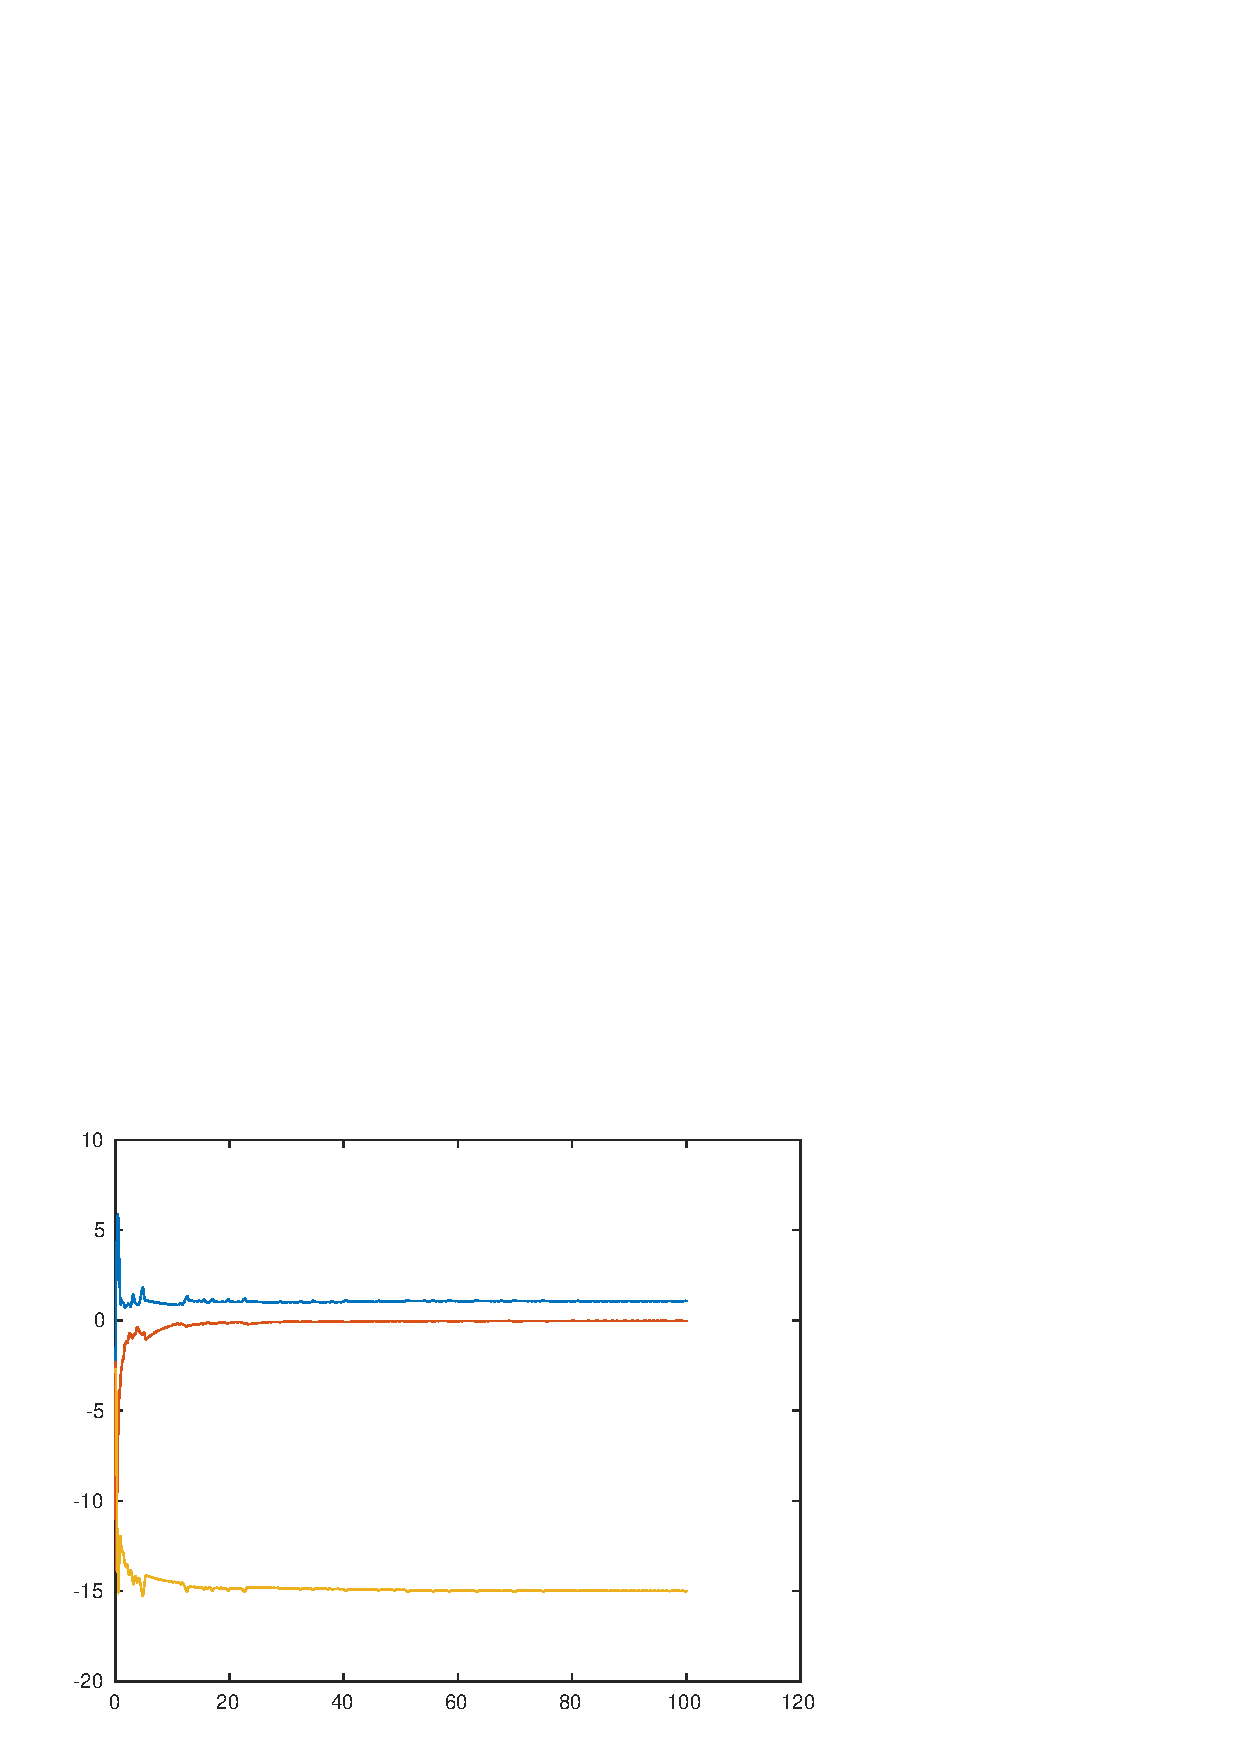
\includegraphics[scale=0.5]{./plots/goodLiapunov.pdf}
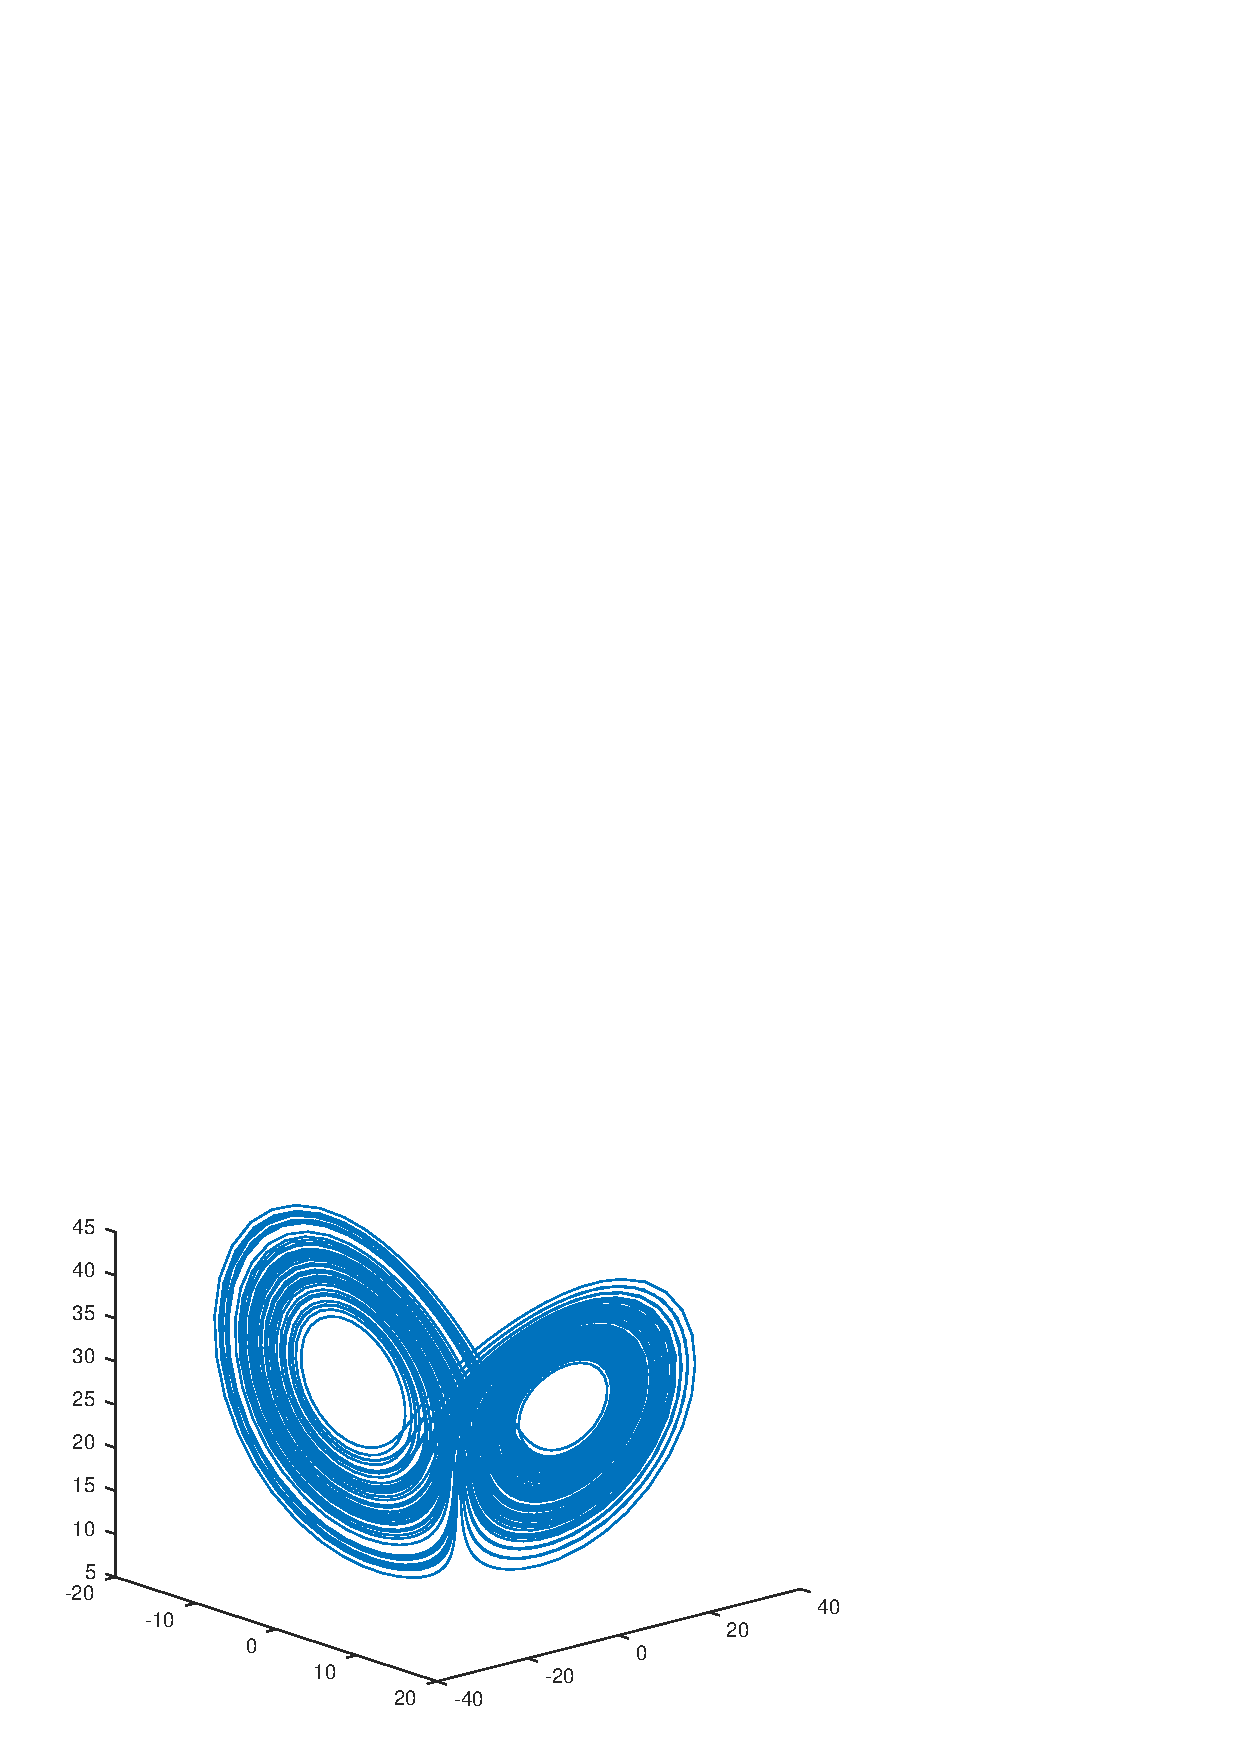
\includegraphics[scale=0.5]{./plots/goodLorenz.pdf}
\caption{\texttt{x = [0 1 20]';st = 0.01;kkmax = 10000;  lyap = 1.0749   -0.0312  -14.9990}}
\label{fig:comp2}
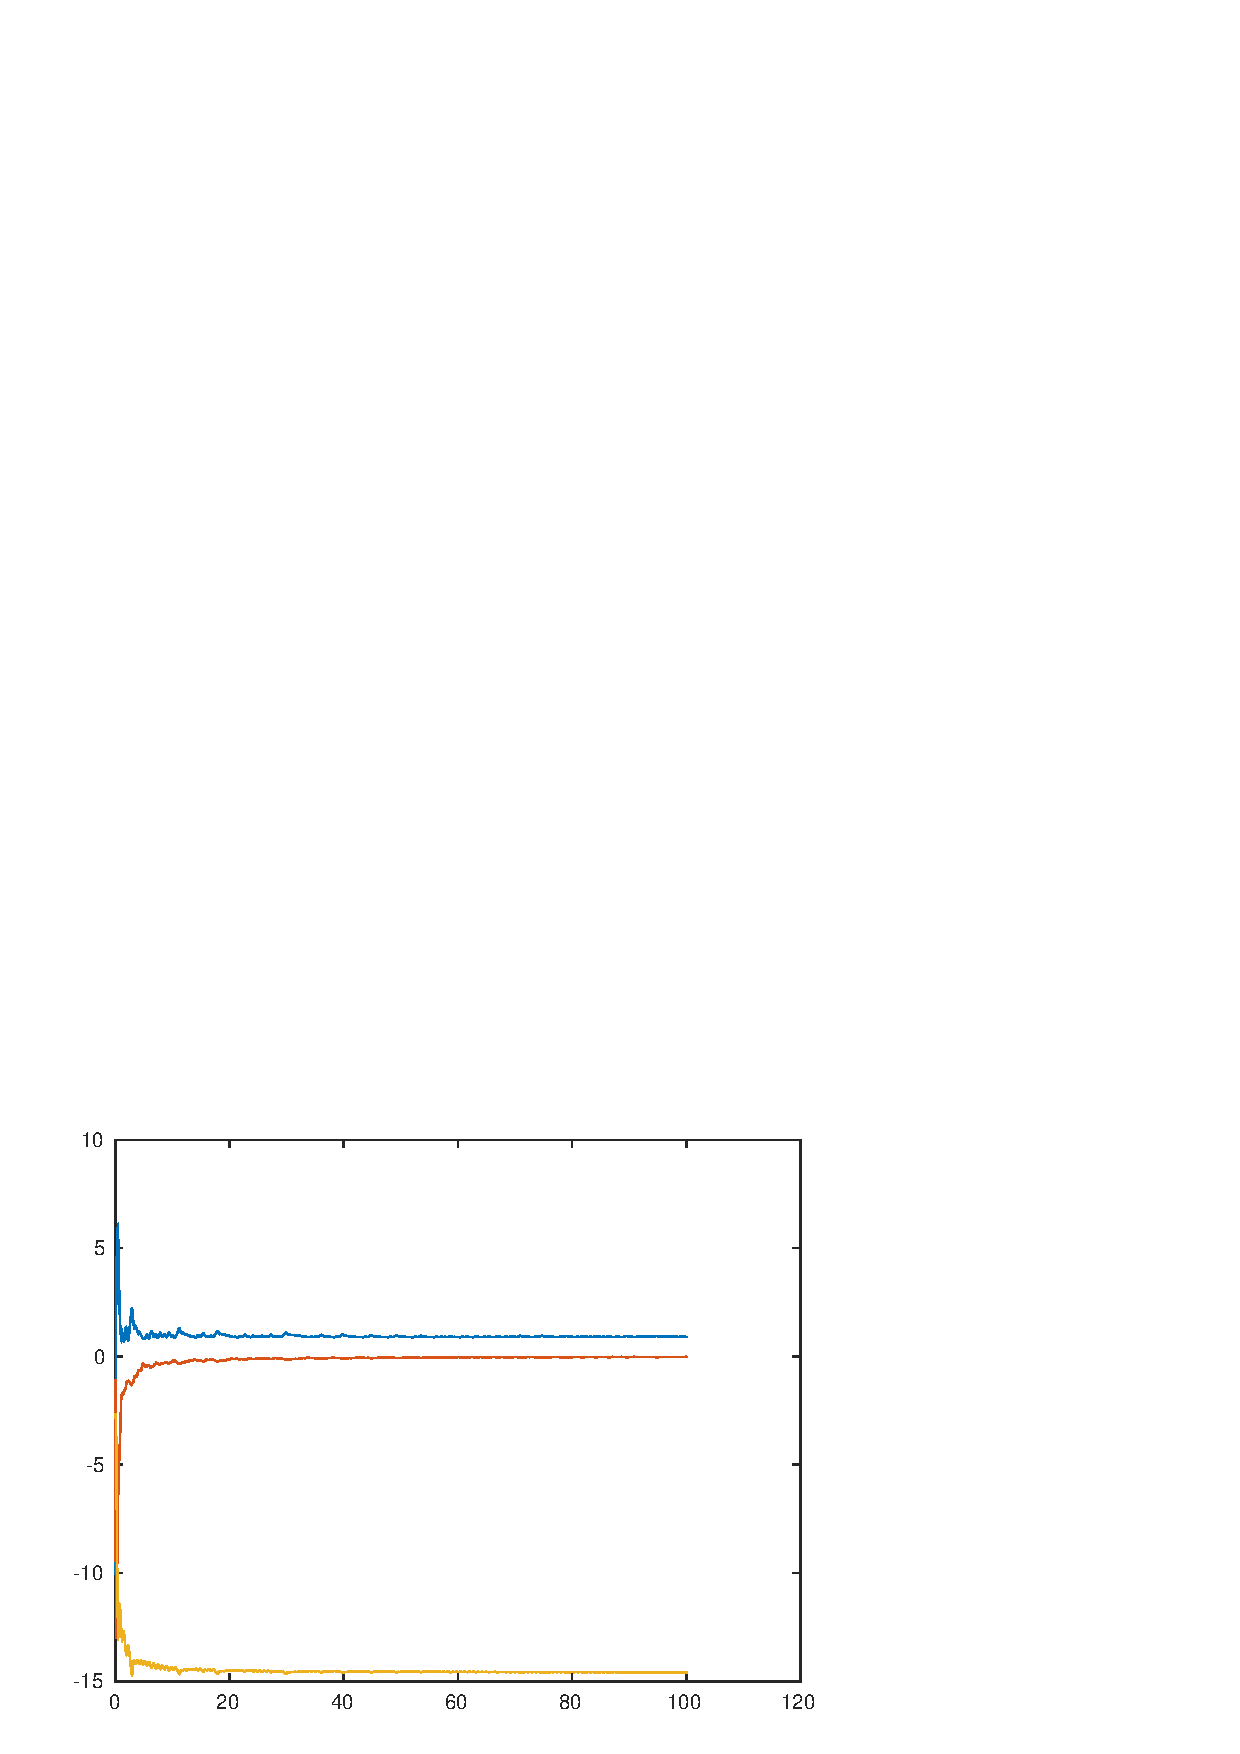
\includegraphics[scale=0.5]{./plots/bestLiapunov.pdf}
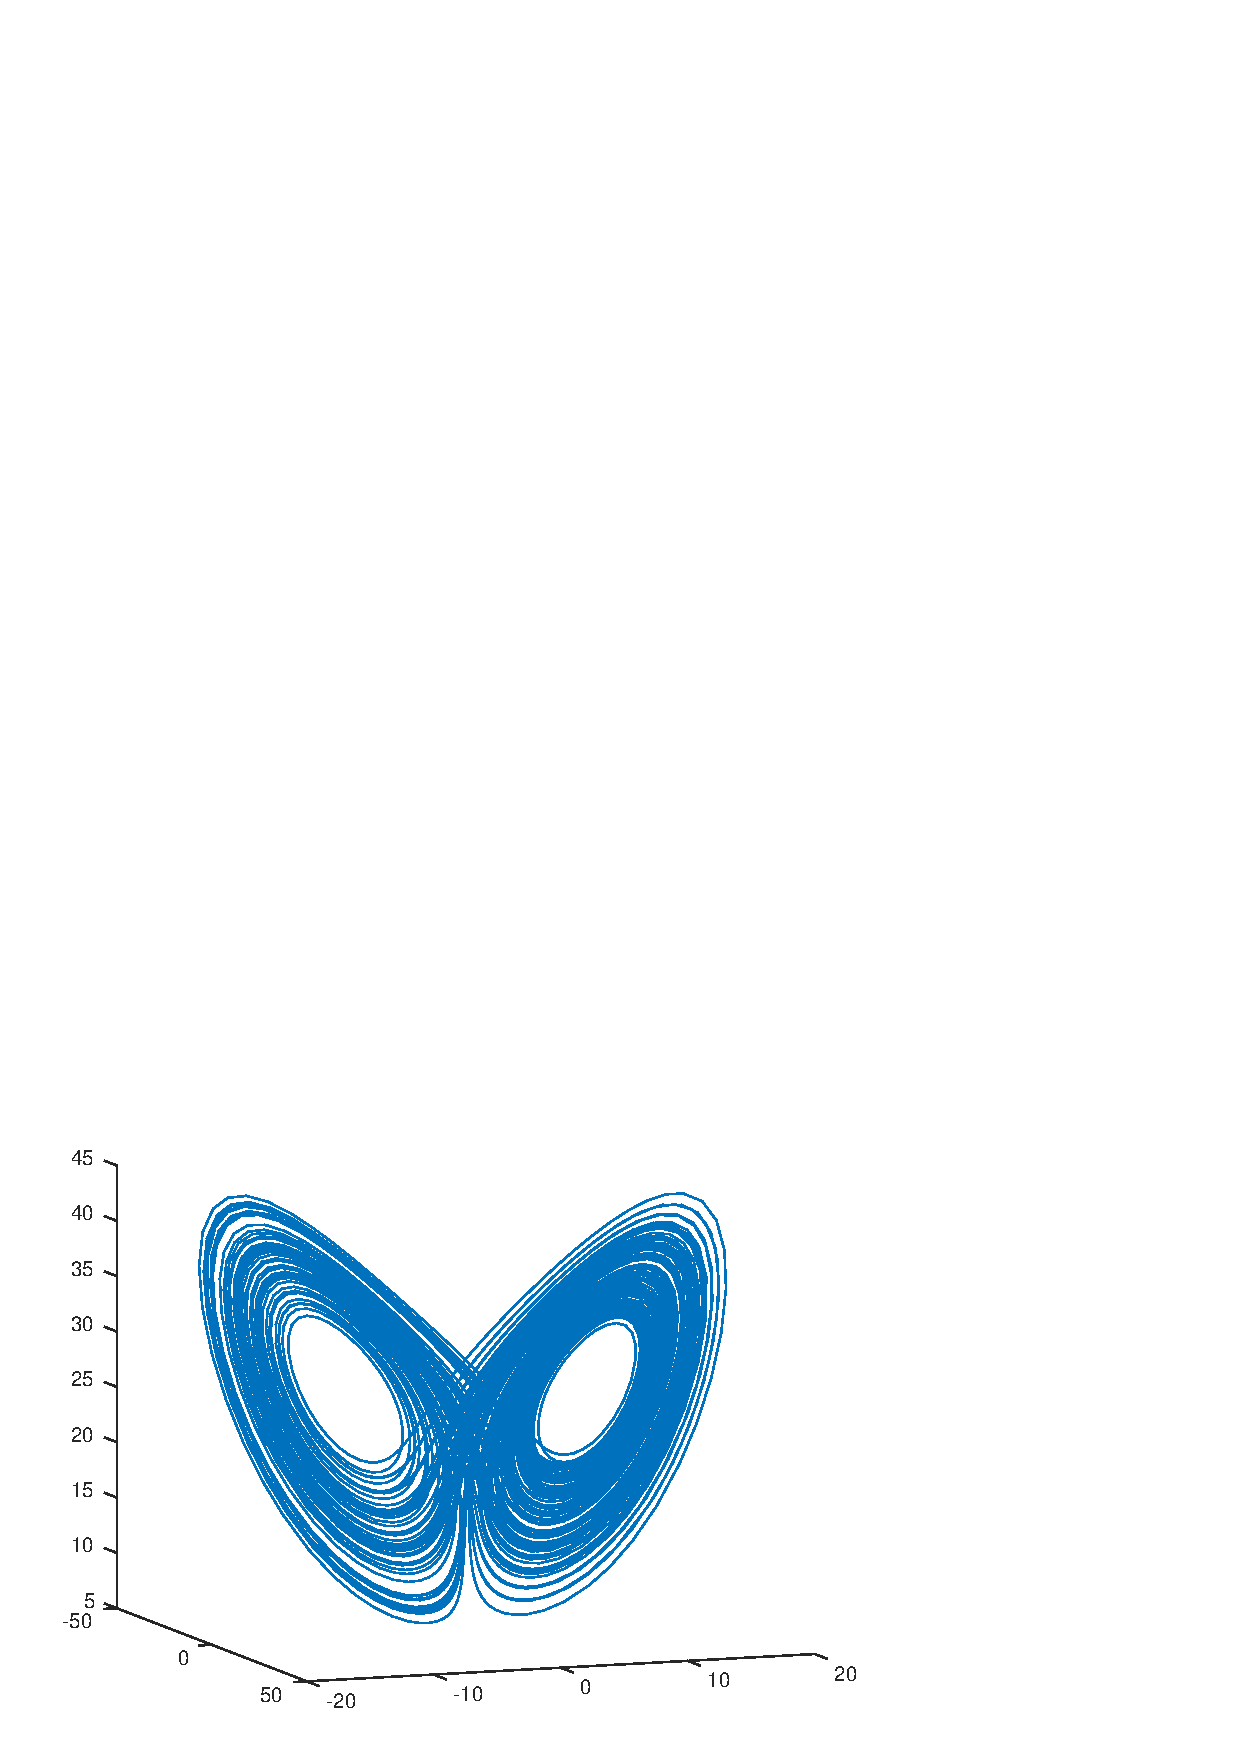
\includegraphics[scale=0.5]{./plots/bestLorenz.pdf}
\caption{\texttt{x = [0 1 20]'; st = 0.001; kkmax = 100000; lyap = 0.9035   -0.0150  -14.5896}}
\label{fig:comp3}
\end{figure}

\section{The duffing Oscillator}


\end{document}